\documentclass[12pt, twoside]{report}

\usepackage{fontspec}
\usepackage{unicode-math}
\setmainfont{Tex Gyre Pagella}
\setmathfont{TeX Gyre Pagella Math}

\usepackage[a4paper]{geometry}
\geometry{verbose,tmargin=4cm,bmargin=3cm,lmargin=4cm,rmargin=3cm}

\usepackage{fancyhdr}
\pagestyle{fancy}

\setcounter{secnumdepth}{3}
\setcounter{tocdepth}{3}

\usepackage{polyglossia}
\setmainlanguage[variant=us]{english}
\setotherlanguage[variant=brazilian]{portuguese}

\usepackage{setspace}
\onehalfspacing

\usepackage[
unicode=true,
pdfusetitle,
bookmarks=true,
bookmarksnumbered=false,
bookmarksopen=false,
breaklinks=false,
pdfborder={0 0 1},
backref=false,
colorlinks=false
]{hyperref}

\makeatletter

%%%%%%%%%%%%%%%%%%%%%%%%%%%%%%%%%%%%
%%% USER PACKAGES

\usepackage{amsmath}
\usepackage{amsthm}
\usepackage{bm}
\usepackage{mathrsfs}
\usepackage{mathtools}

\usepackage{graphicx}
\usepackage{color}

\usepackage{verbatim}
\usepackage{booktabs}
\usepackage{cancel}
\usepackage{listings}

\usepackage[svgnames]{xcolor}
\usepackage{hyperref}
\hypersetup{colorlinks=true,urlcolor=NavyBlue,linkcolor=NavyBlue,citecolor=CornflowerBlue,naturalnames=true,hypertexnames=true}

\usepackage[numbers]{natbib}

\usepackage{svg}

\usepackage{caption}
\usepackage{subcaption}

\usepackage[none]{hyphenat}
\sloppy

\usepackage{multirow}

\usepackage[withpage]{acronym}

%%%%%%%%%%%%%%%%%%%%%%%%%%%%%%%%%%%%
%%% MATH MACROS

% Upright d
\newcommand{\ud}{\mathrm{d}}

% Integration element
\usepackage{xifthen}
\newcommand{\intelm}[2] {
  \ifthenelse{\isempty{#2}}
    {\ud #1 \,}
    {\ud^{#2} {#1} \,}
}

% Derivatives
\newcommand{\der}[2]{\frac{\ud #1}{\ud #2}}
\newcommand{\del}[2]{\frac{\partial #1}{\partial #2}}
\newcommand{\nder}[3]{\frac{\ud^{#3} #1}{\ud {#2}^{#3}}}
\newcommand{\ndel}[3]{\frac{\partial^{#3} #1}{\partial {#2}^{#3}}}

% Tensors
\newcommand{\tens}[3]{#1^{#2}_{\phantom{#2} #3}}
\newcommand{\itens}[3]{#1_{#3}^{\phantom{#3} #2}}

% Covariant derivative
\newcommand{\covd}[1]{\tens{\nabla}{}{#1}}
\newcommand{\ucovd}[1]{\tens{\nabla}{#1}{}}

% Metric tensor
\newcommand{\g}{\textsl{g}}
\newcommand{\mtrtens}[2]{\tens{\g}{}{#1#2}}
\newcommand{\umtrtens}[2]{\tens{\g}{#1#2}{}}

% Kronecker delta
\newcommand{\kdelta}[2]{\tens{\delta}{#1}{#2}}

% Connection symbols
\newcommand{\chris}[3]{\tens{\Gamma}{#1}{#2 #3}}

% Index partial derivative
\newcommand{\indexdel}[1]{\tens{\partial}{}{#1}}

% References
\newcommand{\myref}[1]{Eq. (\ref{#1})}

% Definitions, theorems
\newtheorem{theorem}{Theorem}[section]
\newtheorem{definition}{Definition}[section]

% "Fat" table cells
\newcommand{\tlt}[2]{\begin{tabular}[c]{@{}c@{}}#1\\ #2\end{tabular}}

%%%%%%%%%%%%%%%%%%%%%%%%%%%%%%%%%%%%
%%% SPACING MACROS

\usepackage{slashed}

\usepackage{nextpage}
\newcommand\myclearpage{\cleartooddpage[\thispagestyle{empty}]}

\usepackage[fit]{truncate}
\fancyhf{}
\fancyhead[LE]{\truncate{.95\headwidth}{\leftmark}}
\fancyhead[RO]{\truncate{.95\headwidth}{\rightmark}}
\fancyfoot[C]{\thepage}

\makeatother

%%%%%%%%%%%%%%%%%%%%%%%%%%%%%%%%%%%%
%%% DOCUMENT START

\begin{document}

\pagenumbering{gobble}

%%%%%%%%%%%%%%%%%%%%%%%%%%%%%%%%%%%%
%%% AUTHOR'S NAME

\begin{center}
  Lucas Timotheo Sanches
  \par\end{center}

\vspace{2.5cm}

%%%%%%%%%%%%%%%%%%%%%%%%%%%%%%%%%%%%
%%% THESIS TITLE

\begin{center}
  {\huge{}Energy Extraction and Quasinormal Modes of Black Hole Binaries: An analytical and numerical study}{\huge\par}
  \par\end{center}

\begin{center}
  \vspace{2.5cm}
  \par\end{center}

%%%%%%%%%%%%%%%%%%%%%%%%%%%%%%%%%%%%
%%% THESIS DESCRIPTION

\begin{center}
  \begin{minipage}[t]{0.6\columnwidth}
    \begin{center}
      Thesis presented to the Post-Graduation program in Physics of
      Federal University of ABC as a requirement for obtaining the title
      of Doctor in Physics.
      \par\end{center}
  \end{minipage}
  \par\end{center}

%%%%%%%%%%%%%%%%%%%%%%%%%%%%%%%%%%%%
%%% ADVISORS

\begin{center}
  \vspace{2cm}
  Advisor: Prof. Dr. Maurício Richartz
  \par\end{center}

%%%%%%%%%%%%%%%%%%%%%%%%%%%%%%%%%%%%
%%% CITY

\begin{center}
  \vspace{2cm}
  Santo André - SP
  \par\end{center}

%%%%%%%%%%%%%%%%%%%%%%%%%%%%%%%%%%%%
%%% YEAR

\begin{center}
  2023
  \par\end{center}

\begin{center}
  {\large{}\thispagestyle{empty}}{\large\par}
  \par\end{center}

\begin{center}
  \pagebreak{}
  \par\end{center}

\vfill{}

%%%%%%%%%%%%%%%%%%%%%%%%%%%%%%%%%%%%
%%% LIBRARY STUFF

\begin{center}
  \fbox{\begin{minipage}[t]{0.8\columnwidth}%
      TIMOTHEO SANCHES, Lucas

      \hspace{1cm}Energy Extraction and Quasinormal Modes of Black Hole Binaries: An analytical and numerical study / Lucas Timotheo Sanches - Santo André,
      Universidade Federal do ABC, 2023.

      \vspace{0.5cm}

      \hspace{1cm}XX fls. XX cm\vspace{0.5cm}

      \hspace{1cm}\textportuguese{Orientador: Maurício Richartz}\vspace{0.5cm}

      \hspace{1cm}\textportuguese{Tese (doutorado) — Universidade}
      \textportuguese{Federal do ABC, Programa de Pós-Graduação em Física, 2023}\vspace{0.5cm}

      \hspace{1cm}
      \begin{portuguese}
        1. Palavra-chave. 2. Palavra-chave.  3. Palavra-chave.
        I. TIMOTHEO SANCHES, Lucas. II. Programa de Pós-Graduação em Física,
        2021. III. Título: subtítulo%
      \end{portuguese}
    \end{minipage}}
  \par\end{center}

\begin{center}
  {\large{}\thispagestyle{empty}}{\large\par}
  \par\end{center}

\begin{center}
  \pagebreak{}
  \par\end{center}

%%%%%%%%%%%%%%%%%%%%%%%%%%%%%%%%%%%%
%%% DEDICATION

\begin{minipage}[t]{0.9\columnwidth}%
  \begin{center}
    \textbf{\large{}\rule[0.5ex]{1\columnwidth}{1pt}}{\large\par}
    \par\end{center}
  \begin{doublespace}
    \textportuguese{DEDICATÓRIA}
  \end{doublespace}

  \rule[0.5ex]{1\columnwidth}{1pt}%
\end{minipage}
\begin{center}
  {\large{}\thispagestyle{empty}}{\large\par}
  \par\end{center}
\begin{portuguese}
  Dedico esse trabalho à memória da minha amada avó, Ignez de Sousa Timotheo, que faleceu durante a elaboração do mesmo e que durante toda a sua vida representou um exemplo inabalável de força moral e superação das piores adversidades as quais um ser humano pode ser submetido. O seu exemplo e as suas palavras estarão eternamente gravados na minha memória e no meu coração.

  Maior que o seu exemplo, era talvez somente o amor que tivera pelos filhos, e por mim, o seu único neto. Tal amor era refletido no orgulho que ela sentia em ter um neto que seria o primeiro da nossa família a tornar-se doutor. Por conta do curso natural da nossa breve existência, ela não poderá presenciar fisicamente a conclusão desse trabalho que ela vira se iniciar. Entretanto, acredito e sinto que de alguma forma, ela estará comigo, não só na minha defesa, mas indubitavelmente no meu coração e acompanhando os meus paços durante toda a minha vida.
\end{portuguese}

\begin{center}
  \myclearpage
  \par\end{center}

%%%%%%%%%%%%%%%%%%%%%%%%%%%%%%%%%%%%
%%% THANKS

\begin{minipage}[t]{0.9\columnwidth}%
  \begin{center}
    \textbf{\large{}\rule[0.5ex]{1\columnwidth}{1pt}}{\large\par}
    \par\end{center}
  \begin{doublespace}
    \textportuguese{AGRADECIMENTOS}
  \end{doublespace}

  \rule[0.5ex]{1\columnwidth}{1pt}%
\end{minipage}
\begin{center}
  {\large{}\thispagestyle{empty}}{\large\par}
  \par\end{center}

\begin{portuguese}[variant=brazilian]
  Nenhum texto pode refletir adequadamente o sentimento de gratidão que tenho pelos maiores responsáveis pelos sucessos da minha trajetória até este ponto: os meus pais, Luis e Tania. Durante toda a minha vida, os meus pais incentivaram e deram apoio ao meu instinto investigativo, ao meu interesse pela ciência e à minha paixão pelos estudos. Deram-me apoio financeiro, e principalmente, emocional e todo o seu amor nos momentos mais difíceis da minha caminhada. Sinto-me honrado de ser filho de pessoas tão maravilhosas e inigualáveis, exemplos em todos os sentidos. Amorosos. Carinhosos. Cuidadores. Pais. Espero retornar-lhes com o orgulho de ter um filho titulado doutor uma parte de todo o amor incondicional que eles tem por mim desde o meu nascimento, e demonstrar através deste trabalho uma pequena parte de toda a admiração e amor que sinto por eles.

  Agradeço, de forma igualmente carinhosa, o restante dos meus familiares, cujas características que atribuí aos meus pais de apoio, amor e a admiração que sinto por eles também se aplicam: a minha avó Marisa, o meu avô Luis e às minhas tias, Sandra e Márcia.

  Gostaria de expressar o meu sincero agradecimento a uma pessoa muito especial, que tive a sorte de conhecer durante a elaboração desse trabalho: a minha amada companheira, Thalía. Agradeço-lhe por todo o apoio e incentivo que você me deu durante o processo de elaboração da minha tese. Sem a sua ajuda, eu não teria conseguido concluir este trabalho. A sua presença foi, e ainda é, fundamental para o meu sucesso. Eu não poderia ter pedido por uma companheira mais amorosa, solidária e compreensiva nesta jornada. Este é um momento importante para mim e você contribuiu enormemente para eu chegar até aqui. Obrigado por ser minha namorada e a minha inspiração. Espero que possamos continuar a apoiar um ao outro nos nossos futuros desafios e conquistas, e que o nosso amor se fortaleça cada vez mais com os muitos anos que teremos pela frente.

  A vida, sem bons amigos, seria um erro. É por isso que agradeço profundamente àqueles que decidiram fazer parte da minha vida, minha luta e minha trajetória por livre e espontânea vontade e aqui permanecem ao meu lado mesmo dadas as dificuldades da convivência do dia a dia. São eles: Bruna, Caio, Gabriel, Karen, Rafaela, Thiago e por fim, mas não menos importante, Iara, a quem além dos anos de amizade devo agradecimentos pela troca de discussões, ajuda, opiniões, apoio e suporte, tanto em assuntos acadêmicos quanto em assuntos pessoais que foram essenciais à elaboração desse trabalho e durante a minha carreira. Que possamos continuar sempre nos apoiando em todos os aspectos das nossas vidas.

  Agradeço também a meu orientador, Maurício, por toda a orientação e apoio que você me proporcionou ao longo deste tempo. As suas orientações foram essenciais para eu poder alcançar os resultados desejados no meu trabalho. As suas críticas construtivas, sugestões e opiniões foram sempre muito valiosos para o meu crescimento pessoal e profissional. Agradeço por ter-me dedicado o seu tempo, compartilhado o seu conhecimento e ajudado a desenvolver as minhas habilidades de pesquisa. As suas orientações foram além do aspecto profissional, sempre se mostrando preocupado com o meu bem-estar e com a minha jornada acadêmica. Foi uma grande honra ter você como o meu orientador e com certeza levarei as lições aprendidas no meu futuro.
\end{portuguese}

I would also like to express my heartfelt gratitude to Dr. Erik Schnetter, my international collaborator and mentor. Your expertise in the field of numerical relativity is unparalleled, and your dedication to your research is truly inspiring. I feel incredibly fortunate to have had the opportunity to work with you and learn from you. You have not only taught me the intricacies of numerical relativity but also provided me with the necessary guidance and support to succeed in our research endeavors. Your enthusiasm for our projects has been infectious, and I have been constantly motivated by your passion for advancing scientific knowledge. I hope to continue working with you for many years to come, building on the foundation we have established together.

\begin{center}
  {\large{}\thispagestyle{empty}}{\large\par}
  \par\end{center}

\newpage

\begin{center}
  {\large{}\thispagestyle{empty}}{\large\par}
  \par\end{center}

\newpage

%%%%%%%%%%%%%%%%%%%%%%%%%%%%%%%%%%%%
%%% CAPES

\begin{center}
  This study was financed in part by the Coordenação de Aperfeiçoamento de Pessoal de Nível Superior – Brasil (CAPES) – Finance Code 001
\end{center}

\begin{center}
  {\large{}\thispagestyle{empty}}{\large\par}
  \par\end{center}

\newpage

\begin{center}
  {\large{}\thispagestyle{empty}}{\large\par}
  \par\end{center}

\newpage

%%%%%%%%%%%%%%%%%%%%%%%%%%%%%%%%%%%%
%%% ABSTRACT 1

\begin{center}
  \textbf{\large{}\rule[0.5ex]{1\columnwidth}{1pt}}{\large\par}
  \par\end{center}

\begin{center}
  \textbf{\Large{}Resumo}{\Large\par}
  \par\end{center}

\vspace{0.5cm}

\begin{portuguese}[variant=brazilian]
  Esta tese explora fenômenos clássicos em múltiplos modelos de binários de buracos negros utilizando técnicas numéricas, analíticas e semi-analíticas. Nosso estudo fornece percepções sobre a extração de energia, modos quasinormais e o espalhamento ondulatório ao redor binários de buracos negros, e demonstra como a presença de um binário altera estes fenômenos quando comparados às suas contrapartidas na presença de um único buraco negro. O estudo desenvolve técnicas inovadoras e pacotes numéricos, incluindo uma técnica para o estudo da extração de energia no contexto de espaços-tempos gerais, um código baseado no Método da Iteração Assintótica para o cálculo de frequências quasinormais de espaços-tempos de buracos negros e um novo \texttt{Thorn} para o \texttt{EinsteinTookit} para a evolução numérica de um campo escalar superimposto em uma métrica de evolução dinâmica. Estes resultados demonstram aumento da eficiência da extração de energia na presença de um objeto secundário e o cálculo bem-sucedido de novas frequências para perturbações de spin $5/2$ para o buraco negro de Schwarzschild. Descobertas preliminares do espalhamento de um campo escalar sem massa no binário do evento de colisão GW150914 demonstram percepções valiosas, mas estão sujeitas a mais testes e desenvolvimentos. Direções futuras de pesquisa incluem a incorporação da proposta de estudo do Processo de Penrose em espaços-tempos dinâmicos em simulações completamente dinâmicas, maior exploração da simulação numérica do campo escalar no topo do evento GW150914 e a inclusão de \textit{backreaction} da métrica para o aumento do realismo das simulações. As contribuições dessa tese aumentam a confiança na precisão e no potencial de métodos numéricos para a resolução de novos problemas em modelos de binários de buracos negros.
\end{portuguese}

\vspace{0.5cm}

%%%%%%%%%%%%%%%%%%%%%%%%%%%%%%%%%%%%
%%% KEYWORDS 1

\textbf{\textportuguese{Palavras-chave: Buracos Negros, Processo de Penrose, Extração de Energia, Modos Quasinormais, \texttt{EinsteinTookit}, Relatividade Numérica}}

\begin{center}
  {\large{}\thispagestyle{empty}}{\large\par}
  \par\end{center}

\newpage

\begin{center}
  {\large{}\thispagestyle{empty}}{\large\par}
  \par\end{center}

\newpage

%%%%%%%%%%%%%%%%%%%%%%%%%%%%%%%%%%%%
%%% ABSTRACT 2

\begin{center}
  \textbf{\large{}\rule[0.5ex]{1\columnwidth}{1pt}}{\large\par}
  \par\end{center}

\begin{center}
  \textbf{\Large{}Abstract}{\Large\par}
  \par\end{center}

\vspace{0.5cm}

This thesis explores classical phenomena in multiple models of black hole binaries using numerical, analytical, and semi-analytical techniques. Our study provides insights into energy extraction, quasinormal modes, and wave scattering around black hole binaries, and demonstrates how the presence of a binary alters these phenomena compared to their single black hole counterparts. The study develops innovative techniques and numerical packages, including a technique for studying energy extraction in the context of general spacetime metrics, an Asymptotic Iteration Method-based code for computing quasinormal frequencies of black hole spacetimes, and a new \texttt{EinsteinToolkit Thorn} for the numerical evolution of a scalar field superimposed on a dynamically evolving metric. The results demonstrate enhanced efficiency of energy extraction in the presence of a secondary object, and the successful computation of new quasinormal frequencies for spin $5/2$ perturbations of a Schwarzschild black hole. Preliminary findings of the scattering of a massless field over the GW150914 binary collision demonstrate valuable insights but are subject to further testing and development. Future research directions include incorporating the proposed approach for studying the Penrose process in dynamic spacetimes into fully dynamical simulations, further exploring the numerical simulation of the scalar field on top of the GW150914 binary, and considering the backreaction of the spacetime metric to enhance the realism of the simulations. The thesis's contributions enhance confidence in the accuracy and potential of numerical methods for addressing novel problems in binary black hole spacetime models.

\vspace{0.5cm}

%%%%%%%%%%%%%%%%%%%%%%%%%%%%%%%%%%%%
%%% KEYWORDS 2

\textbf{Keywords: Black Holes, Penrose Process, Energy Extraction, Quasinormal Modes, \texttt{EinsteinTookit}, Numerical Relativity}

\begin{center}
  {\large{}\thispagestyle{empty}}{\large\par}
  \par\end{center}

\newpage

\begin{center}
  {\large{}\thispagestyle{empty}}{\large\par}
  \par\end{center}

\newpage

%%%%%%%%%%%%%%%%%%%%%%%%%%%%%%%%%%%%
%%% LIST OF FIGURES

\thispagestyle{empty}
\listoffigures

\begin{center}
  {\large{}\thispagestyle{empty}}{\large\par}
  \par\end{center}

\newpage

\begin{center}
  {\large{}\thispagestyle{empty}}{\large\par}
  \par\end{center}

\newpage

%%%%%%%%%%%%%%%%%%%%%%%%%%%%%%%%%%%%
%%% LIST OF TABLES

\listoftables

\begin{center}
  {\large{}\thispagestyle{empty}}{\large\par}
  \par\end{center}

\newpage

\begin{center}
  {\large{}\thispagestyle{empty}}{\large\par}
  \par\end{center}

\newpage

%%%%%%%%%%%%%%%%%%%%%%%%%%%%%%%%%%%%
%%% LIST OF ACRONYMS

\chapter*{List of Acronyms}

\begin{acronym}
  \acro{GR}{General Relativity}
  \acro{BH}{Black Hole}
  \acro{BBH}{Binary Black Hole}
  \acro{PP}{Penrose Process}
  \acro{SKS}{Super Imposed Kerr Metric in Kerr-Schild Coordinates}
  \acro{NR}{Numerical Relativity}
  \acro{QNM}{Quasinormal Mode}
  \acro{ADM}{Arnowit, Deser and Misner}
  \acro{AMR}{Adaptive Mesh Refinement}
  \acro{CAS}{Computer Algebra System}
  \acro{AIM}{Asymptotic Iteration Method}
  \acro{API}{Application Programming Interface}
  \acro{ODE}{Ordinary Differential Equation}
  \acro{MP}{Majumdar and Papapetrou}
  \acro{CMMR}{Cabrera-Munguia, Manko and Ruiz}
\end{acronym}

\begin{center}
  {\large{}\thispagestyle{empty}}{\large\par}
  \par\end{center}

\newpage

\begin{center}
  {\large{}\thispagestyle{empty}}{\large\par}
  \par\end{center}

\newpage

%%%%%%%%%%%%%%%%%%%%%%%%%%%%%%%%%%%%
%%% TABLE OF CONTENTS

\tableofcontents{}

\begin{center}
  {\large{}\thispagestyle{empty}}{\large\par}
  \par\end{center}

\newpage

\begin{center}
  {\large{}\thispagestyle{empty}}{\large\par}
  \par\end{center}

\newpage

%%%%%%%%%%%%%%%%%%%%%%%%%%%%%%%%%%%%
%%% CHAPTERS

\pagenumbering{arabic}
\setcounter{page}{35}
\chapter{Introduction}
\label{ch:introduction}
One of the most well know predictions of the Theory of General Relativity (GR) is the existence of spacetime oscillations that propagate throughout the universe, the so called, gravitational waves. The first (indirect) evidence of the existence of such waves occurred when Hulse and Taylor observed, in 1975, the binary system PSR B1913$+$16~\cite{1975ApJ...195L..51H}. Observational data proved to be compatible with theoretical analysis for neutron star binaries that emit gravitational waves. On the other hand, direct observations, despite being attempted since the 1960's, only became a reality recently in the year 2015, with measurements from the Advanced Laser Interferometer Gravitational-wave Observatory (Advanced LIGO)~\cite{grav1,grav2} giving birth to a new era in astronomy and cosmology. These two observations have a common factor: they involve \emph{binary systems}, that is, two astronomical objects that are close enough for their mutual gravitational attraction to cause them to orbit around a common center of mass as they get closer and closer until a catastrophic collision event occurs, releasing huge amounts of energy and angular momentum in the form of gravitational radiation.

So far, no analytic description of a binary system in GR is know. This is due to the extreme complexity of Einstein's equations (a system of 10 coupled non-linear partial differential equations) whose exact solution is know only for very specific systems with a high degree of symmetry. Even if such an exact solution were to be found, it would likely be too large, complicated and and impractical to use. Given that in a collision event the nonlinear character of the equations becomes important the problem must be treated numerically, with the techniques of the field of Numerical Relativity (NR).

The main goal of our work is to investigate how classical and semi-classical effects in GR that are well know to spacetimes containing a single astrophysical object (a star or a black hole), namely the \emph{quasinormal ringdown}, \emph{the Penrose process} and \emph{Hawking radiation} extend to binary systems. To that end, we will work on two fronts: The first is a \emph{semi-analytic} approach in which we will study exact (and analytic) solutions of Einstein's equations that approximate binary black hole systems in static equilibrium. Such solutions allow us to employ numerical and semi-analytic techniques that are well know to our research group. The second is a \emph{numeric} approach in which we (with the help of international collaborators) will use numeric approximations of binary systems that are no longer in static equilibrium for our investigations.

In astrophysical contexts any excess of electric charge in a black hole tends to be quickly neutralized~\cite{gibbons1975}. For this reason, along with the existence and unicity theorems~\cite{Chrusciel2012,PhysRevLett.114.151102}, the most accepted description for an astrophysical black hole is given by the Kerr metric. Despite this fact, Einsten's equations when coupled to Maxwell's equations (a system know as the Einstein-Maxwell equations) admits solutions that represent black holes that are charged electrically and/or magnetically. The non-null electric charge allows for the existence of exact-many body solutions to the Einstein-Maxwell system. On the semi-analytic front we will make use of such charged spacetime that was obtained independently by S. D. Majumdar~\cite{MAJUMDAR1947} and A. Papapetrou~\cite{PAPAPETROU1947}, also know as the Majumdar-Papapetrou (MP) solution. This solution represents a binary system composed of two extremally charged Reissner-N\"ordstrom black holes~\cite{HARTLE1972}. Despite containing two charged static black holes, the MP solution can be considered a good approximation for a frontal collision of two non-charged black holes if their approximation velocities are much smaller than the speed of light~\cite{BINI2019}.

It's natural to ask if the MP solution can be generalized to represent systems of multiple charged Kerr-Newman black holes, which would add another degree of ``realism'' to the analytic treatment. It turns out that such generalization exists and were discovered by W. Israel, G. A. Wilson~\cite{ISRAEL1972} and A. Perj\'es~\cite{PERJES1971} and became know as the Israel-Wilson-Perj\'es (IWP) class. Unfortunately, these solutions cannot represent black holes -- they instead must always be naked Kerr-Newman singularities. In order to remain more astrophysically relevant, we will employ another class of solutions that is able to describe static Kerr binaries (and not only naked singularities) that was found very recently by Cabrera-Munguia, Manko and Ruiz (CMMR)~\cite{CABRERA2018,MANKO2019,MANKO2020}. In this solution, the Kerr binaries are kept static thanks to a massless ``strut'' that is represented by a conical singularity that keeps the black holes from colliding. Despite the ``nonphysical'' strut, such solution was used to compute the shadow of a binary black hole system and showed a good agreement with the shadow computed using a fully numerical binary system, as was shown by Cunha \emph{et. al.} in \cite{Cunha_2018}. The same group showed in \cite{Cunha_2018_2} that the massless strut does not influence the motion of photons composing the shadow.



\myclearpage
\par

\chapter{Energy Extraction From Black Hole Binaries}
\label{ch:penrose_binaries}
\section{Chapter Introduction}
\label{ch:penrose_binaries:sec:intro}
In this chapter, we will explore energy extraction from black hole binaries via the Penrose Process (PP) in black hole binaries.

The first incarnation of the PM arose as a consequence of the Kerr metric. The Kerr metric is the best know mathematical description of rotating black holes given by the theory of General Relativity~\cite{Visser:2007fj,Bambi:2011mj,Teukolsky:2014vca,berti}. Unlike static black holes, a Kerr black hole is characterized by the existence of a very peculiar region around its event horizon, known as the \emph{ergosphere} or \emph{ergoregion}. Particles that reach the ergosphere can still avoid the event horizon and, hence, are not doomed to end at the spacetime singularity. Nevertheless, any observer lying inside the ergosphere is unavoidably dragged along by the rotational motion of the black hole.

Particles inside the ergosphere may have negative energies (according to a static observer at infinity). Relying on this property, Penrose and Floyd devised a mechanism that allows one to extract energy from a rotating black hole~\cite{PENROSE1971}. The idea consists in sending a particle from infinity towards the black hole and assumes that, once inside the ergosphere, it decays into two other particles. If one of the fragments is counter-rotating with the black hole and has negative energy (which implies that the split happens inside the ergosphere), it will be captured by the black hole, meaning that the other fragment will escape to infinity. Due to the conservation of the four-momentum, the escaping fragment will have more energy and more angular momentum than the incident particle. Rotational energy and angular momentum are, thus, effectively extracted from the black hole.

Our main motivating factor for this investigation was that despite being a well-known process, the PP had not been studied in the context of black hole binaries. We have also found that many recent research endeavors attempt to establish a relation of the PP with observable astrophysical phenomena. The collisional version of the process, for instance, considers multiple particles that collide and scatter in the ergoregion, allowing  arbitrarily high center-of-mass energies. This process can potentially act as a mechanism to eliminate dark matter particles near a supermassive black hole~\cite{Schnittman:2018ccg}. The magnetic PP~\cite{Wagh1985,Tursunov:2019oiq}, on the other hand, considers charged particles and black holes surrounded by magnetic fields (originated, for instance, by plasma accretion disks around the black hole). The electromagnetic interaction allows for highly efficient energy extraction schemes, such as the one introduced in Ref.~\cite{Tursunov:2020juz} to model the emission of ultra-high energy cosmic rays from supermassive black holes. Furthermore, recent numerical simulations of plasma and jets around Kerr black holes indicate the important role that negative energy particles and the PP play on the total energy flux coming from the black hole's jets~\cite{Parfrey:2018dnc}.

A few comments on the models chosen for representing the binary systems are in order. Firstly, the nomenclature that we use to refer to a BBH is as follows:

\begin{definition}[Static/Dynamic BBH model]
    A \textbf{static} BBH model represents two black holes that \textbf{do not move} with respect to the observers that will participate in the PP. This is in contrast to a \textbf{dynamic} BBH model.
\end{definition}

\begin{definition}[Exact/Approximate BBH model]
    An \textbf{exact} BBH model is one that is an exact vacuum solution of Einstein's field equations. An \textbf{approximate} BBH model is one that is not an exact vacuum solution of said equations, and the deviation from vacuum is not considered to be an exotic type of matter but a measure of its ``non-exactness''.
\end{definition}

\begin{definition}[Analitic/Numeric BBH model]
    An \textbf{analytic} BBH model is one whose entire spacetime metric is analytically known at all points and times. In contrast, a \textbf{numeric} BBH model is obtained only at a certain coordinate time hypersurface (typically $t=0$) by solving the Arnowit-Deser-Misner (ADM) constraint equations for a vacuum configuration numerically. Note that even tough such numerical solutions contain errors, and thus do not strictly solve the vacuum field equations (giving rise to constraint violations), we do not consider these to be approximate, since it is possible (at least in theory but not in practice due to physical limitation of machines and computational resources) to obtain these solutions with arbitrarily small constraint violations given that they are convergent. For more information on solving the ADM constraint equations and obtaining initial data in Numerical Relativity, see for instance Chapter 3 of Ref~\cite{Alcubierre2012-xp}
\end{definition}

Secondly, any study that aims to model astrophysical binary systems must acknowledge the fact that there is no known exact and analytical solution of Einstein's equations describing such a system. Even if exact numerical or approximate analytical solutions are employed, the resulting spacetime metrics are non-stationary and thus limit the applicability of the standard concept of an ergosphere. Recognizing these difficulties, we have utilized BBH models that are static, exact and analytic.

Our first task was to investigate the possibility of energy extraction from the Majumdar-Papapetrou (MP) metric~\cite{MAJUMDAR1947,PAPAPETROU1947}, which is an exact solution of Einstein's equations that describes a static binary of extremally charged black holes. Despite its mathematical simplicity, the MP solution has recently been used as a surrogate model for black hole binaries in order to understand how single black hole phenomena transpose to a binary system. For instance, Ref.~\cite{ASSUMPCAO2018} has employed the MP metric to understand the connection between quasinormal modes and light rings in the context of black hole binaries. Refs.~\cite{Shipley:2016omi,Shipley:2019kfq}, on the other hand, have computed the shadows cast by an MP binary to better understand chaotic scattering in a binary black hole system. The resulting shadow shares many similarities and qualitative features with the shadows computed in Ref.~\cite{Bohn:2014xxa} using a numerically simulated binary black hole background. Ref.~\cite{BINI2019} has also applied the MP metric to analyze particle scattering around a black hole binary and asserted its effectiveness in approximating a head on collision in the limit of large separations and small approach speeds. We followed an analog approach in order to gain physical intuition and qualitative insights about energy extraction from black hole binaries by the Penrose mechanism. In particular, we extended the concept of a particle dependent \emph{generalized ergosphere}~\cite{RUFFINI1971}, which enables the extraction of electromagnetic energy from Reissner-N\"ordstrom (RN) black holes, to the MP solution and study how the energy extraction efficiency is affected by the presence of a companion black hole.

Taking into account the fact that, in astrophysical contexts, any excess of electric charge in a black hole tends to be quickly neutralized~\cite{gibbons1975}, we also considered rotating systems in our work. More specifically, in order to illustrate how the main results for the MP spacetime can be extrapolated to a binary system composed of Kerr black holes, we employ a static exact and analytic solution of Einstein's field equations, discovered independently by Cabrera-Munguia, Manko and Ruiz (hereby referred to as the CMMR metric)~\cite{cabrera_metric,manko_ruiz_metric, manko_ruiz_thermo}. The CMMR metric describes two generic Kerr black holes that do not coalesce thanks to the presence of a ``strut'' that holds them apart at a fixed distance. In particular, we sketched the ergosphere of the CMMR spacetime for a selected set of parameters and gave an example of a PP around a binary of rotating black holes.

The combined results presented in Sections \ref{ch:penrose_binaries:sec:mp_penrose} and \ref{ch:penrose_binaries:sec:cmmr_penrose} have been compiled in a paper and were published in Ref.~\cite{PhysRevD.104.124025}. As an extension to this work, we have begun the development of a framework that should allow one to observe the PP for an arbitrary spacetime and shall present these preliminary results in Sec. \ref{ch:penrose_binaries:sec:arbitrary_penrose}. We illustrate the viability of our proposition by utilizing a non-exact solution to Einstein's field equations obtained by superimposing two Kerr metric solutions in Kerr-Schild coordinates (thus called the SKS - Superimposed Kerr-Schild Kerr solution), that models an orbiting binary of rotating black holes close to merger.

\section{A brief review of the Penrose process}
\label{ch:penrose_binaries:sec:penrose_review}
In this section, we shall briefly review energy extraction of rotating and charged black holes via the Penrose Process to familiarize the reader with the underlying physical concepts, methods and techniques involved in the mechanism. This is important since these tools will be necessary later on while we present novel results.

\subsection{The Kerr spacetime}
\label{ch:penrose_binaries:sec:penrose_review:subsec:kerr}
In this section, we shall briefly review energy extraction of rotating and charged black holes via the PP to familiarize the reader with the underlying physical concepts, methods and techniques involved in the mechanism. This is important since these tools will be necessary later on while we present novel results. Our review will follow closely Ref.~\cite{carroll}. We start by reminding that the Kerr metric, in Boyer-Lindquist coordinates $(t, r, \theta, \phi)$ is given by

\begin{multline}
  \ud s^2 = -\left(1 - \frac{2 M r}{\rho^2}\right)\ud t^2 - \frac{2 M a r \sin^2\theta}{\rho^2}\left( \ud t \ud \phi + \ud \phi \ud t \right)\\
  + \frac{\rho^2}{\Delta} \ud r^2 + \rho^2 \ud\theta^2 + \frac{\sin^2\theta}{\rho^2}\left[ (r^2 + a^2)^2 - a^2\Delta\sin^2\theta \right]\ud\phi^2,
  \label{eq:kerr_penrose_review_kerr_metric}
\end{multline}
%
where
%
\begin{equation}
  \Delta(r) = r^2 - 2Mr + a^2
  \label{eq:kerr_penrose_review_kerr_delta}
\end{equation}
%
and
%
\begin{equation}
  \rho^2(r, \theta) = r^2 + a^2\cos^2\theta.
  \label{eq:kerr_penrose_review_kerr_rho}
\end{equation}

The constants $M$, $J$ and $a = J/M$ represent, respectively the black hole's mass, angular momentum and spin parameter. The metric possesses two event horizons, located at
%
\begin{equation}
  r_{H\pm} = M \pm \sqrt{M^2 - a^2}
  \label{eq:kerr_penrose_review_kerr_horizons}
\end{equation}
%
and since its components are independent of both the coordinate time $t$ and the axial angular variable $\phi$, there are global Killing vector fields $K = \partial_t$ and $R = \partial_\phi$ that generate these symmetries. Since the metric is stationary, the region where the time-like global Killing vector field changes its sign and thus static observers become prohibited does not coincide with the event horizons. In fact, one can easily see that
%
\begin{equation}
  K^\mu K_\mu = -\frac{1}{\rho^2}\left({\Delta - a^2 \sin^2\theta}\right) = -\frac{a^2 + r(r-2M)-a^2\sin^2\theta}{(r^2+a^2\cos^2\theta)^2}.
  \label{eq:kerr_penrose_review_kerr_killing_horizon_equation}
\end{equation}
%
and thus $K^\mu K_\mu = 0$ implies that the killing horizons are located at
%
\begin{equation}
  r_{K\pm} = M \pm \sqrt{M^2 - a^2\cos^2\theta}.
  \label{eq:kerr_penrose_review_kerr_killing_horizon_solution}
\end{equation}
%
which means that $r_{K+}$ is outside $r_{H+}$, coinciding with it only at the poles ($\theta=0$ or $\theta=\pi$). Notice also that using $r_{H+}$ in Eq.~\eqref{eq:kerr_penrose_review_kerr_killing_horizon_equation} yields $\Delta=0$ and thus
%
\begin{equation}
  K^\mu K_\mu = \frac{a^2}{\rho^2}\sin^2\theta \geq 0.
  \label{eq:kerr_penrose_review_kerr_killing_horizon_solution_2}
\end{equation}
%
The region that lies in-between $r_{K+}$ and $r_{H+}$ is called the \emph{ergosphere} or \emph{ergoregion}. The fact that this region is outside the event horizons and that $K^\mu K_\mu>0$ inside it is paramount to the Penrose mechanism, as we shall see further on. A mathematically accurate representation of important structures in the Kerr spacetime plotted in Kerr-Schild Cartesian coordinates for $M=1$ and $a=0.9$ can be found in Fig. \ref{fig:kerr_penrose_review_kerr_surfaces}. Starting from the exterior and moving towards the center, one first encounters the ergosphere, shaded in light green and bounded by $r_{K+}$. Following that, we have the outer event horizon, shaded in light blue and bounded by $r_{H+}$, and the inner event horizon, shaded in dark blue and bounded by $r_{H-}$. Finally, we have the inner ergosphere in dark green and bounded by $r_{K-}$ followed by the ring singularity at $r=0$. This figure is based on the interactive visualization generated by Ref.~\cite{KerrSurfaceViz}.

\begin{figure}[!ht]
  \centering
  \includesvg[width=\linewidth]{img/penrose_binaries/kerr_surfaces.svg}
  \caption{Mathematically accurate representation of a Kerr black hole of mass $M=1$ and spin $a=0.9$ plotted in Cartesian Kerr-Schild coordinates. The light green region represents the ergosphere of the black hole. This figure is based on the interactive visualization generated by Ref.~\cite{KerrSurfaceViz}.}
  \label{fig:kerr_penrose_review_kerr_surfaces}
\end{figure}

Let us now consider a particle of 4-momentum $p^\mu$ moving along a time-like geodesic in the Kerr spacetime parametrized by its proper time $\tau$. The energy of the particle along its trajectory, as measured by a static observer infinitely far away from the black hole, is given by
%
\begin{equation}
  E = -K_\mu p^\mu.
  \label{eq:kerr_penrose_review_kerr_enrgy_per_unit_mass_full}
\end{equation}
%
Outside the ergosphere, $K^\mu$ is time-like and $K_\mu p^\mu<0$. Since we would like the energy to be positive infinitely far away from the BH, we must introduce a leading minus sign in Eq.~\eqref{eq:kerr_penrose_review_kerr_enrgy_per_unit_mass_full}. On the other hand, inside the ergosphere $K^\mu$ is space-like and $K_\mu p^\mu >0$ which implies that in this region $E < 0$. It is important to remark that, despite the energy being negative relatively to a static observer at infinity, it still remains positive according to a local observer. Furthermore, it can be shown that these negative energy orbits must be confined within the ergosphere and must always cross the outer horizon~\cite{Grib:2013hxa,Contopoulos1984}, so there is no risk of such negative energy particles ``leaking out'' to infinity.

Let us now consider a scenario where a particle marked as $(0)$ moves through the Kerr spacetime from infinity with 4-momentum $p^{(0)\mu}$. Suppose this particle disintegrates within the ergosphere at a specific point called the break-up point $b$. This break-up results in the formation of two other particles, one marked as $(1)$, with 4-momentum $p^{(1)\mu}$, that gets absorbed by the black hole, and the other labeled as $(2)$, with 4-momentum $p^{(2)\mu}$, which escapes the gravitational pull of the system and returns to infinity. The law of conservation of 4-momentum applied at point $b$ implies that
%
\begin{equation}
  p^{(0)\mu} = p^{(1)\mu} + p^{(2)\mu}.
  \label{eq:kerr_penrose_review_kerr_4_momentum_conservation}
\end{equation}
%
Contracting Eq.~\eqref{eq:kerr_penrose_review_kerr_4_momentum_conservation} with $K^\mu$ we get
\begin{equation}
  E^{(0)} = E^{(1)} + E^{(2)}.
  \label{eq:kerr_penrose_review_kerr_energy_conservation}
\end{equation}
%
If we engineer the trajectory of particle $(1)$ such that $E^{(1)} < 0$, we get
\begin{equation}
  E^{(2)} = E^{(0)} + E^{(1)} > E^{(0)},
  \label{eq:kerr_penrose_review_kerr_energy_increase}
\end{equation}
%
which means that the energy of the returning particle is greater than the energy of the original particle. This mechanism is precisely the one proposed by Penrose and Floyd, and is therefore known as the \emph{Penrose Process} (PP) or \emph{Penrose Mechanism}. This break-up process is represented in Fig.~\ref{fig:kerr_penrose_review_kerr_breakup}.

\begin{figure}[!ht]
  \centering
  \includesvg[width=\linewidth]{img/penrose_binaries/kerr_breakup.svg}
  \caption{Schematic representation of a PP. A particle of energy $E^{(0)}$ (red) comes in from infinity and decays at point $b$ inside the ergosphere in a negative energy $E^{(1)}$ trajectory (black) and a positive energy $E^{(2)}>E^{(0)}$ trajectory (blue) that returns to infinity. The black hole's rotational axis is pointing outside the page, towards the reader.}
  \label{fig:kerr_penrose_review_kerr_breakup}
\end{figure}

Where does the excess energy of particle $(2)$ comes from? To answer that, let us analyze particle $(1)$ as it crosses the outer horizon. In the Kerr metric, the event horizons are Killing horizons of the Killing vector formed by a linear combination of the two spacetime symmetries, namely
%
\begin{equation}
  \chi^\mu = K^\mu + \Omega R^\mu
  \label{eq:kerr_penrose_review_kerr_killing_horizon}
\end{equation}
%
where $\Omega$ is the horizon's angular velocity. Considering that particle $(1)$ crosses the event horizon while remaining time-like and $\chi^\mu$ is null at the outer horizon, we must have that
%
\begin{equation}
  p^{(1)\mu}\chi_\mu = -E^{(1)} + \Omega L^{(1)} < 0
  \label{eq:kerr_penrose_review_kerr_energy_momentum_inequality}
\end{equation}
%
where $L^{(1)}$ represents the particle's angular momentum. In order to satisfy Eq.~\eqref{eq:kerr_penrose_review_kerr_energy_momentum_inequality} given that $E^{(1)} < 0$ and $\Omega > 0$ we must have that
%
\begin{equation}
  L^{(1)} < \frac{E^{(1)}}{\Omega},
  \label{eq:kerr_penrose_review_kerr_energy_momentum_inequality_L}
\end{equation}
%
which implies that $L^{(1)} < 0$ and thus the negative energy particle must be rotating in the opposite direction of the black hole. This means that when the negative energy particle gets absorbed, the BH loses a small amount of its own angular momentum, transferring it to the particle that is to be ejected back to infinity.

At this stage, one may contemplate whether it is feasible to extract all the matter from the black hole using repeated Penrose Processes (PPs). Christodoulou, in Ref.~\cite{CHRISTODOULOU1970}, has identified a restriction on energy extraction. This limitation is expressed as an irreducible mass, which represents the minimum mass that a black hole can have, and beyond which no further energy can be extracted. To see that, let us consider that when particle $(1)$ interacts with the BH, energy is conserved and thus the loss in mass and angular momentum of the black hole corresponds respectively to $E^{(1)}$ and $L^{(1)}$, that is,
%
\begin{align}
  \ud M & = E^{(1)} \label{eq:kerr_penrose_review_kerr_mass_change}, \\
  \ud J & = L^{(1)} \label{eq:kerr_penrose_review_kerr_L_change}.
\end{align}
%
By virtue of Eq.~\eqref{eq:kerr_penrose_review_kerr_energy_momentum_inequality_L}, we get that
%
\begin{equation}
  \ud J < \frac{\ud M}{\Omega}.
  \label{eq:kerr_penrose_review_kerr_energy_momentum_inequality_L_diff}
\end{equation}
%
The maximum energy extraction occurs when Eq.~\eqref{eq:kerr_penrose_review_kerr_energy_momentum_inequality_L_diff} is saturated and $\ud J = \frac{\ud M}{\Omega}$. Given that
%
\begin{equation}
  \Omega = \frac{a}{r_{H+}^2 + a^2}
  \label{eq:kerr_penrose_review_kerr_angular_momentum_def}
\end{equation}
%
we can solve
%
\begin{equation}
  \frac{\ud M}{\ud J} = \frac{a}{r_{H+}^2 + a^2}
  \label{eq:kerr_penrose_review_kerr_mass_ODE}
\end{equation}
%
for $M(J)$ with $M(0) = M_0$ to find
%
\begin{equation}
  M_0^2 = \frac{1}{2}\left( M^2 + \sqrt{M^4 - J^2} \right),
  \label{eq:kerr_penrose_review_kerr_irreducible_mass}
\end{equation}
%
which is known as the \emph{irreducible mass}. To see why that is the case, one can take the differential off Eq.~\eqref{eq:kerr_penrose_review_kerr_irreducible_mass} to find
%
\begin{equation}
  \ud M_0 = \frac{a}{4 M_0 \sqrt{M^2 - a^2}}\left( \Omega^{-1} \ud M - \ud J \right).
  \label{eq:kerr_penrose_review_kerr_irreducible_mass_diff}
\end{equation}
%
Thanks to Eq.~\eqref{eq:kerr_penrose_review_kerr_energy_momentum_inequality_L_diff}, we can infer from Eq.~\eqref{eq:kerr_penrose_review_kerr_irreducible_mass_diff} that $\ud M_0 > 0$ always, thus $M_0$ cannot be reduced (hence its name) and gives the lower energy bound that the black hole can achieve. The formula for the maximum energy that can be extracted is thus
%
\begin{equation}
  M - M_0 = M - \frac{1}{\sqrt{2}}\left( M^2 + \sqrt{M^4 - J^2} \right)^{1/2}.
  \label{eq:kerr_penrose_review_kerr_max_energy_formula}
\end{equation}
%
By considering an extreme BH (with $a=1$), Eq.~\eqref{eq:kerr_penrose_review_kerr_max_energy_formula} states that approximately $29\%$ of the BH's energy can be extracted via the PP. One can get to the same conclusion by starting of with Hawking's area theorem, which states that the event horizon area cannot decrease (See Ref.~\cite{carroll} page 270).

\subsection{The Reissner-N\"ordstrom spacetime}
\label{ch:penrose_binaries:sec:penrose_review:subsec:kerr}
Review RN

\section{Majumdar-Papapetrou Spacetime}
\label{ch:penrose_binaries:sec:mp_penrose}
The Majumdar-Papapetrou (\ac{MP}) spacetime is a static electrovacuum solution of Einstein's equations that represents a set of extremal black holes whose mutual gravitational attraction is cancelled by their mutual electromagnetic repulsion~\cite{MAJUMDAR1947,PAPAPETROU1947,HARTLE1972}.
For two black holes of masses $M_1$ and $M_2$ and electric charges $Q_1=M_1$ and $Q_2=M_2$, in equilibrium and separated by a distance $2a$ along the $z$-axis, the \ac{MP} line element, in Weyl's cylindrical coordinates $(t,\rho,\phi,z)$, is given by~\cite{SMERAK2016}
\begin{equation}
  d s^2 = - \frac{d t^2}{U(\rho,z)^{2}} + U(\rho,z)^2\left[d\rho^2 + \rho^2 d\phi^2 + d z^2\right],
  \label{eq:majumdar_papapetrou_line_element}
\end{equation}
%
where
\begin{equation}
  U(\rho,z) = 1 + \frac{M_1}{\sqrt{\rho^2 + (z+a)^2}} + \frac{M_2}{\sqrt{\rho^2 + (z-a)^2}}.
  \label{eq:mp_metric_potential_cylindric}
\end{equation}
The electromagnetic potential $A_\mu$ associated with the \ac{MP} solution is
\begin{equation}
  A_\mu = \left(1 - \frac{1}{U}\right) \delta_{\mu t},
  \label{eq:electromagnetic_potential_mp}
\end{equation}
where $\delta_{\mu \nu}$ is the Kronecker delta. We note that Weyl's coordinates describe only the exterior of the black holes. The event horizons and the black holes themselves are collapsed into the points $\rho=0, \, z=\pm a$. We denote the total mass of the binary system by $M_T=M_1+M_2$ and its mass ratio by $M_R=M_2/M_1$. Without loss of generality, we assume that $0 \le M_R \le 1$.

Being described by a static metric, the \ac{MP} spacetime does not possess an ergosphere in the sense described in Sec.~\ref{ch:penrose_binaries:sec:penrose_review}. Consequently, the energy associated with geodesic motion in the \ac{MP} spacetime is always positive, meaning that energy extraction by free particles is impossible. Charged particles, however, interact with charged black holes through Lorentz forces and, hence, do not follow geodesics.
If the electromagnetic interaction is attractive, negative energy trajectories and energy extraction are, in principle, possible. For a single charged black hole described by the RN metric, the fact that the \ac{PP} is viable was shown in Ref.~\cite{DENARDO1973}. Building on the notion of a generalized ergosphere~\cite{RUFFINI1971,DENARDO1973}, we shall study the motion of charged particles around the \ac{MP} spacetime to investigate the possibility of negative energy motion and energy extraction.

\subsection{Motion of charged particles in \ac{MP}}
\label{sec:motion}

The motion of a massive charged test particle (with charge-to-mass ratio $\mu$) in a spacetime with metric $g_{\mu \nu}$, subject to the electromagnetic potential $A_{\mu}$, is determined by the Lagrangian
\begin{equation}
  \mathcal{L} = \frac{1}{2}g_{\mu \nu}\dot{x}^\mu \dot{x}^\nu - \mu A_{\alpha}\dot{x}^\alpha,
  \label{eq:lagrangian_for_charged_particle}
\end{equation}
where $x^{\mu} = x^{\mu}(\lambda)$ denotes the position of the particle at proper time $\lambda$ and the dots represent derivatives with respect to $\lambda$. Adopting Weyl's cylindrical coordinates, and taking into account the explicit form of the \ac{MP} metric, the Lagrangian above can be recast as~\cite{RYZNER2015}
%
\begin{equation}
  \mathcal{L} = \frac{1}{2}\left[-\frac{\dot{t}^2}{U^2} + U^2\left( \dot{\rho}^2 + \rho^2\dot{\phi}^2 + \dot{z}^2 \right) \right] - \mu\left(1-\frac{1}{U}\right)\dot{t}.
  \label{eq:explicit_lagrangian_for_charged_particle}
\end{equation}
%
Since the Lagrangian does not depend explicitly on $t$ and $\phi$, two constants of motion (as measured by freely-falling observers at infinity) can be readily identified. The constant associated with the time symmetry is the energy divided by the mass $m$ of the particle:
%
\begin{equation}
  E = -\del{\mathcal{L}}{\dot{t}} = \frac{\dot{t}}{U^2} + \mu\left(1-\frac{1}{U}\right).
  \label{eq:conserved_energy}
\end{equation}
%
The constant associated with the angular symmetry is the angular momentum per unit mass (with respect to the $z$ axis):
%
\begin{equation}
  L = \del{\mathcal{L}}{\dot{\phi}} = U^2 \rho^2 \dot{\phi}.
  \label{eq:conserved_momentum}
\end{equation}

Given that the particle is following a time-like trajectory, its 4-velocity is subjected to the normalization condition
%
\begin{equation}
  \mtrtens{\mu}{\nu} \dot{x}^\mu \dot{x}^\nu = -\frac{\dot{t}^2}{U^2} + U^2\left( \dot{\rho}^2 + \rho^2\dot{\phi}^2 + \dot{z}^2 \right) = -1.
  \label{eq:4_velocity_normalization_condition_mp}
\end{equation}
%
Solving Eq.~\eqref{eq:conserved_energy} for $\dot{t}$ and Eq.~\eqref{eq:conserved_momentum} for $\dot{\phi}$ and substituting the results back into Eq.~\eqref{eq:4_velocity_normalization_condition_mp}, we obtain a quadratic equation for $E$, which in turn can be solved to yield
%
\begin{equation}
  E = \mu\left(1-\frac{1}{U}\right) + \sqrt{\frac{L^2}{\rho^2U^4} + \frac{1}{U^2} + \dot{\rho}^2 + \dot{z}^2},
  \label{eq:alternative_expression_for_energy}
\end{equation}
%
where the negative root has been ignored due to the fact that $E$ must be positive for particles at infinity when $\mu = 0$ (see Ref.~\cite{RUFFINI1971} for a detailed discussion about positive and negative root states for $E$). We note that Eq.~\eqref{eq:alternative_expression_for_energy} reduces to the expression found in Ref.~\cite{DENARDO1973} for a RN black hole if the mass of one of the black holes is taken to be zero and an appropriate coordinate system, centered around the other black hole, is adopted. For convenience and later use, we rewrite Eq.~\eqref{eq:alternative_expression_for_energy} as
\begin{equation} \label{eq:effective1}
  \dot{\rho}^2 + \dot{z}^2 = E_{\mathrm {eff}}^2(\rho,z) - V_{\mathrm {eff}}(\rho,z),
\end{equation}
where
\begin{equation} \label{eq:effective2}
  E_{\mathrm {eff}}(\rho,z) = E - \mu\left(1-\frac{1}{U}\right),
\end{equation}
and
\begin{equation} \label{eq:effective3}
  V_{\mathrm {eff}}(\rho,z) =\frac{L^2}{\rho^2U^4} + \frac{1}{U^2}.
\end{equation}
Note that the quantities defined above are subject to the following constraints:
\begin{equation} \label{eq:effective_constraints}
  E_{\mathrm {eff}}(\rho,z) \ge 0, \qquad E_{\mathrm {eff}}^2(\rho,z) \ge V_{\mathrm {eff}}(\rho,z).
\end{equation}

The equations of motion are obtained directly from the Euler-Lagrange equations. After using Eqs.~\eqref{eq:conserved_energy} and \eqref{eq:conserved_momentum} to eliminate $\dot{t}$ and $\dot{\phi}$, one is left with
%
\begin{align}
  \ddot{\rho} & -\frac{L^2(U +\rho \partial_{\rho}U)}{\rho^3 U^5} + \frac{2\dot{\rho}\dot{z}\partial_{z}U - (E^2 + \dot{z}^2 - \dot{\rho}^2)\partial_{\rho}U}{U} \nonumber \\ & \hspace{1.5cm} - \frac{\mu}{U}\left(\mu-2 E+\frac{E-\mu}{U}\right)\partial_{\rho}U = 0,
  \label{eq:ode_for_rho_motion}
\end{align}
%
and
\begin{align}
  \ddot{z} - \frac{L^2\partial_{z}U}{\rho^2 U^5} & + \frac{2\dot{\rho}\dot{z}\partial_{\rho}U - (E^2 - \dot{z}^2 + \dot{\rho}^2)\partial_{z}U}{U} \nonumber \\ &-  \frac{\mu}{U}\left(\mu-2 E+\frac{ E-\mu}{U}\right)\partial_{z}U = 0,
  \label{eq:ode_for_z_motion}
\end{align}
which reduce to the equations of motion found in Ref.~\cite{ASSUMPCAO2018} for neutral particles when $\mu=0$. Together with Eqs.~\eqref{eq:conserved_energy} and \eqref{eq:conserved_momentum}, the two equations above fully determine the trajectory of a massive charged particle in the \ac{MP} spacetime once appropriate initial conditions have been specified. In fact, we first specify the energy $E$, the angular momentum $L$, and the initial values for $\rho$, $z$, and $\dot z$. The initial value for $\dot{\rho}$ is determined from Eq.~\eqref{eq:alternative_expression_for_energy}. Using this information, we can solve the system of equations \eqref{eq:ode_for_rho_motion}-\eqref{eq:ode_for_z_motion} to obtain $\rho(\lambda)$ and $z(\lambda)$. The final step is the integration of Eqs.~\eqref{eq:conserved_energy} and \eqref{eq:conserved_momentum}, subject to the initial data for $t$ and $\phi$, to find $t(\lambda)$ and $\phi(\lambda)$.

\subsection{Generalized Ergosphere} \label{Sec:gen_ergo}

We want to know if charged particles can have negative energies in the \ac{MP} spacetime. From Eq.~\eqref{eq:alternative_expression_for_energy} it is evident that, for fixed $\mu$, the energy is completely determined by the angular momentum $L$, and the values of $\rho$, $z$, $\dot{\rho}$ and $\dot{z}$  at any given instant of time. At a fixed position, the minimum possible energy is associated with particles at rest. Letting $\dot{\rho}=\dot{z}=0$ and $L=0$ (i.e.~$\dot{\phi}=0$), we conclude that the minimum energy (per unit mass) allowed for a particle sitting at $(t,\rho,\phi,z)$ is
\begin{equation} \label{eq:minimum_energy}
  E_{\mathrm{min}} = \mu\left(1-\frac{1}{U}\right) + \frac{1}{U}.
\end{equation}

This minimum energy will be negative if the following two conditions are satisfied: Since $U \ge 1$, $\mu$ must be negative, meaning that the charge of the particle must be opposite to the charge of the black holes. Additionally, the resting particle must be inside the spatial region determined by
\begin{equation} \label{eq:rescaled_negative_energy_condition}
  \frac{1}{\sqrt{\overline{\rho}^2 + (\overline{z}+1)^2}} + \frac{M_R}{\sqrt{\overline{\rho}^2 + (\overline{z}-1)^2}} > - \frac{1+M_R}{\overline{\mu}},
\end{equation}
where $\overline{\rho} = \rho/a$, $\overline{z} = z/a$ and $\overline \mu =  \mu M_T/a$ are dimensionless quantities. The parameter $\overline \mu$ can be understood as a measure of the potential energy (per unit particle mass) associated with the electromagnetic interaction between the particle and the binary.
The inequality above determines the generalized ergosphere of the \ac{MP} spacetime: particles with opposite charge in relation to the black hole and located inside the region determined by Eq.~\eqref{eq:rescaled_negative_energy_condition} will have negative energies if their velocities are sufficiently small. Particles outside, on the other hand, will have positive energies regardless of their velocities.

\begin{figure}[!ht]
  \centering
  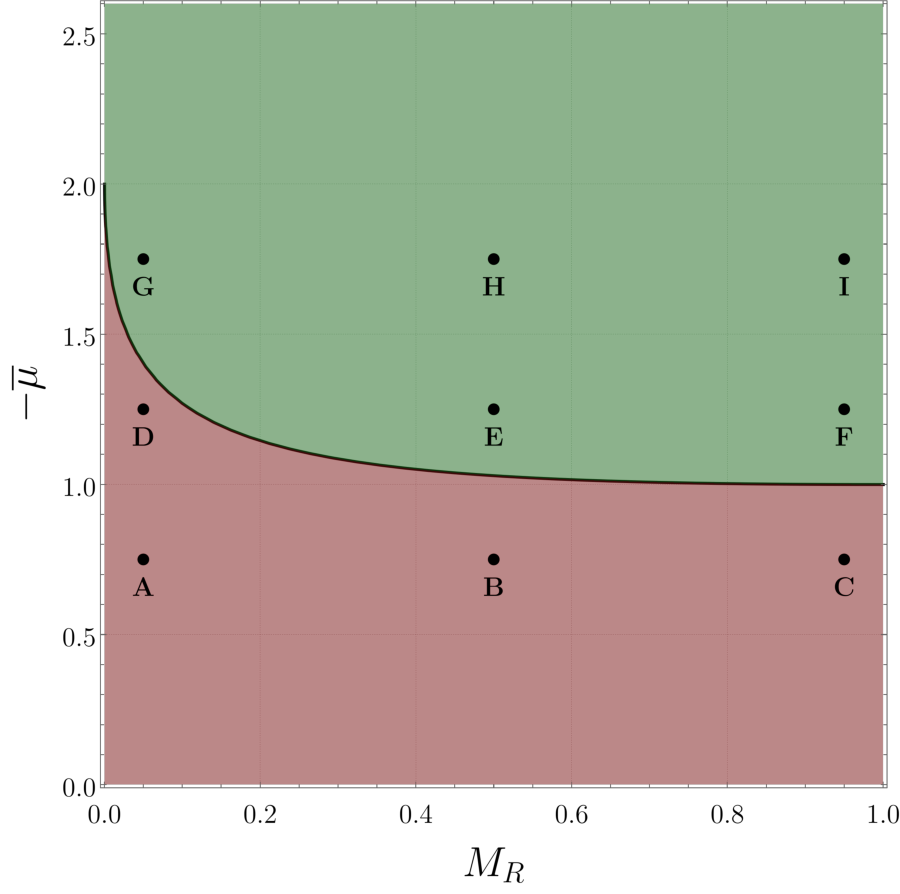
\includegraphics[width=\linewidth]{img/penrose_binaries/fig1.pdf}
  \caption{The parameter space $M_R$-$\overline \mu$. The generalized ergosphere exists if and only if $\overline \mu < 0$. It consists of a single connected region for any point inside the red section. For points in the green section, on the other hand, the ergosphere is the disjoint union of two connected regions. The black curve marks the boundary between connected and disconnected ergospheres. The ergospheres associated with the black labeled dots are plotted in Fig.~\ref{fig:ergos}.}
  \label{fig:regions}
\end{figure}

Note that the notion of a generalized ergosphere depends not only on the geometry of the spacetime, but also on properties of the particle (through the charge-to-mass ratio $\mu$), as in Refs.~\cite{RUFFINI1971,DENARDO1973}. In particular, the shape of the ergosphere depends only on the parameters $M_R$ and $\overline \mu$. In order to understand this dependence, we plot the generalized ergosphere for nine $M_R$-$\overline \mu$ pairs. Each pair corresponds to a point in the parameter space of Fig.~\ref{fig:regions} and is labeled by a letter (\textbf{A}-\textbf{I}). The $\phi=0$ section of the associated ergospheres are shown in Fig.~\ref{fig:ergos}. Due to the axial symmetry of the problem, the ergospheres are the solids of revolution obtained by the rotation of the regions shown in Fig.~\ref{fig:ergos} with respect to the $\overline z$-axis. Note that the generalized ergosphere can be either a single connected region (for parameters inside the red section of Fig.~\ref{fig:regions}) or the disjoint union of two connected regions\footnote{In such a case we shall refer to each connected region as a single ergosphere.} (for parameters in the green section of Fig.~\ref{fig:regions}). The boundary separating connected and disconnected ergospheres, represented by the black line in Fig.~\ref{fig:regions}, corresponds to the saturation of Eq~\eqref{eq:rescaled_negative_energy_condition}.

\begin{figure}[!ht]
  \centering
  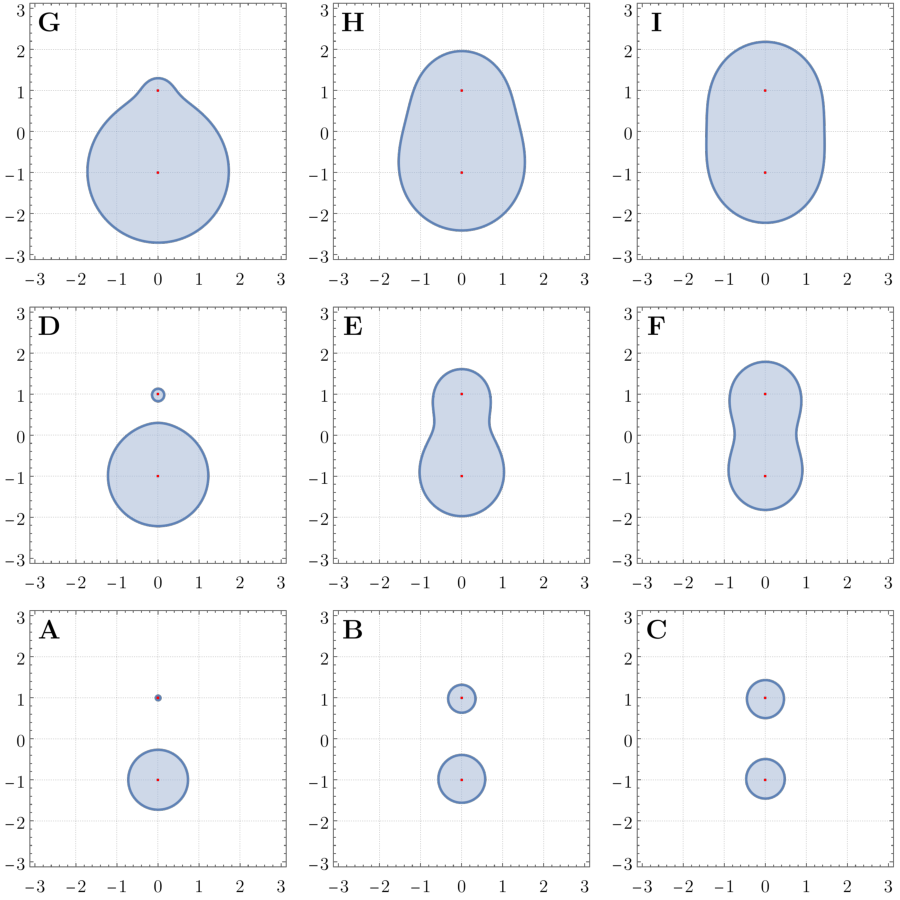
\includegraphics[width=\linewidth]{img/penrose_binaries/fig2.pdf}
  \caption{The $\phi=0$ section of the ergosphere for different points (labeled \textbf{A}-\textbf{I}) in the parameter space of Fig.~\ref{fig:regions}. In each plot the horizontal and vertical axes are $\overline \rho$ and $\overline z$, respectively. The red dots indicate the location of the black holes.}
  \label{fig:ergos}
\end{figure}

The ergosphere becomes more evenly distributed around the black holes when the mass ratio $M_R$ approaches one. This is seen in Fig.~\ref{fig:regions} by following the points \textbf{A} $\rightarrow$ \textbf{B} $\rightarrow$ \textbf{C}, or \textbf{D} $\rightarrow$ \textbf{E} $\rightarrow$ \textbf{F}, or \textbf{G} $\rightarrow$ \textbf{H} $\rightarrow$ \textbf{I}. Furthermore, if $-2 < \overline \mu < -1$, we see that an increase in the mass ratio may produce a single ergosphere from two disjoint ones, as in \textbf{D} $\rightarrow$ \textbf{E}. Similarly, for any mass ratio, an increase in the absolute value of $\overline \mu$ can also induce the merger of the ergospheres, as in \textbf{D} $\rightarrow$ \textbf{G}, \textbf{B} $\rightarrow$ \textbf{E} and \textbf{C} $\rightarrow$ \textbf{F}. In fact, no matter what the mass ratio is, if $-\overline \mu$ is sufficiently small, each black hole will be surrounded by its own ergosphere. In contrast, if $-\overline \mu$ is sufficiently large, there will be a single ergosphere surrounding the binary black hole. Finally, we remark that, according to Eq.~\eqref{eq:rescaled_negative_energy_condition}, the effects of the charge of the particle, of the total mass of the binary and of the separation parameter are all combined in $\overline \mu$. Therefore, as far as the visualization of the ergosphere is concerned, the effect of increasing $|\mu|$ is exactly the same as increasing $M_T$ or decreasing $a$.

\begin{figure}[!ht]
  \centering
  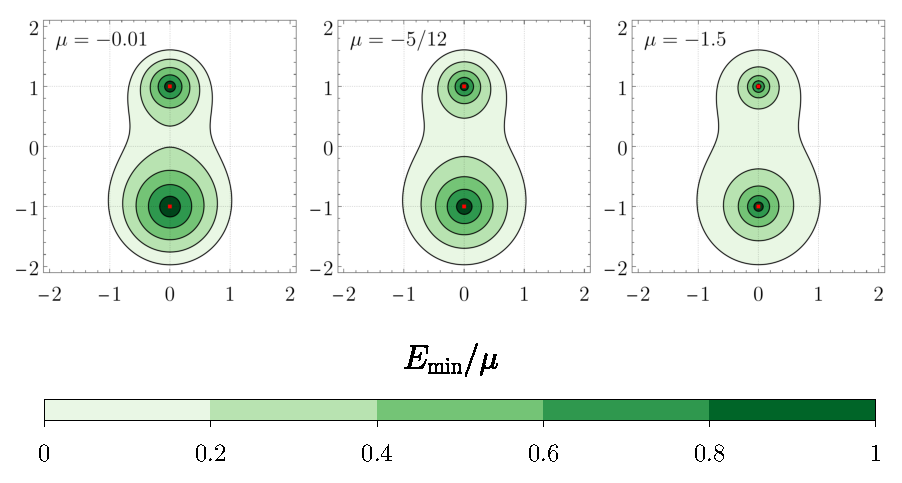
\includegraphics[width=\linewidth]{img/penrose_binaries/fig3.pdf}
  \caption{Energy levels inside the generalized ergosphere of a \ac{MP} black hole with $M_R=1/2$ and $\overline \mu = -5/4$, corresponding to the point \textbf{E} in Figs.~\ref{fig:regions} and \ref{fig:ergos}. The color bar represents $E_{\mathrm min}/\mu$. From left to right, the panels correspond respectively to $\mu=-0.01$, $\mu=-5/12$, and $\mu=-1.5$. The horizontal and vertical axes in each panel are $\overline \rho$ and $\overline z$, respectively. The red dots indicate the location of the black holes.}
  \label{fig:energylevels}
\end{figure}

The minimum energy (per unit mass) at a given point of the spacetime, in contrast, depends on the explicit values of $\mu$, $M_R$ and $M_T/a$. To illustrate this dependence, we plot in Fig.~\ref{fig:energylevels} the energy levels inside the ergosphere determined by $M_R=1/2$ and $\overline \mu = -5/4$ (which corresponds to the point \textbf{E} in Figs.~\ref{fig:regions} and \ref{fig:ergos}) for different combinations of $\mu$ and $M_T/a$. The color bar in Fig.~\ref{fig:energylevels} indicates the value of $E_{\mathrm{min}}/\mu$, which, according to Eq.~\eqref{eq:minimum_energy}, varies from zero (at the boundary of the ergosphere) to one (at the black holes). As $|\mu|$ decreases and $M_T/a$ increases (while $\overline \mu$ and $M_R$ are kept fixed), the shape of the ergosphere remains unchanged, but the energy levels become more evenly distributed around the black holes.

\subsection{Negative energy trajectories}
\label{sec:neg_energy}

Trajectories associated with negative energies are confined within the ergosphere defined by Eq.~\eqref{eq:rescaled_negative_energy_condition}. For a generic set of initial conditions, such paths will eventually end up at either one of the black holes. This is not much different from the case of a single RN or a Kerr black hole, in which particles with negative energies that start outside the event horizon necessarily enter the black hole and reach the spacetime singularity. Instead of focusing on this type of trajectory, we concentrated on trajectories which have no analogs in standard (Kerr and RN) black hole spacetimes~\cite{Grib:2013hxa,Zaslavskii:2020crn}. We want to investigate whether closed orbits of negative energy that live outside the black holes are allowed. It is important to first note, however, that if the Kerr black hole is immersed in an external magnetic field, closed orbits of negative energy are allowed outside the event horizon~\cite{PRASANA1982,FELICE2004}. We also note that stable circular orbits of negative energy exist around a Kerr naked singularity (and that the \ac{PP} can effectively take place using such orbits)~\cite{STUCHLIK1980}. We follow the procedure described in the last paragraph of section \ref{sec:motion} to solve the equations of motion. To simplify our work, we restrict our attention to two classes of planar motion (among the many possibilities of orbits around the binary) and show that, by fine-tuning the initial data, one is able to find closed orbits of negative energies in the \ac{MP} spacetime. These closed orbits of negative energies are unstable, in the sense that generic perturbations of the initial conditions result in trajectories that end at one of the black holes.

The first class of orbits assumes zero angular momentum ($L=0$) so that the trajectories are restricted to a plane that contains both black holes (here we choose the $\phi=0$ plane without loss of generality). For a given set of parameters $a$, $M_1$, $M_2$, $E$, and $\mu$, after fixing $\rho(0) = 0$ and $\dot{z}(0) = 0$, we fine tune the initial position $z(0)$. The initial value $\dot{\rho} (0)$ is determined from Eq.~\eqref{eq:alternative_expression_for_energy}. To illustrate, we show in Fig.~\ref{fig:orbit_closed_bh} two examples of eight-shaped orbits obtained with this scheme. The left panel of Fig.~\ref{fig:orbit_closed_bh} represents an orbit with energy (per unit mass) $E=-2/10$ and charge-to-mass ratio $\mu=-5$ for an equal mass \ac{MP} binary ($M_1=M_2=1$) with separation parameter $a=1$. The trajectory starts on the $z$-axis, at $z(0) = 5.314064237978...$ (fine-tuned). One complete revolution of the trajectory, with corresponding period of $\lambda \approx 22.64$, is shown. The right panel of Fig.~\ref{fig:orbit_closed_bh}, on the other hand, exhibits an orbit of $E=-2/10$ and $\mu=-5$ for a \ac{MP} binary with mass ratio $M_R=1/2$ ($M_1=2,M_2=1$) and separation parameter $a=1$. The trajectory starts on the $z$-axis, at $z(0) = 12.832155724084...$ (fine-tuned). One complete revolution of the trajectory, with corresponding period of approximately $\lambda \approx 43.28$, is shown.

\begin{figure}[!ht]
  \centering
  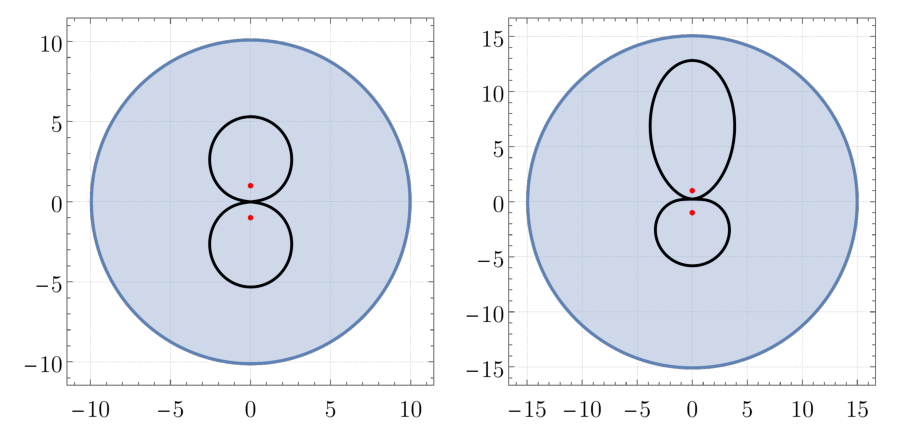
\includegraphics[width=\linewidth]{img/penrose_binaries/fig4.pdf}
  \caption{Example of closed trajectories of negative energy (black curves) in the plane containing the black holes. The blue region is the generalized ergosphere of the spacetime, while the red dots indicate the location of the black holes. The horizontal and vertical axes in each panel are $\overline \rho$ and $\overline z$, respectively. Left panel: trajectory corresponding to $L=0$, $E=-2/10$, $a=M_1=M_2=1$, $\mu = -5$, $\rho(0) = 0$, $z(0) = 5.314064237978...$ (fine-tuned), and $\dot{z}(0) = 0$. The associated period of revolution is $\lambda \approx 22.64$.  Right panel: trajectory corresponding to $L=0$, $E=-2/100$, $a=1$, $M_1=2 M_2= 2$, $\mu = -5$, $\rho(0) = 0$, $z(0) = 12.832155724084...$ (fine-tuned), and $\dot{z}(0) = 0$. The associated period of revolution is $\lambda \approx 43.28$. }
  \label{fig:orbit_closed_bh}
\end{figure}

The second class of orbits is only possible for equal mass binaries and comprises trajectories that are confined to the $z=0$ plane, which is the plane equidistant to the black holes. Particles with negative energy whose motion is constrained to this plane will evolve in a perpetual oscillatory motion, either in straight lines (when $L=0$) or in more complicated precessing orbits (when $L \neq 0$). Even though these trajectories are unstable to generic perturbations, on the plane itself they are stable. In other words, infinitesimal perturbations of $\rho(0)$ and $\dot \rho(0)$ produce infinitesimal variations on the original trajectory (if $z(0)$ and $\dot z(0)$ are kept fixed).

To analyze these orbits we resort to Eqs.~\eqref{eq:effective1}-\eqref{eq:effective3}. Given $a$, $E$ and $L$, the critical points $\rho$ where $E_{\mathrm{eff}}(\rho,0)^2 = V_{\mathrm{eff}}(\rho,0)$ represent circular closed orbits. Typically, however, the particle will be confined inside a compact section of the $z=0$ plane, in a characteristic ``zoom-whirl'' orbit~\cite{ASSUMPCAO2018,Levin:2008mq}, moving between a minimum radius $\rho_{\mathrm min}$ and a maximum radius $\rho_{\mathrm max}$. In Fig.~\ref{fig:orbit_closed_z}, we show the effective energy and the effective potential for a \ac{MP} spacetime with $a=1$ and $M_1 = M_2 = 1$, when the particle's charge-to-mass ratio, angular momentum (per unit mass), and energy (per unit mass) are, respectively, $\mu=-5$, $L=12.85869$, and $E=-5/100$. The particle is constrained to move between $\rho_{\mathrm min}\approx 0.543$ and $\rho_{\mathrm max}\approx 3.857$. The corresponding trajectory, assuming the starting point to be $\rho(0)=2$ and $\phi(0)=0$, is also shown in Fig.~\ref{fig:orbit_closed_z}.

\begin{figure}[!ht]
  \centering
  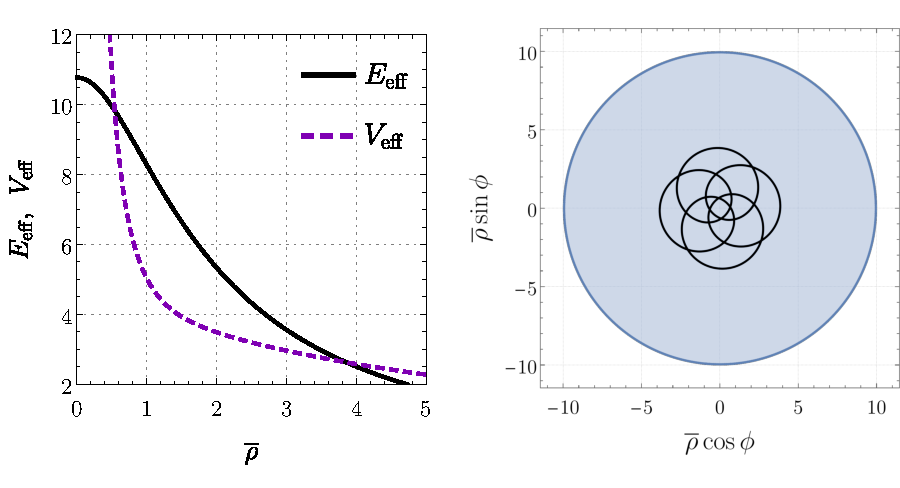
\includegraphics[width=\linewidth]{img/penrose_binaries/fig5.pdf}
  \caption{Left panel: effective energy (black curve) and effective potential (purple dashed curve) for $L=12.85869$, $E=-5/100$, $a=1$, $M_1 = M_2 = 1$, $\mu = -5$. Right panel: an example of a closed trajectory of negative energy in the $z = 0$ symmetry plane. The blue region is the generalized ergosphere of the spacetime. The trajectory (black curve) is generated by setting the parameters to $L=12.85869$, $E=-5/100$, $a=1$, $M_1 = M_2 = 1$, $\mu = -5$, $\rho(0) = 2$, and $\phi(0) = 0$. The associated period of revolution is $\lambda \approx 35$.}
  \label{fig:orbit_closed_z}
\end{figure}

\subsection{Penrose Process}

Following Penrose's original proposal~\cite{PENROSE1971} and its extension to RN black holes~\cite{RUFFINI1971,DENARDO1973}, we now investigate the possibility of energy extraction from a \ac{MP} binary black hole. The mechanism we shall explore is analogous to the most standard one: a negatively charged particle is sent towards the binary black hole and, once inside the generalized ergosphere, breaks up into two fragments, one of which escapes to infinity with more energy than the original particle. We assume that the incident particle follows a trajectory $T_{(0)}$, which starts outside the ergosphere and ends inside it, at the break-up point $(\rho_*,\phi_*,z_*)$. From the break-up point, two other trajectories, labeled $T_{(1)}$ and $T_{(2)}$, start. Each trajectory $T_{(i)}$ is a time-like path $x^{\mu}_{(i)}(\lambda)$ parametrized by its proper time $\lambda$. To fix notation, let $m_{(i)}$, $\mu_{(i)}$, $E_{(i)}$, $L_{(i)}$, and $P^{\mu}_{(i)}$ denote, respectively, the mass, the charge-to-mass ratio, the energy per unit mass, the angular momentum per unit mass (with respect to the z-axis), and the 4-momentum of the particle $i$ on trajectory $T_{(i)}$. We assume that fragment $1$ remains inside the ergosphere (meaning that $E_{(1)} < 0 $), while fragment $2$ escapes back to infinity.

The quantities that characterize each particle are related by conservation equations. Charge conservation, for instance, yields
\begin{equation}
  \mu_{(0)} m_{(0)}  = \mu_{(1)} m_{(1)} + \mu_{(2)} m_{(2)}.
  \label{eq:charge_conservation}
\end{equation}
The conservation of the four-momentum applied at the break-up point, on the other hand, reads
\begin{equation}
  P^{\mu}_{(0)} = P^{\mu}_{(1)} + P^{\mu}_{(2)}.
  \label{eq:four_momentum_conservation}
\end{equation}
Each component of the vector equation \eqref{eq:four_momentum_conservation} above corresponds to a different conservation equation with straightforward physical interpretation. The zero-component is just the conservation of total energy, i.e.
\begin{equation}
  E_{(0)}m_{(0)} = E_{(1)}m_{(1)} + E_{(2)}m_{(2)}.
  \label{eq:conservation_of_energy}
\end{equation}
The spatial components are the conservation of linear momenta, i.e.
\begin{equation}
  \begin{cases}
    m_{(0)}\dot{\rho}_{(0)} = m_{(1)}\dot{\rho}_{(1)} +m_{(2)}\dot{\rho}_{(2)} \\
    m_{(0)}\dot{z}_{(0)} = m_{(1)}\dot{z}_{(1)} + m_{(2)}\dot{z}_{(2)}
  \end{cases},
  \label{eq:conservation_mom_lin}
\end{equation}
and the conservation of angular momentum, i.e.
\begin{equation}
  L_{(0)}m_{(0)} = L_{(1)} m_{(1)} + L_{(2)}m_{(2)}.
  \label{eq:conservation_mom_ang}
\end{equation}
We remark that all derivatives in \eqref{eq:conservation_mom_lin} are evaluated at the break-up point. We also note that the break-up of the incident particle naturally imposes restrictions on the masses of its fragments. By squaring Eq.~\eqref{eq:four_momentum_conservation} and using the fact that the four-momentum is future-pointing and time-like, we obtain the inequality~\cite{bhat1985energetics}
\begin{equation} \label{eq:mass_constraint}
  m_{(1)}^2 + m_{(2)}^2 < m_{(0)}^2.
\end{equation}

\begin{figure}[!ht]
  \centering
  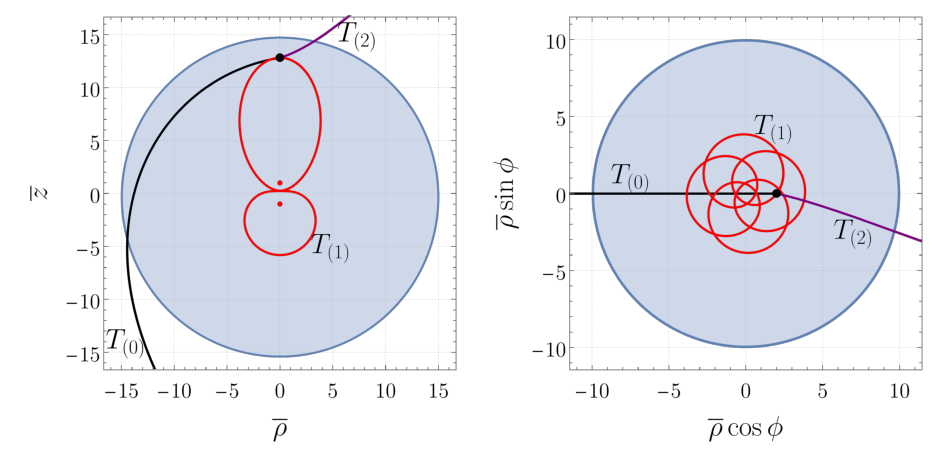
\includegraphics[width=\linewidth]{img/penrose_binaries/fig6.pdf}
  \caption{Left panel: \ac{PP} in the $\rho$-$z$ plane of a \ac{MP} spacetime with $M_1=2$, $M_2=1$, and $a=1$. Right panel: \ac{PP} in the $z=0$ plane of a \ac{MP} spacetime with $M_1=M_2=1$ and $a=1$. In each plot, the incoming trajectory $T_{(0)}$ (black curve) splits at the black point into the negative energy orbit $T_{(1)}$ (red curve) and the trajectory of the escaping fragment $T_{(2)}$ (purple curve). The parameters that generate these trajectories are shown in Tables \ref{tab:example1} and \ref{tab:example2}. The blue region is the generalized ergosphere (for particle 1) and the red dots indicate the location of the black holes.}
  \label{fig:example1}
\end{figure}

\begin{table}[h]
  \centering
  \begin{tabular}{ccccccc}
    \hline\hline
    $i$ & $m_{(i)}$ & $\mu_{(i)}$ & $E_{(i)}$ & $L_{(i)}$ & $\dot{\rho}_{(i)}$ & $\dot{z}_{(i)}$ \\ \vspace{-0.3cm} \\
    0   & 1.00000   & -0.08345    & 1.00000   & 0         & 0.60000            & 0.09699         \\
    1   & 0.70000   & -5.00000    & -0.02000  & 0         & 0.41207            & 0.00000         \\
    2   & 0.23248   & 14.69629    & 4.36171   & 0         & 1.34012            & 0.41719         \\
    \hline\hline
  \end{tabular}
  \caption{Parameters that generate the trajectories $T_{(0)}$, $T_{(1)}$, and $T_{(2)}$ of the \ac{PP} shown in the left panel of Fig.~\ref{fig:example1}. The derivatives $\dot{\rho}_{(i)}$ and $\dot{z}_{(i)}$ are evaluated at the break-up point.}
  \label{tab:example1}
\end{table}

\begin{table}[h]
  \centering
  \begin{tabular}{ccccccc}
    \hline\hline
    $i$ & $m_{(i)}$ & $\mu_{(i)}$ & $E_{(i)}$ & $L_{(i)}$ & $\dot{\rho}_{(i)}$ & $\dot{z}_{(i)}$ \\ \vspace{-0.3cm} \\
    0   & 1.00000   & -0.27698    & 1.00000   & 0.00000   & 1.00000            & 0               \\
    1   & 0.10000   & -5.00000    & -0.05000  & 12.85870  & 1.36059            & 0               \\
    2   & 0.33342   & 0.66890     & 3.01423   & -3.85662  & 2.59116            & 0               \\
    \hline\hline
  \end{tabular}
  \caption{Parameters that generate the trajectories $T_{(0)}$, $T_{(1)}$, and $T_{(2)}$ of the \ac{PP} shown in the right panel of Fig.~\ref{fig:example1}. The derivatives $\dot{\rho}_{(i)}$ and $\dot{z}_{(i)}$ are evaluated at the break-up point.}
  \label{tab:example2}
\end{table}

From Eq.~\eqref{eq:conservation_of_energy}, the energy carried away by the escaping fragment is $E_{(2)}m_{(2)} = E_{(0)}m_{(0)} - E_{(1)}m_{(1)}$. Since we have assumed that $E_{(1)} < 0$, the escaping particle will carry away more energy than the incident particle had. If the negative energy fragment collapses to one of the black holes, it will directly decrease the energy associated with the black hole, as in Penrose's original proposal. If, on the other hand, the negative energy fragment remains in a closed orbit (such as the ones described in Sec.~\ref{sec:neg_energy}), where does the extra energy for the escaping fragment come from? Since the final state (binary black hole and bound particle fragment) is less energetic than the binary itself, we conclude that the extracted energy is associated with the binding energy of the binary. In other words, the presence of the bound particle fragment reduces the energy required to form a \ac{MP} binary and the excess energy is transferred to the escaping fragment.


In Fig.~\ref{fig:example1} we exhibit examples of PPs that include some of the negative energy orbits shown in Sec.~\ref{sec:neg_energy}. The left panel exhibits a \ac{PP} that takes place in the $\rho$-$z$ plane of a \ac{MP} spacetime with $M_1=2$, $M_2=1$, and $a=1$. The incoming particle breaks-up at $\overline \rho=0$ and $\overline z = 5.314064237978...$ (fine-tuned). The right panel, on the other hand,  exhibits a \ac{PP} that occurs in the $z=0$ plane of a \ac{MP} spacetime with $M_1=M_2=1$ and $a=1$. The incoming particle breaks-up at $\overline \rho=2$ and $\phi = 0$. The parameters that generate these examples and satisfy Eqs.~\eqref{eq:charge_conservation}-\eqref{eq:mass_constraint} are given in Tables \ref{tab:example1} and \ref{tab:example2}.


\subsection{Energy extraction efficiency}

The efficiency $\eta$ of the \ac{PP} can be defined as the ratio between the energy output and the energy input. Using Eq.~\eqref{eq:conservation_of_energy}, we have
%%
\begin{equation}
  \eta = \frac{E_{(2)}m_{(2)} - E_{(0)}m_{(0)}}{E_{(0)}m_{(0)}} = - \frac{E_{(1)}m_{(1)}}{E_{(0)}m_{(0)}}.
  \label{eq:penrose_efficiency_general}
\end{equation}
%
A natural question arises: what is the maximum efficiency of the \ac{PP} in a \ac{MP} spacetime? Since $\eta$ is directly proportional to $E_{(1)}$ and inversely proportional to $E_{(0)}$, in order to maximize the efficiency of the process we need to make the absolute value of $E_{(1)}$ as large as possible and $E_{(0)}$ as small as possible. We also want the negative energy fragment to be as massive as possible in comparison to the mass of the incident particle. In other words, we want to extract as much energy as possible starting with as little energy as possible. We shall assume that the \ac{MP} spacetime is fixed (meaning that $M_1$, $M_2$ and $a$ are known), the break-up point has been specified as $(\rho_*, z_*, \phi_*)$ and the charge-to-mass ratio $\mu_{(1)}$ is known. Given these hypotheses, we will determine how much energy can be extracted from a \ac{MP} black hole and how the remaining parameters must be chosen in order to optimize the process.

First, the minimum energy for an incident particle coming from infinity, according to Eq.~\eqref{eq:alternative_expression_for_energy}, is $E_{(0)}=1$ and corresponds to the particle having zero kinetic energy at infinity. For that reason, we shall assume from now on that $L_{(0)}=0$ and $E_{(0)}=1$. Secondly, according to Eq.~\eqref{eq:minimum_energy} and the discussion in the first paragraph of Sec.~\ref{Sec:gen_ergo}, the energy per unit mass of particle $1$ is most negative if the particle is initially at rest. Therefore, at the break-up point we set
\begin{equation} \label{eq:traj1}
  \dot{\rho}_{(1)}=\dot{z}_{(1)}=\dot{\phi}_{(1)}=0,
\end{equation}
meaning that the associated angular momentum per unit mass and energy per unit mass are, respectively, $L_{(1)}=0$ and
\begin{equation} \label{eq:penrose_neg_energy}
  E_{(1)}=E_{(1)}^{\mathrm {min}}=\mu_{(1)}\left(1 - \frac{1}{U_*} \right) + \frac{1}{U_*},
\end{equation}
where we have defined $U_*=U(\rho_*,z_*)$ for simplicity.

Let us now study the allowed values for $m_{(1)}$. The conservation of linear momenta, Eq.~\eqref{eq:conservation_mom_lin}, yields the relation
\begin{equation} \label{eq:mass2_eq1}
  m_{(2)}^2  = m_{(0)}^2 \left( \frac{\dot \rho_{(0)} ^2 +  \dot z_{(0)} ^2 }{\dot \rho_{(2)} ^2 + \dot z_{(2)} ^2 } \right) + m_{(1)}^2 \left( \frac{\dot \rho_{(1)} ^2 + \dot z_{(1)} ^2 }{\dot \rho_{(2)} ^2 + \dot z_{(2)} ^2 } \right),
\end{equation}
where all derivatives are evaluated at the break-up point.
After replacing $\dot \rho_{(i)} ^2 + \dot z_{(i)} ^2$ using Eqs.~\eqref{eq:effective1}-\eqref{eq:effective3}, and employing the conservation equations  \eqref{eq:charge_conservation}, \eqref{eq:conservation_of_energy} and \eqref{eq:conservation_mom_ang}, the expression above reduces to
\begin{equation} \label{eq:mass2_eq2}
  m_{(2)} = \sqrt{m_{(0)}^2 - 2 m_{(0)} m_{(1)} \alpha_{(0)} + m_{(1)}^2},
\end{equation}
where
\begin{equation} \label{eq:alpha_definition}
  \alpha_{(0)} =  U_* \left[ 1 - \mu_{(0)}\left(1 - \frac{1}{U_*}\right) \right].
\end{equation}
Note that the expression between brackets in the definition of $\alpha_{(0)}$ is precisely the effective energy of the incident particle evaluated at the break-up point as given by Eq.~\eqref{eq:effective2}. The inequalities given in Eq.~\eqref{eq:effective_constraints}, together with the fact that $U_* \ge 1$, therefore imply that
\begin{equation} \label{eq:alpha_constraint}
  \alpha_{(0)} \ge 1,
\end{equation}
and
\begin{equation} \label{eq:mu0max}
  \mu_{(0)} \le 1.
\end{equation}

Eq.~\eqref{eq:mass2_eq2} and the fact that the masses are positive, together with the constraint imposed by Eq.~\eqref{eq:mass_constraint}, also imply that
\begin{equation}\label{eq:bound_of_m1_m0}
  0 < \frac{m_{(1)}}{m_{(0)}} < \alpha_{(0)} .
\end{equation}
%\le \sqrt{1 + \frac{L_0^2}{\rho_*^2 U_*^2}}
Since the radicand in Eq.~\eqref{eq:mass2_eq2} must be positive, the bound given by Eq.~\eqref{eq:bound_of_m1_m0} can be further refined to yield
\begin{equation} \label{eq:m1_max}
  0 < m_{(1)} < m_{(0)} \left( \alpha_{(0)} - \sqrt{\alpha_{(0)}^2 - 1} \right).
\end{equation}
Hence, the allowed range for $m_{(1)}$ is maximized when the inequalities \eqref{eq:alpha_constraint} and \eqref{eq:mu0max} are saturated. In fact, when $\mu_{(0)} \rightarrow 1$ one can choose $m_{(1)}\rightarrow m_{(0)}$, thus maximizing the ratio $m_{(1)}/m_{(0)}$ that appears in Eq.~\eqref{eq:penrose_efficiency_general}. Consequently, the efficiency of the \ac{PP} in a \ac{MP} spacetime is bound from above according to
\begin{equation} \label{eq:eta_max_theory}
  \eta < \eta ^{b}  = -E_{(1)}^{\mathrm {min}}.
\end{equation}
%
We remark that the upper bound above is a function of $\mu_{(1)}$, the break-up point coordinates $\rho_*$ and $z_*$, and the \ac{MP} parameters ($M_1$, $M_2$, and $a$). With the help of Eq.~\eqref{eq:penrose_neg_energy}, we now investigate in detail how these quantities affect the efficiency bound.

The dependence of $\eta^{b}$ on the charge-to-mass ratio $\mu_{(1)}$ is simple: $\eta^{b}$ increases linearly with $\mu_{(1)}$. The dependence of $\eta^{b}$ on the break-up point can be understood with the help of the energy levels shown in Fig.~\ref{fig:energylevels}: the efficiency bound increases as the break-up point approaches either one of the black holes. A more detailed analysis is shown in Fig.~\ref{fig:efficiency0}, where we plot $\eta^{b}$ as a function of $z_*$ for selected values of $\rho_*$ when $M_R=1/2$, $M_T=3$, and $\overline \mu_{(1)} = -5/4$ (corresponding to the energy levels shown in the middle panel of Fig.~\ref{fig:energylevels}). Note that when the break-up point is outside the ergosphere, the efficiency bound becomes negative, meaning that the escaping fragment will carry away less energy than the incident particle had. The \ac{PP} is most efficient if the break-up occurs exactly at either one of the event horizons, as indicated by the red dots in Fig.~\ref{fig:efficiency0}. When this happens, the upper bound is $-\mu_{(1)}$, which is in agreement with results obtained for the RN metric~\cite{bhat1985energetics,parthasarathy1986high}.

\begin{figure}[!ht]
  \centering
  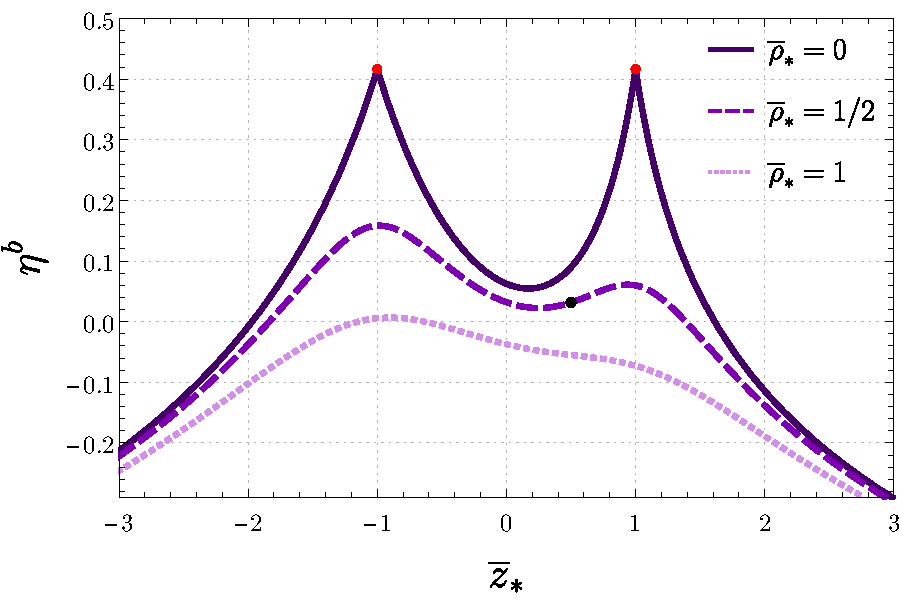
\includegraphics[width=\linewidth]{img/penrose_binaries/fig7.pdf}
  \caption{Efficiency bound $\eta ^ b$ as a function of $z_*$ for $\overline \rho_*=0$ (solid curve), $\overline \rho_*=1/2$ (dashed curve), and $\overline \rho_*=1$ (dotted curve) when $M_R=1/2$, $M_T=3$, and $\overline \mu_{(1)} = -5/4$. The associated ergosphere corresponds to the point \textbf{E} in Figs.~\ref{fig:regions} and \ref{fig:ergos}, while the associated energy levels are shown in the middle panel of Fig.~\ref{fig:energylevels}. The red dots indicate the efficiency when the particle breaks-up at the black holes. The black dot shows the maximum efficiency $\eta^b = 0.03161$ for the processes represented in Fig.~\ref{fig:examplemax1} and Tables \ref{tab:max1} and \ref{tab:max2}.}
  \label{fig:efficiency0}
\end{figure}

To study the dependence of the efficiency bound on the masses of the black holes, we plot $\eta ^{b}$ as a function of the mass ratio $M_R$ when $M_T/a=3$ (top panel of Fig.~\ref{fig:efficiency2}) and as a function of $M_T/a$ when $M_R=1/2$  (top panel of Fig.~\ref{fig:efficiency3}). In both cases we have set the charge-to-mass ratio as $\mu_{(1)} = -5/12$. Each curve in these plots is associated with a different break-up point. The break-up points are shown in the bottom panels of Figs.~\ref{fig:efficiency2} and \ref{fig:efficiency3}. In the bottom panel of Fig.~\ref{fig:efficiency2}, we also exhibit the generalized ergosphere associated with a few selected values of $M_R$ (which are chosen to reproduce the ergospheres labeled \textbf{D}, \textbf{E} and \textbf{F} in Figs.~\ref{fig:regions} and \ref{fig:ergos}). Analogously, the ergospheres depicted in the bottom panel of Fig.~\ref{fig:efficiency3} (and the associated values of $M_T/a$) correspond to the ergospheres labeled \textbf{B}, \textbf{E} and \textbf{H} in Figs.~\ref{fig:regions} and \ref{fig:ergos}.

As shown in the top panel of Fig.~\ref{fig:efficiency2}, when the mass ratio $M_R$ increases (while the other parameters are kept fixed), $\eta ^{b}$ will also increase if the break-up point is closer to the lighter black hole and will decrease if the break-up point is closer to the heavier black hole. This behavior is related to the fact that the growth of $M_R$ produces an expansion of the ergosphere around the lighter companion and a reduction of the ergosphere around the heavier companion, as seen in the bottom panel of Fig.~\ref{fig:efficiency2}.
Note that the efficiency bound is independent of the mass ratio if the break-up point is equidistant to the black holes.
On the other hand, as shown in Fig.~\ref{fig:efficiency3}, when $M_T/a$ increases (while the other parameters are kept fixed), the ergosphere expands and $\eta ^{b}$ increases. We note that in the limit $M_T/a \rightarrow \infty$, no matter where the break-up occurs, the efficiency bound approaches its maximum, i.e. $\eta ^{b} \rightarrow - \mu_{(1)}$. This is explained by the fact that the distance between the break-up point and the black holes becomes negligible in comparison to the size of the ergosphere when $M_T/a \rightarrow \infty$.

\begin{figure}[!ht]
  \centering
  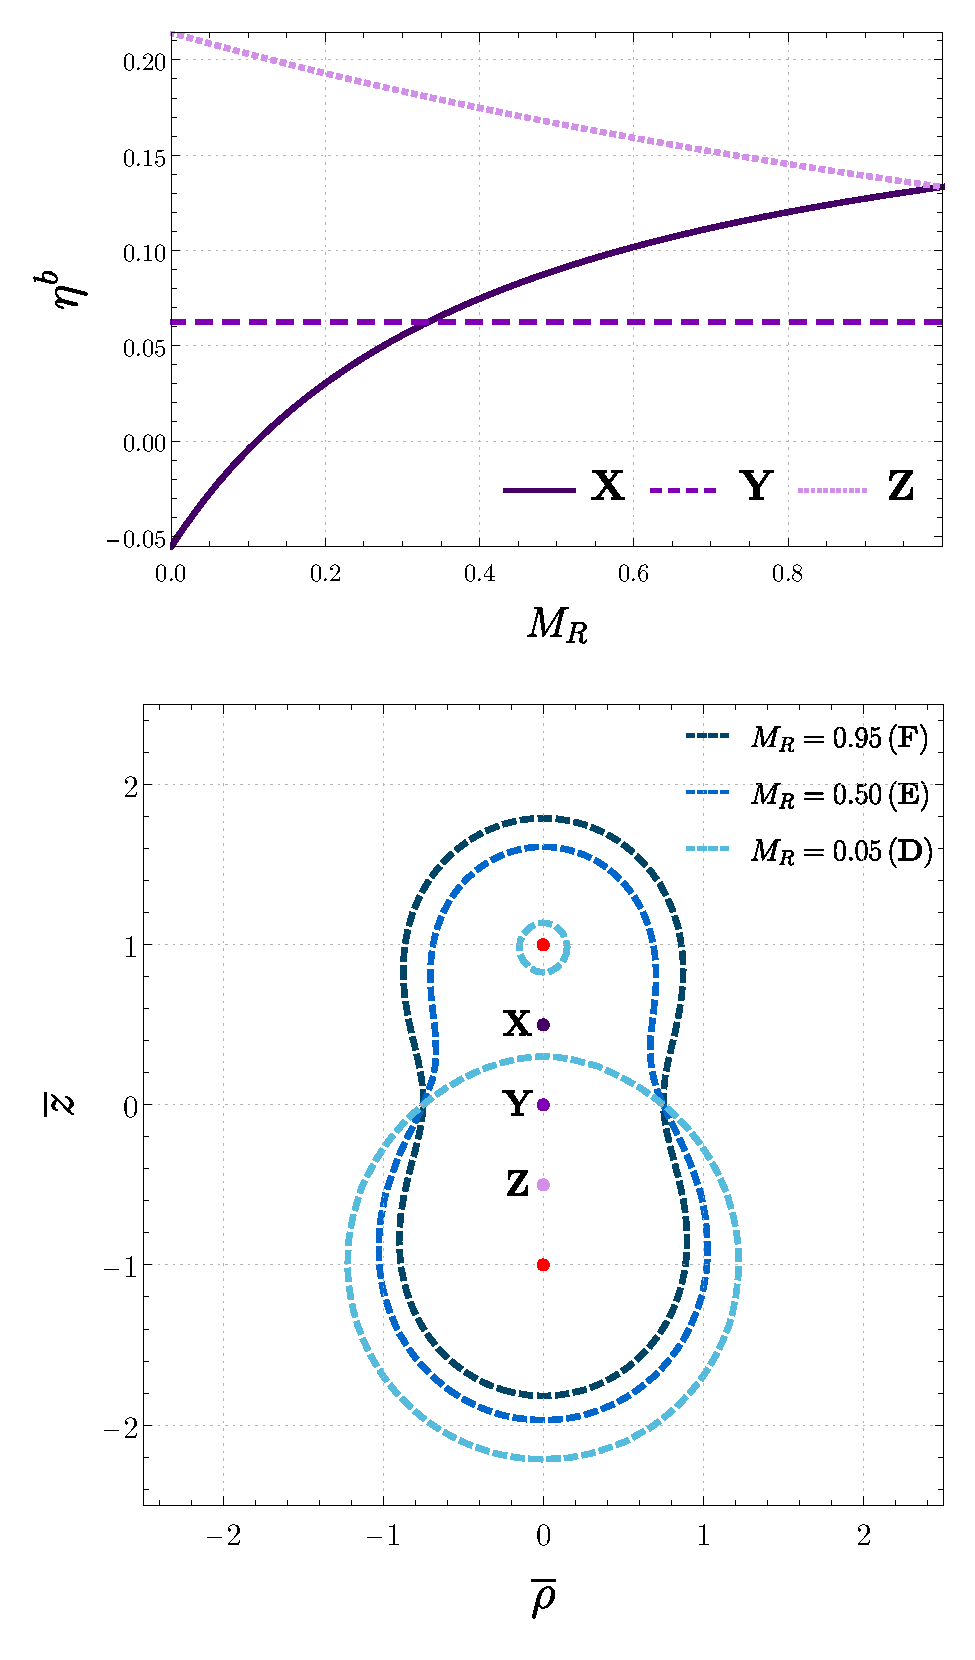
\includegraphics[scale=0.5]{img/penrose_binaries/fig8.pdf}
  \caption{Top panel: efficiency bound $\eta^{b}$ as a function of $M_R$ when $M_T/a=3$ and $\mu_{(1)} = -5/12$. Bottom panel: generalized ergosphere for selected values of $M_R$ (corresponding to the points  \textbf{D}, \textbf{E} and \textbf{F} in Fig.~\ref{fig:regions}) when $M_T/a=3$ and $\mu_{(1)} = -5/12$. The red dots indicate the location of the black holes. The purple dots are the locations of the break-up points $(\overline \rho_*,\overline z_*)=(1/2,1/2)$, $(\overline \rho_*,\overline z_*)=(1/2,0)$, and $(\overline \rho_*,\overline z_*)=(1/2,-1/2)$ and are labeled \textbf{X}, \textbf{Y} and \textbf{Z}, respectively. Each curve in the top panel corresponds to one of the break-up points shown in the bottom panel.}
  \label{fig:efficiency2}
\end{figure}

Finally, we investigate the behavior of $\eta ^{b}$ when $\mu_{(1)}$ and $M_T/a$ vary simultaneously, but their product, i.e. $\overline \mu_{(1)} = \mu_{(1)} M_T/a$, is kept fixed, meaning that the shape of the ergosphere is fixed (only the energy levels inside it change). In Fig.~\ref{fig:efficiency1} we plot $\eta^b$ as a function of $\mu_{(1)}$ and $M_T/a$ for three different break-up points when $M_R=1/2$ and $\overline \mu_{(1)} = -5/4$, so that the resulting ergosphere corresponds to the one labeled \textbf{E} in Figs.~\ref{fig:regions} and \ref{fig:ergos}. The break-up points are chosen to be $(\overline \rho_*,\overline z_*)=(d,1-d)$, with $d=1/2$, $d=1/3$, and $d=1/4$. We observe that, as $|\overline {\mu}|$ increases and $M_T/a$ decreases, the efficiency bound increases, approaching an asymptotic value in the limit $\mu_{(1)} \rightarrow -\infty$ and $M_T/a \rightarrow 0$.

\begin{figure}[!ht]
  \centering
  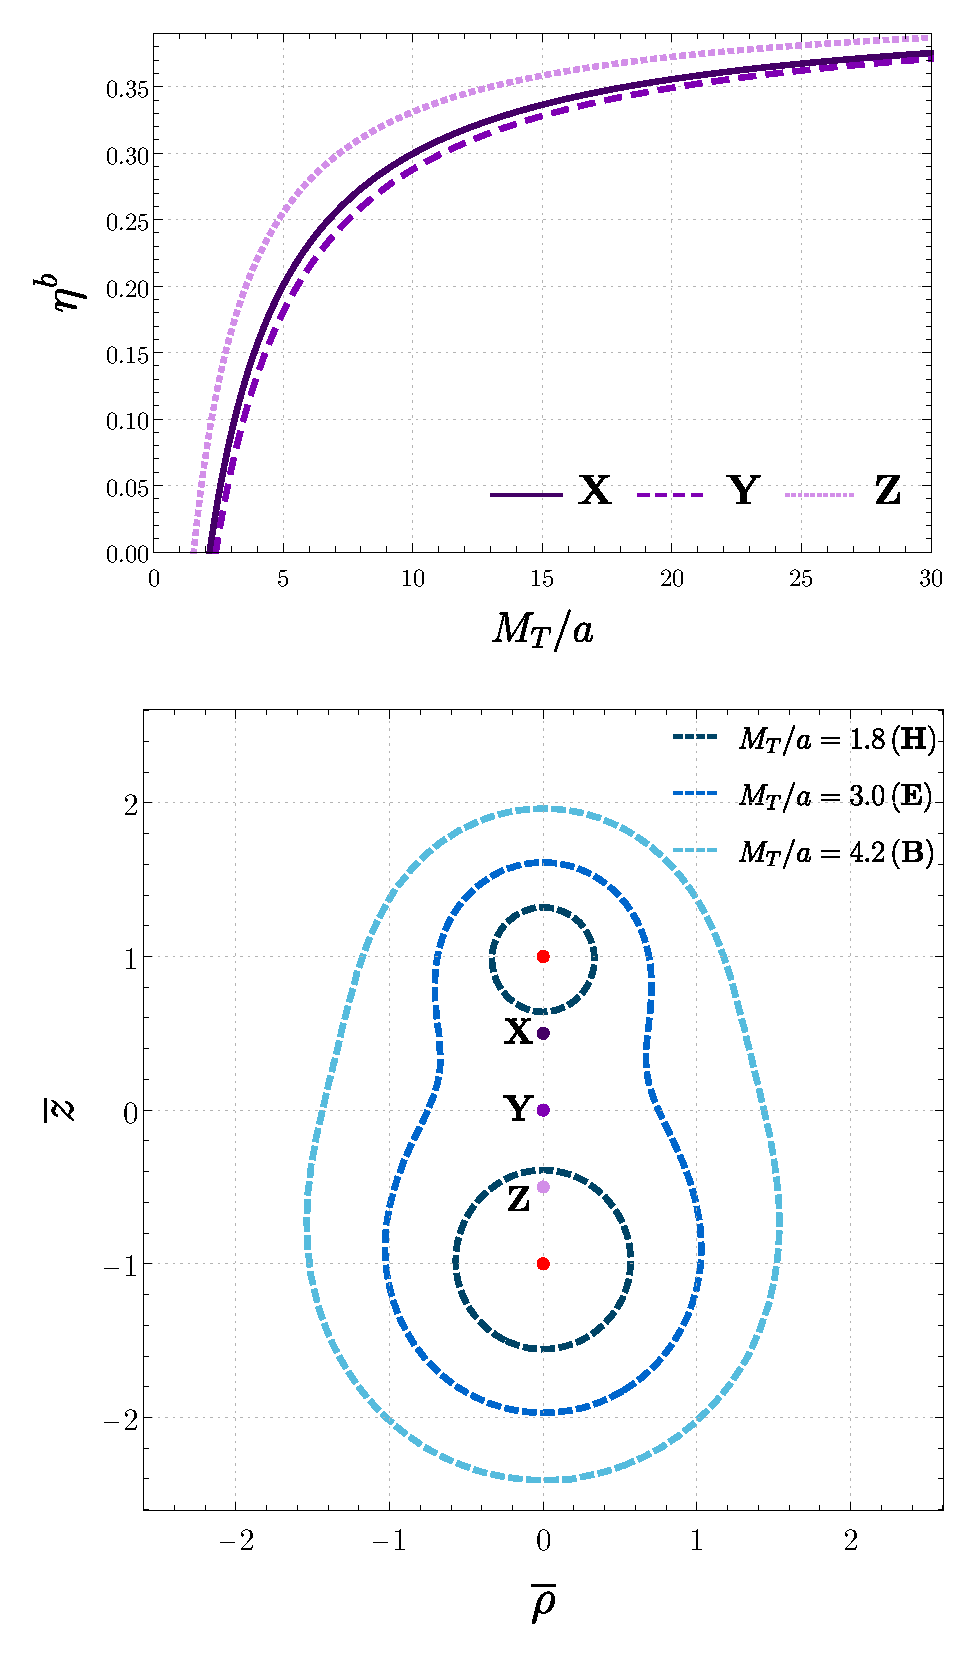
\includegraphics[scale=0.5]{img/penrose_binaries/fig9.pdf}
  \caption{Top panel: efficiency bound $\eta^{b}$ as a function of $M_T/a$ when $M_R=1/2$ and $\mu_{(1)} = -5/12$. Bottom panel: generalized ergosphere for selected values of $M_T/a$ (corresponding to the points  \textbf{B}, \textbf{E} and \textbf{H} in Fig.~\ref{fig:regions}) when $M_R=1/2$ and $\mu_{(1)} = -5/12$. The red dots indicate the location of the black holes. The purple dots are the locations of the break-up points $(\overline \rho_*,\overline z_*)=(1/2,1/2)$, $(\overline \rho_*,\overline z_*)=(1/2,0)$, and $(\overline \rho_*,\overline z_*)=(1/2,-1/2)$ and are labeled \textbf{X}, \textbf{Y} and \textbf{Z}, respectively. Each curve in the top panel corresponds to one of the break-up points shown in the bottom panel.}
  \label{fig:efficiency3}
\end{figure}

\begin{figure}[!ht]
  \centering
  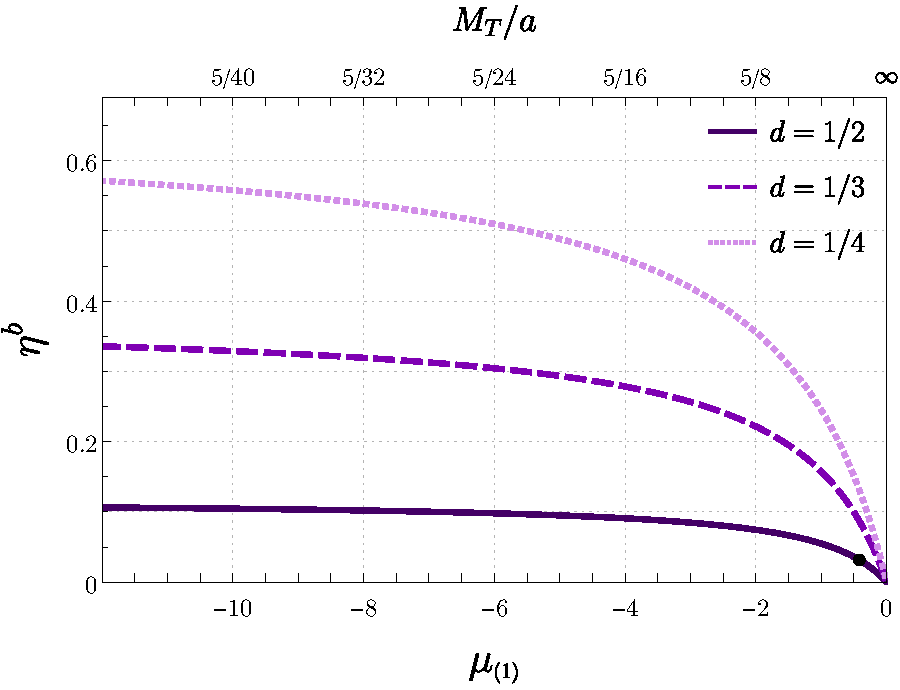
\includegraphics[width=\linewidth]{img/penrose_binaries/fig10.pdf}
  \caption{Efficiency bound $\eta ^ b$ as a function of $\mu_{(1)}$ (bottom axis) and $M_T/a$ (top axis) for $M_R=1/2$ and $\overline \mu _{(1)} = -5/4$. The fact that $\overline \mu _{(1)}$ is fixed implies that $\mu_{(1)}$ and $M_T/a$ are inversely proportional to each other. The curves, from bottom to top, correspond to the break-up points $(\overline \rho_*, \overline z_*)=(d,1-d)$, with $d=1/2$, $d=1/3$, and $d=1/4$ respectively. The black dot shows the maximum efficiency $\eta^b = 0.03161$ for the processes represented in Fig.~\ref{fig:examplemax1} and Tables \ref{tab:max1} and \ref{tab:max2}, i.e.~when $d=1/2$, $\mu_{(1)} = - 5/12$ and $M_T/a=3$.}
  \label{fig:efficiency1}
\end{figure}

\subsection{Examples}

We now give concrete examples of energy extraction in a \ac{MP} binary black hole spacetime whose efficiency approaches the theoretical maximum given by Eq.~\eqref{eq:eta_max_theory}. The general procedure that we follow is outlined below. First, we choose the \ac{MP} parameters $M_1$, $M_2$ and $a$. Second, we choose the charge-to-mass ratio $\mu_{(1)}$ and a break-up point $(\rho_*,z_*,\phi_*)$ that is inside the generalized ergosphere of the spacetime. Without loss of generality, we set $m_{(0)}=1$.

Following the discussion leading to the inequality \eqref{eq:eta_max_theory}, we set $L_{(0)}=L_{(1)}=L_{(2)}=0$, meaning that all trajectories are restricted to the plane $\phi=\phi_*$. The energy $E_{(1)}$ is determined by Eq.~\eqref{eq:penrose_neg_energy}, while $E_{(0)}=1$. According to Eqs.~\eqref{eq:mu0max} and \eqref{eq:m1_max}, we choose
\begin{eqnarray}
  \label{eq:epsilondef} \mu_{(0)} &= 1 - \varepsilon, \\
  \label{eq:nudef} m_{(1)} &= 1 - \nu,
\end{eqnarray}
where $\varepsilon$ and $\nu$ are small positive parameters satisfying
\begin{equation} \label{eq:nuepsilonrelation}
  \nu > \varepsilon (U_* - 1) \left( \sqrt{1 + \frac{2}{\varepsilon (U_* - 1)}} - 1 \right).
\end{equation}
Since $m_{(1)}$  has been fixed, the mass $m_{(2)}$ can be determined by Eq.~\eqref{eq:mass2_eq2}. The quantities $\mu_{(2)}$ and $E_{(2)}$ are determined from Eqs.~\eqref{eq:charge_conservation} and \eqref{eq:conservation_of_energy}, respectively.

At the break-up point, according to Eq.~\eqref{eq:traj1}, we have $\dot \rho_{(1)}=\dot z_{(1)} = 0$ for the negative energy fragment. For the incident particle, on the other hand, the choices for $\mu_{(0)}$ and $E_{(0)}$ imply that
%
\begin{equation}\label{eq:velocity_eq_max_energy_example}
  \dot \rho_{(0)} ^2 + \dot z_{(0)} ^2 = \varepsilon \frac{U_*-1}{U_* ^2} \left[2 + \varepsilon (U_* - 1) \right].
\end{equation}
%
By choosing the angle $\theta_{(0)} = \mathrm{Arg}\left(\dot \rho_{(0)} + i \, \dot z_{(0)} \right)$ between the velocities $\dot \rho_{(0)}$ and $\dot z_{(0)}$, equation Eq.~\eqref{eq:velocity_eq_max_energy_example} can be used to determine $\dot \rho_{(0)}$ and $\dot z_{(0)}$ individually at the break-up point. The conservation of linear momentum then fixes the values of $\dot \rho_{(2)}$ and $\dot z_{(2)}$ through Eq.~\eqref{eq:conservation_mom_lin}. At this point, the trajectories $T_{(0)}$, $T_{(1)}$, and $T_{(2)}$ have all been determined and the efficiency of the associated \ac{PP} is $\eta=(1-\nu)\eta^{b}$.  In order to maximize the efficiency of the \ac{PP}, one must, therefore, set $\eta$ to be as small as possible. Note, however, that one cannot choose $\varepsilon=0$, because this would imply $\dot \rho_{(0)} = \dot z_{(0)} = 0$ and  $\ddot \rho_{(0)} = \ddot z_{(0)} = 0$ at the break-up point, contradicting the fact the trajectory $T_{(0)}$ starts infinitely far away. Similarly, $\nu$ cannot be chosen to saturate inequality \eqref{eq:nuepsilonrelation}, otherwise $m_{(2)}$ would be exactly zero, contradicting the fact that all trajectories are time-like. If desired, this can be remedied by assuming, from the start, that the escaping fragment is massless (however, this would modify Eq.~\eqref{eq:alternative_expression_for_energy} and the present analysis). Nevertheless, it is possible, in principle, to have infinitesimally small values for $\varepsilon$ and $\nu$. Finally, we point out that not every angle $\theta_0$ produces trajectories that are consistent with the assumptions of a \ac{PP}. More precisely, only certain ranges of $\theta_0$ give rise to trajectories  $T_{(0)}$ and $T_{(2)}$ that, respectively, start and end infinitely far away from the black holes.

\begin{figure}[!ht]
  \centering
  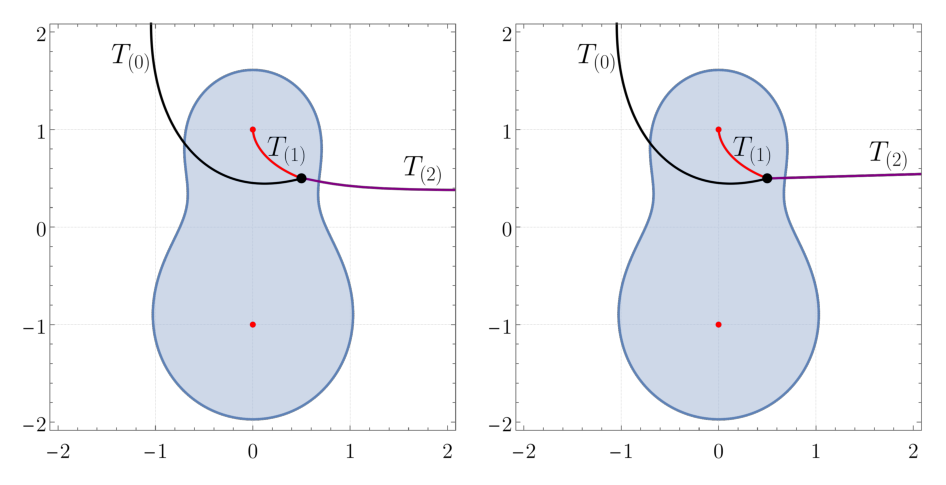
\includegraphics[width=\linewidth]{img/penrose_binaries/fig11.pdf}
  \caption{Examples of PPs that approach the maximum theoretical efficiency in a \ac{MP} spacetime. The efficiencies of the processes in the left and right panel are, respectively, $90 \%$ and $99 \%$ of the theoretical maximum. In both cases the incoming trajectory $T_{(0)}$ (black curve) splits at the black point into the negative energy orbit $T_{(1)}$ (red curve) and the trajectory of the escaping fragment $T_{(2)}$ (purple curve). The parameters that generate these trajectories are shown in Tables \ref{tab:max1} and \ref{tab:max2}. The blue region is the generalized ergosphere (for particle 1) and the red dots indicate the location of the black holes.}
  \label{fig:examplemax1}
\end{figure}

\begin{table}[h]
  \centering
  \begin{tabular}{ccccccc}
    \hline\hline
    $i$ & $m_{(i)}$ & $\mu_{(i)}$ & $E_{(i)}$ & $L_{(i)}$ & $\dot{\rho}_{(i)}$ & $\dot{z}_{(i)}$ \\ \vspace{-0.3cm} \\
    0   & 1.00000   & 0.99990     & 1.00000   & 0         & 0.00609            & 0.00158         \\
    1   & 0.90000   & -0.41667    & -0.03161  & 0         & 0.00000            & 0.00000         \\
    2   & 0.09756   & 14.09301    & 10.54183  & 0         & 0.06243            & 0.01621         \\
    \hline\hline
  \end{tabular}
  \caption{Parameters that generate the trajectories $T_{(0)}$, $T_{(1)}$, and $T_{(2)}$ of the \ac{PP} shown in the left panel of Fig.~\ref{fig:examplemax1}. The derivatives $\dot{\rho}_{(i)}$ and $\dot{z}_{(i)}$ are evaluated at the break-up point.
  }
  \label{tab:max1}
\end{table}

\begin{table}[h]
  \centering
  \begin{tabular}{ccccccc}
    \hline\hline
    $i$ & $m_{(i)}$ & $\mu_{(i)}$ & $E_{(i)}$ & $L_{(i)}$ & $\dot{\rho}_{(i)}$ & $\dot{z}_{(i)}$ \\ \vspace{-0.3cm} \\
    0   & 1         & 0.99999     & 1.00000   & 0         & 0.00193            & 0.00050         \\
    1   & 0.99000   & -0.41667    & -0.03161  & 0         & 0.00000            & 0.00000         \\
    2   & 0.00685   & 206.13521   & 150.50460 & 0         & 0.28104            & 0.07297         \\
    \hline\hline
  \end{tabular}
  \caption{Parameters that generate the trajectories $T_{(0)}$, $T_{(1)}$, and $T_{(2)}$ of the \ac{PP} shown in the right panel of Fig.~\ref{fig:examplemax1}. The derivatives $\dot{\rho}_{(i)}$ and $\dot{z}_{(i)}$ are evaluated at the break-up point.
  }
  \label{tab:max2}
\end{table}

We conclude by showing in Fig.~\ref{fig:examplemax1} two explicit examples of the procedure outlined above for the \ac{MP} spacetime with $M_1=2$, $M_2=1$, and $a=1$. The charge-to-mass ratio of the negative energy fragment is chosen as $\mu_{(1)}=-5/12$, so that the associated generalized ergosphere is the one identified by the letter \textbf{E} in Figs.~\ref{fig:regions} and \ref{fig:ergos}. The  break-up point is chosen as $(\rho_*,z_*)=(1/2,1/2)$, fixing the trajectory $T_{(1)}$ and its energy (per unit mass) $E_{(1)}=-0.03161$ (remember that the initial conditions are chosen so that $E_{(1)}$ is the minimum possible). According to Eq.~\eqref{eq:eta_max_theory}, the efficiency bound is $\eta^{b} = 0.03161$ (which corresponds to the black dots in Figs.~\ref{fig:efficiency0} and \ref{fig:efficiency1}). The trajectories $T_{(0)}$ and $T_{(2)}$ are specified by the choices of $\varepsilon$, $\nu$, and $\theta_{(0)}$. In the left panel of Fig.~\ref{fig:examplemax1}  we exhibit the \ac{PP} for $\varepsilon=10^{-4}$, $\nu=10^{-1}$, and $\theta_{(0)}=0.25403$, whose efficiency is $90 \%$ of the theoretical maximum. In the right panel of Fig.~\ref{fig:examplemax1} we exhibit the \ac{PP} for $\varepsilon=10^{-5}$, $\nu=10^{-2}$, and $\theta_{(0)}=0.25403$, whose efficiency is $99 \%$ of the theoretical maximum. The parameters that generate these examples and satisfy Eqs.~\eqref{eq:charge_conservation}-\eqref{eq:mass_constraint} are  given in Tables \ref{tab:max1} and \ref{tab:max2}.

\section{CMMR Spacetime}
\label{ch:penrose_binaries:sec:cmmr_penrose}
We now consider the extension of the results presented in Sec.~\ref{ch:penrose_binaries:sec:mp_penrose} to a binary system of rotating black holes described by the CMMR metric. In Weyl's cylindrical coordinates, the CMMR line element reads
%
\begin{multline}
  \ud s^2 = -f(\rho,z)\left[\ud t - \omega(\rho,z)\ud\phi\right]^2 \\
  + f(\rho,z)^{-1}\left[e^{2\gamma(\rho,z)}\left(\ud \rho^2 + \ud z^2\right) + \rho^2\ud\phi^2\right],
  \label{eq:cmmr_line_element}
\end{multline}
%
where the real valued functions $f(\rho,z)$, $\omega(\rho,z)$ and $\exp[2\gamma(\rho,z)]$ are defined as in Sec.~IV of Ref.~\cite{manko_ruiz_thermo}. As in the case of the MP metric, only the exterior of the black holes is described by these coordinates. In particular, the outer event horizons of the constituent black holes are straight lines in these coordinates (see Fig.~\ref{fig:cmmr_ergospheres}).

The CMMR solution is fully characterized by five independent parameters, namely the masses $M_{1,2}$, the angular momenta per unit mass $a_{1,2}$ and the coordinate distance $R$ between the black hole centers. From these, we define three additional parameters, namely $M_T = M_1 + M_2$, which represents the total mass of the system, $J_T = M_1 a_1 + M_2 a_2$, which represents the total angular momentum of the system, and $a_*$, which is a root of the cubic equation
%
\begin{equation}
  \left(R^2 - M_T^2 + a_*^2\right) \left(a_1 + a_2 - a_*\right) + 2 \left(R + M_T \right)\left(J_T - M_T a_* \right) = 0.
  \label{eq:cubic_eq_for_a}
\end{equation}

We note that, depending on the parameters, the CMMR metric can represent a black hole-black hole binary, a naked singularity-naked singularity binary, or a black hole-naked singularity binary~\cite{cabrera_metric,manko_ruiz_metric, manko_ruiz_thermo}. In our analysis, the chosen parameters always correspond to a binary black hole solution. In practice, this means that the chosen parameters must:
%
\begin{enumerate}
  \item Produce real valued and positive horizon lengths. The horizon half-lengths are given by the expressions $\sigma_1$ and $\sigma_2$ in Sec.~IV of Ref.~\cite{manko_ruiz_thermo}.
  \item Produce horizons that do not touch or overlap.
  \item Produce a single real root for $a_*$ in Eq.~\eqref{eq:cubic_eq_for_a}.
\end{enumerate}

\subsection{Geodesics}

Once again, we will make use of the Lagrangian formalism to determine the geodesic equations and the conserved quantities corresponding to the symmetries of the system. The Lagrangian associated with the geodesic motion of a massive and neutral test particle in the CMMR metric is~\cite{Dubeibe2016}
%
\begin{equation}
  2\mathcal{L} = -f(\dot{t} - \omega\dot{\phi})^2 +f^{-1}\left[e^{2\gamma}\left( \dot{\rho}^2 + \dot{z}^2 \right) + \rho^2\dot{\phi}^2 \right],
  \label{eq:cmmr_lagrangian}
\end{equation}
where, once again, dots represent derivatives with respect to the proper time $\lambda$.

%
Due to the stationarity and the axisymmetry of the system, we can identify two constants of the motion analogous to the quantities defined in Eqs.~\eqref{eq:conserved_energy}  and \eqref{eq:conserved_momentum}. The energy per unit mass, as measured by a static observer at infinity, is given by
%
\begin{equation}
  E = f\dot{t} - \omega f\dot{\phi},
  \label{eq:cmmr_energy_t_phi}
\end{equation}
%
and the angular momentum (with respect to the $z$ axis) per unit mass, as measured by a static observer at infinity, is given by
%
\begin{equation}
  L = \omega f \dot{t} + \left( \frac{\rho^2}{f} - \omega^2 f \right)\dot{\phi}.
  \label{eq:cmmr_ang_mom_t_phi}
\end{equation}
%

Using Eqs.~\eqref{eq:cmmr_energy_t_phi} and \eqref{eq:cmmr_ang_mom_t_phi} to eliminate $\dot{t}$ and $\dot{\phi}$ from the normalization of the four velocity, i.e. $\dot{x}^\mu\dot{x}_\mu = -1$, we obtain an expression for the energy $E$ in  terms of $\dot{\rho}$, $\dot{z}$ and the angular momentum $L$:
%
\begin{equation}
  E  = \frac{-f^2\omega L}{\rho^2-\omega^2 f^2}  + \left[ \frac{\rho^2e^{2\gamma}(\dot{\rho}^2 + \dot{z}^2)}{\rho^2 - \omega^2f^2} + \left( \frac{\rho fL}{\rho^2 - \omega^2f^2} \right)^2 + \frac{\rho^2f}{\rho^2 - \omega^2f^2} \right]^{1/2},
  \label{eq:cmmr_energy_rho_z}
\end{equation}
%
where the positive sign is once again chosen for the square root in order to guarantee that a static particle at infinity has positive energy. We rewrite the equation above as Eq.~\eqref{eq:effective1}, where the effective energy and the effective potential are now given by
%
\begin{equation}
  V_{\text{eff}} = \frac{\rho^2 - \omega^2 f^2}{\rho^2 e^{2\gamma}}\left[ \left( \frac{\rho fL}{\rho^2 - \omega^2f^2} \right)^2 + \frac{\rho^2f}{\rho^2 - \omega^2f^2}\right]
  \label{eq:cmmr_effective_potential}
\end{equation}
%
and
%
\begin{equation}
  E_{\text{eff}} = \frac{\rho^2 - \omega^2 f^2}{\rho^2 e^{2\gamma}}\left(E + \frac{f^2\omega L}{\rho^2-\omega^2 f^2}\right)^2.
  \label{eq:cmmr_effective_energy}
\end{equation}
%
%
Note that the constraints given in Eq.~\eqref{eq:effective_constraints} also apply to Eqs.~\eqref{eq:cmmr_effective_potential} and \eqref{eq:cmmr_effective_energy}.

The geodesic equations, analogous to Eqs.~\eqref{eq:ode_for_rho_motion} and \eqref{eq:ode_for_z_motion}, can be derived from the Euler-Lagrange equations for the Lagrangian \eqref{eq:cmmr_lagrangian}. Their explicit forms, in terms of $E$, $L$ and the metric functions $f$, $\omega$ and $e^{2\gamma}$, are given in Eqs.~(16) and (17) of Ref.~\cite{Dubeibe2016}. Once $\rho(\lambda)$ and $z(\lambda)$ are known, $t(\lambda)$ and $\phi(\lambda)$ are determined by direct integration of Eqs.~\eqref{eq:cmmr_energy_t_phi} and \eqref{eq:cmmr_ang_mom_t_phi}.


\subsection{Ergosphere}

Since the CMMR metric is stationary, and we are considering neutral particles in geodesic motion, we use the standard definition of an ergosphere to study the possibility of negative energy orbits and energy extraction. In other words, the ergosphere is the region where the time translation Killing vector field becomes space-like, i.e.~$(\partial_t)^\mu (\partial_t)_\mu > 0$. Taking into account the line element \eqref{eq:cmmr_line_element}, it is straightforward to show that the ergosphere of the CMMR spacetime is the locus of points that satisfy
%
\begin{equation}
  f(\rho,z) < 0.
  \label{eq:cmmr_ergo_ineq}
\end{equation}

We sketch this ergosphere in Fig.~\ref{fig:cmmr_ergospheres}, where each panel is labeled by a letter (\textbf{A}-\textbf{I}) and corresponds to a different set of parameters (which are specified in Table \ref{tab:cmmr_ergo_tab}). In each panel, the blue shaded region represents the $\phi = 0$ section of the ergosphere, while the red lines represent the event horizons of the black holes. The top row of the figure (panels \textbf{A}-\textbf{C}) exhibits the effect of changing the mass ratio of the system while keeping the total mass, both spins and the separation parameter fixed. It shows that, analogously to the MP case, initially disjoint ergospheres may merge into a single connected ergosphere when the mass ratio increases. The middle row of Fig.~\ref{fig:cmmr_ergospheres} (panels \textbf{D}-\textbf{E}), on the other hand, shows the effect of changing the spin parameter of the top black hole while keeping all other parameters fixed. We observe that when initially aligned spins become anti-aligned, the ergosphere becomes thinner and elongated along the symmetry axis. Finally, the bottom row (panels \textbf{G}-\textbf{H}) illustrates the effect of increasing the separation parameter when all other parameters are kept fixed. Similarly to what happens in the MP case, if the distance between the black holes is sufficiently large, there will be two disconnected ergospheres, one for each black hole.

\begin{figure}[!ht]
  \centering
  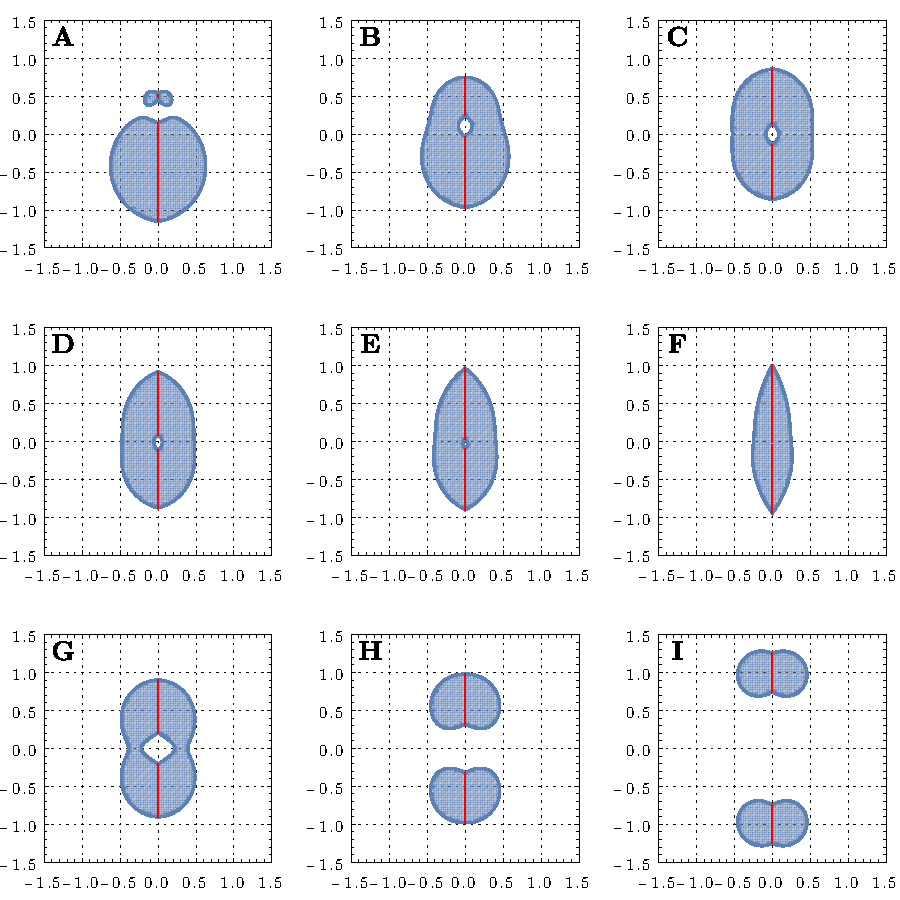
\includegraphics[width=\linewidth]{img/penrose_binaries/fig12.pdf}
  \caption{The $\phi=0$ section of the ergosphere of the CMMR metric for different set of parameters labeled \textbf{A}-\textbf{I} (see Table  \ref{tab:cmmr_ergo_tab}). In each plot the horizontal and vertical axes are $\rho/M_T$ and $z/M_T$, respectively. The red lines indicate the location of the black hole's horizons.}
  \label{fig:cmmr_ergospheres}
\end{figure}

\begin{table}[h]
  \centering
  \begin{tabular}{ccccc}
    \hline\hline
    Panel      & $M_1/M_2$ & $a_1/M_T$ & $a_2/M_T$ & $R/M_T$ \\
    \textbf{A} & $0.16$    & $0.65$    & $0.65$    & $1.00$  \\
    \textbf{B} & $0.58$    & $0.65$    & $0.65$    & $1.00$  \\
    \textbf{C} & $1.00$    & $0.65$    & $0.65$    & $1.00$  \\
    \textbf{D} & $1.00$    & $0.50$    & $0.65$    & $1.00$  \\
    \textbf{E} & $1.00$    & $0.30$    & $0.65$    & $1.00$  \\
    \textbf{F} & $1.00$    & $-0.10$   & $0.65$    & $1.00$  \\
    \textbf{G} & $1.00$    & $0.65$    & $0.65$    & $1.11$  \\
    \textbf{H} & $1.00$    & $0.65$    & $0.65$    & $1.30$  \\
    \textbf{I} & $1.00$    & $0.65$    & $0.65$    & $2.00$  \\
    \hline\hline
  \end{tabular}
  \caption{Parameters that define the CMMR metrics associated with the ergospheres \textbf{A}-\textbf{I} shown in Fig.~\ref{fig:cmmr_ergospheres}.}
  \label{tab:cmmr_ergo_tab}
\end{table}


\subsection{Bound negative energy orbits and the PP}

To demonstrate the existence of bound negative energy orbits and the possibility of using them to extract energy from non-coalescing Kerr binaries, we shall restrict our attention to systems of equal mass and spin. This symmetry allows for the existence of stable orbits (in the sense already discussed for the MP metric) in the $z=0$ plane. To find a negative energy trajectory that is confined outside the black holes, we choose the energy $E$ and the angular momentum $L$ such that there are two orbital turning points of Eq.~\eqref{eq:effective1} that lie inside the ergosphere of the system. Similarly to what was done in the MP case, once the initial radius $\rho(0)$, the energy, and the angular momentum are fixed, we solve Eq.~\eqref{eq:cmmr_energy_rho_z} to determine $\dot{\rho}(0)$ and integrate the geodesic equations. Using the parameters that produce the ergosphere \textbf{C} of Fig.~\ref{fig:cmmr_ergospheres} and Table \ref{tab:cmmr_ergo_tab}, we show an example of such a negative energy orbit in Fig.~\ref{fig:cmmr_veff} (right panel). The corresponding effective potential and effective energy are also shown in Fig.~\ref{fig:cmmr_veff} (left panel).

\begin{figure}[!ht]
  \centering
  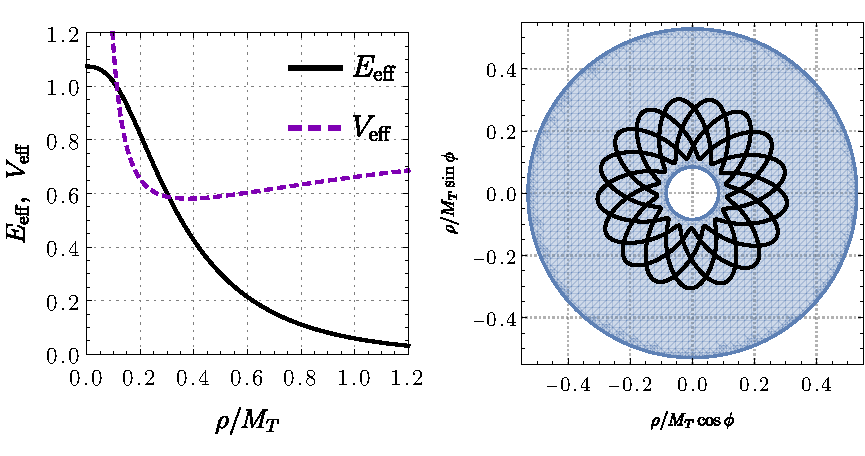
\includegraphics[width=\linewidth]{img/penrose_binaries/fig13.pdf}
  \caption{Left panel: effective energy (black curve) and effective potential (purple dashed curve) for $L=-2.5$ and $E=-0.054$, when the CMMR metric is characterized by $a_1=a_2=0.65$, $M_1 = M_2 = 0.5$, and $R = 1$ (corresponding to the label \textbf{C} in Table \ref{tab:cmmr_ergo_tab}). The turning points are located at $\rho_{-}/M_T = 0.112531$ and at $\rho_{+}/M_T = 0.306081$. Right panel: the associated trajectory in the $z = 0$ plane when $\rho(0)/M_T=0.25$ and $\phi(0)=0$. The blue region is the $z=0$ section of the ergosphere of the spacetime.}
  \label{fig:cmmr_veff}
\end{figure}

Adopting the same notation introduced Sec.~\ref{ch:penrose_binaries:sec:mp_penrose} for the trajectories in a PP around the MP black hole, and taking advantage of the negative energy orbit depicted in Fig.~\ref{fig:cmmr_veff}, we now consider the possibility of energy extraction in the CMMR spacetime. By employing the conservation of 4-momentum (as in Sec.~III), we construct an explicit example of a PP. The obtained trajectories are shown in Fig.~\ref{fig:cmmr_penrose} and the corresponding parameters are given in Table \ref{tab:cmmr_penrose_example}. The efficiency of the process, calculated through Eq.~\eqref{eq:penrose_efficiency_general}, is $\eta \approx 0.08 \%$.

\begin{figure}[!ht]
  \centering
  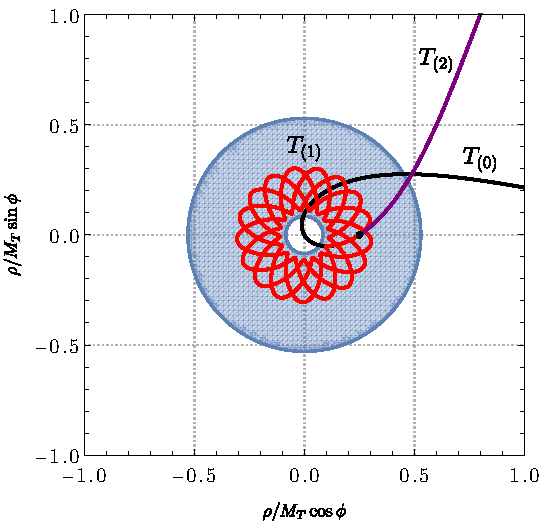
\includegraphics[width=\linewidth]{img/penrose_binaries/fig14.pdf}
  \caption{Penrose's process in the $z=0$ plane of a CMMR spacetime with $M_1=M_2=0.5$, $a_1=a_2=0.65$, and $R=1$. The incoming trajectory $T_{(0)}$ (black curve) splits at the black point ($\rho/M_T=0.25$, $\phi=0$) into the negative energy orbit $T_{(1)}$ (red curve) and the trajectory of the escaping fragment $T_{(2)}$ (purple curve). The parameters that generate these trajectories are shown in Table \ref{tab:cmmr_penrose_example}. The blue region is the $z=0$ section of the ergosphere (for particle 1).}
  \label{fig:cmmr_penrose}
\end{figure}

\renewcommand{\arraystretch}{1.2}
\begin{table}[h]
  \centering
  \begin{tabular}{ccccccc}
    \hline\hline
    $i$ & $m_{(i)}/m_0$ & $E_{(i)}$ & $L_{(i)}$         & $\dot{\rho}_{(i)}$ & $\dot{z}_{(i)}$ \\ \vspace{-0.3cm} \\
    0   & 1.0000000     & 2.00000   & 0         .000000 & 4.343904           & 0               \\
    1   & 0.0289697     & -0.05400  & -2.500000         & 0.313887           & 0               \\
    2   & 0.3148980     & 6.35623   & 0.229993          & 13.765800          & 0               \\
    \hline\hline
  \end{tabular}
  \caption{Parameters that generate the trajectories $T_{(0)}$, $T_{(1)}$, and $T_{(2)}$ of the PP shown in Fig.~\ref{fig:cmmr_penrose}. The derivatives $\dot{\rho}_{(i)}$ and $\dot{z}_{(i)}$ are evaluated at the break-up point.}
  \label{tab:cmmr_penrose_example}
\end{table}

\section{Arbitrary Spacetimes}
\label{ch:penrose_binaries:sec:arbitrary_penrose}
In the previous sections, all of our considerations depended upon the existence of a conserved negative and ``global'' (as seen by a static observer at infinity) energy. This is only possible if the spacetime under consideration is stationary. 

In this section we will demonstrate how one can still observe the PP even in cases where this assumption is relaxed and there is no global and conserved energy available to be explored, thus, looking only at locally defined quantities. This technique allows one to study the Penrose mechanism even when the spacetime metric is defined numerically, such as is the case in numerical simulations of binary black hole collisions.

\subsection{3+1 split of the geodesic equation}

To understand our proposed technique, it is first fundamental to understand how General Relativity can be reformulated by explicitly separating its spatial and temporal components. This decomposition know as a ``3+1 split'' is very commonly used in Numerical Relativity and was motivated by the first attempts of posing GR as a Cauchy problem. Numerical Relativity codes very often provide ways to access the spacetime metrics being evolved in terms of its 3+1 components.

In this section, we will assume familiarity of the reader with this concept which can be readily reviewed in Refs.~\cite{Alcubierre2012-xp, 9780521514071, 9781108928250}. Given that the PP requires us to investigate the trajectories of particles in a background spacetime, we must now solve the geodesic equation taking into account that the spacetime metric (and its derivatives) will be provided via 3+1 split components. 

The need to solve the geodesic equation in this context overlaps with works that are interested in simulating an image of a black hole, that is, determining what a camera would capture if it was pointed towards a black hole. In this type of simulation a technique called \emph{backwards ray tracing} is employed, which consists in choosing a position and orientation of a model camera and integrating the trajectory of the photons that hit the camera's ``film'' backwards in time. In the event that the photon is assimilated by the system, the corresponding pixel within the image will appear black. If the photon ``collides'' with an obstacle such as a distant star or even an artificially colored background, the hue of the pixel is equivalent to the hue of that specific obstacle.

In spite of divergent objectives, the mathematical instruments utilized in backwards ray tracing are integral to the procedure that will imminently be formulated. The exhaustive and intricate derivation of the 3+1 decomposition of the geodesic equation utilized in this segment can be located in Ref.~\cite{Vincent_2012}. The terminologies and notions that are required for the development of our proposal will be derived from this source. 

Initially, we consider a globally hyperbolic spacetime that can be characterized by a metric tensor $\mtrtens{\mu}{\nu}$. Since it is globally hyperbolic, it allows for a foliation of constant coordinate time $t$ hypersurfaces that can be specified as $\Sigma_t$. We shall assume that the spacetime is equipped with coordinates\footnote{Our convention entails that Greek indices encompass all four coordinates, whereas Latin indices include only spatial coordinates.} that are adapted to the foliation, such that $x^0=t$ and $x^i$ ranges over $\Sigma_t$.

The unit time-like (directed towards the future) normal vector of $\Sigma_t$ shall be identified as $n^\mu$. This vector coincides with the four-velocity of an observer, known as the \emph{Eulerian Observer} or $\mathcal{O}E$, whose worldlines are orthogonal to $\Sigma_t$. The spatial metric induced in $\Sigma_t$ is designated as $\gamma{\mu\nu}$, and its associated covariant derivative is $D_i$. The extrinsic curvature tensor is $K_{ij}$, the lapse function is $N$, and the shift vector is $\beta^\mu$. The line element of the $3+1$ decompose metric then becomes
%
\begin{equation}
  \ud s^2 = -N^2 \ud t^2 + \gamma_{ij}(\ud x^i + \beta^i \ud t)(\ud x^j + \beta^j \ud t).
  \label{eq:arbitrary_penrose_decomposed_metric}
\end{equation}

Let us now consider a particle $\mathcal{P}$ of 4-momentum $p^\mu$. Let us assume that the particle moves in either a time-like or null geodesic (and thus without the influence of any force but gravity), which implies that
%
\begin{equation}
  p_\mu p^\mu = m^2\delta,
  \label{eq:arbitrary_penrose_p_norm}
\end{equation}
% 
where $\delta = -1$ for massive particles (and in this case $m$ represents the particle's mass) or $\delta=0$ for photons. The 4-momentum can be decomposed as
%
\begin{equation}
  p^\mu = E(n^\mu + V^\mu)
  \label{eq:arbitrary_penrose_p_decomp}
\end{equation}
%
where $E$ represents the particle's energy as measured by $\mathcal{O}_E$ (by definition,  $E = - n_\mu p^\mu$) and $V^\mu$ represents the 3-velocity of the particle, also as measured by $\mathcal{O}_E$. The 3-momentum $P^\mu$ of $\mathcal{P}$ as observed by $\mathcal{O}_E$ is thus
%
\begin{equation}
  P^\mu \equiv \tens{\gamma}{\mu}{\nu} p^\nu = E V^\mu.
  \label{eq:arbitrary_penrose_3_momentum}
\end{equation}
%
The normalization of $p^\mu$ and $n_\mu$, together with the orthogonality relation $n_\mu V^\mu = 0$ and Eq.~\eqref{eq:arbitrary_penrose_p_decomp} imposes
%
\begin{equation}
  V_\mu V^\mu = V_i V^i  = 1 + \delta\left(\frac{m}{E}\right)^2.
  \label{eq:arbitrary_penrose_V_norm}
\end{equation}
%
Finally, parametrizing the particle's position vector $X^i$ by the coordinate time (that is $x^i = X^i(t)$) the geodesic equation of $\mathcal{P}$ is decomposed in a set of 7 equations, namely
%
\begin{align}
  \der{X^i}{t} & = N V^i - \beta^i \label{eq:arbitrary_penrose_geodesic_eq_X}                                                                                                                                                  \\
  \der{V^i}{t} & = N V^j\left[ V^i \left( \partial_j \ln N - K_{jk} V^k \right) + 2 \tens{K}{i}{j} - {}^3\Gamma^{i}_{jk}V^k\right] - \gamma^{ij}\partial_j N - V^j\partial_j\beta^i \label{eq:arbitrary_penrose_geodesic_eq_V} \\
  \der{E}{t}   & = E (N K_{jk} V^j V^k - V^j \partial_j N) \label{eq:arbitrary_penrose_geodesic_eq_E}
\end{align}
%
where ${}^3\Gamma^{i}_{jk}$ are the Christoffel symbols associated with $\gamma_{ij}$.

\subsection{Penrose process}

Henceforth, $E$ shall be designated as the \emph{local energy}, given that it is gauged locally by the observer that is orthogonal to the foliation (the Eulerian Observer). In Sections~\ref{ch:penrose_binaries:sec:penrose_review}-\ref{ch:penrose_binaries:sec:cmmr_penrose}, we have been addressing what shall henceforth be referred to as the \emph{global energy}, i.e., the energy measured by a static observer stationed at infinity, which we shall now denote by $\varepsilon$. Our investigation necessitates the establishment of a connection between these two quantities, and we shall proceed to do so at this point. The global energy, $\varepsilon$ is defined as
%
\begin{equation}
  \varepsilon = - p_\mu \xi^\mu.
  \label{eq:arbitrary_penrose_global_energy_def}
\end{equation}
%
where $\xi^\mu = (\partial_t)^\mu$.
%
Expanding the contraction in Eq.~\eqref{eq:arbitrary_penrose_global_energy_def} with the general metric given in Eq.~\eqref{eq:arbitrary_penrose_decomposed_metric} and with the 4-momentum given in Eq.~\eqref{eq:arbitrary_penrose_p_decomp}, we get
%
\begin{equation}
  \varepsilon = \left( N - \gamma_{ij} \beta^i V^j \right) E.
  \label{eq:arbitrary_penrose_local_global_energy_relation}
\end{equation}

It is noteworthy that in the event that $\xi^\mu$ denotes a global time-like killing vector field pertaining to the background spacetime metric, $\varepsilon$ emerges as a conserved quantity along a particle's trajectory. As previously demonstrated, this fact was utilized to determine whether energy was extracted as an outcome of a particle disintegration process by evaluating the global energies of the particles implicated, one of which was necessarily characterized by a negative energy value. Due to the invariance of $\varepsilon$ along the particle's trajectories, the timing and location of this comparison were irrelevant.

If we, however, relax the assumption that the $\xi^\mu$ is a global time-like killing vector field, the quantity given by Eq.~\eqref{eq:arbitrary_penrose_global_energy_def} is no longer physically meaningful as an energy measure, thus restricting all physical arguments to be made in terms of local energy $E$ measurements. Furthermore, local energy, as can be explicitly seen in Eq.~\eqref{eq:arbitrary_penrose_geodesic_eq_E}, is not in general conserved along the particle's trajectory and must always be positive in order to be physically meaningful.


Given the aforementioned constraints, how can the local energies of particles engaged in a collision or a breakup process be compared in a physically significant manner to determine whether the system has lost or gained energy? To resolve this issue, it is essential to consider a crucial implication of Eq.~\eqref{eq:arbitrary_penrose_local_global_energy_relation}, which is that if the spacetime metric is asymptotically flat, meaning it becomes the Minkowski solution at an infinitely remote distance from the black hole (or holes), a significant inference can be derived.

In the limit where spatial coordinates approach infinity, the components of the spatial metric $\gamma_{ij}$ approach those of the Minkowski metric $\eta_{ij}$, the shift vector $\beta^i$ approaches zero, and the lapse function $N$ approaches one. Therefore, according to Eq.~\eqref{eq:arbitrary_penrose_local_global_energy_relation}, the global energy $\varepsilon$ and the local energy $E$ coincide at infinity. This means that if the spacetime is asymptotically flat, the global energy is still physically meaningful at infinity. Moreover, Eq.~\eqref{eq:arbitrary_penrose_geodesic_eq_E} implies that $K_{ij}$ approaches zero and $N$ approaches one as the Minkowski solution is approached, so both global and local energies are conserved at infinity.

In practical terms (and especially when analyzing spacetime metrics obtained from numerical simulation codes) it is not possible to integrate a trajectory to spatial infinity since the coordinates commonly employed are not compactified and such compactification schemes are often difficult or impossible to perform in practice.

Instead of attempting to do so, our technique follows again a practice common in backward ray tracing works, more specifically, we follow the prescription given by Ref.~\cite{Bohn:2014xxa}. Given a set of initial conditions $X^i(0), V^i(0), E(0)$, we evolve the system formed by Eqs.~\eqref{eq:arbitrary_penrose_geodesic_eq_X}-\eqref{eq:arbitrary_penrose_geodesic_eq_E} numerically until the particle reaches a sphere of predetermined radius that we denominate the \emph{background sphere}. The radius of this sphere is chosen so that the difference between global and local energy becomes smaller than a certain threshold $\delta_E$, that is, 
%
\begin{equation}
  |E(t_f)- \varepsilon(t_f)| < \delta_E,
  \label{eq:arbitrary_penrose_background_sphere_cplision_condition}
\end{equation}
%
where $t_f$ represents the final integration coordinate time. Additionally, we also stop integrating if the particle is absorbed by the system at a given time of ``swallowing'' $t_S$. A particle is considered absorbed if the difference of its local energy at $t_S$ and at $t=0$ gets larger than a certain swallowing threshold $\delta_S$, that is, 
%
\begin{equation}
  |E(t_S) - E(0)|/E(0) = \delta_S.
  \label{eq:arbitrary_penrose_swallowing_condition}
\end{equation}

The scheme described above was implemented in a public \texttt{C++} code available in Ref.~\cite{GRLensingRepo}. Compilation and usage instructions are provided within the repository. See Appendix~\ref{app:grlensing} for further information.

\subsection{Parametrizing initial velocities}

As was previously mentioned, we must choose 7 parameters in order to solve the 3+1 split geodesic equation. Once initial positions $X^i(0)$ and local energy $E(0)$ values are chosen one is still free to choose 3 initial velocity $V^i(0)$ values. We have chosen to consider only orbits in the $z=0$ plane, which implies $V^3(0)=0$. We do not believe that this choice represents a loss of generality since it is valid for all cases of interest, including astrophysical black hole binaries. By comparing Eq.~\eqref{eq:arbitrary_penrose_V_norm} to a general bi-variate quadratic form
%
\begin{equation}
  A X^2 + 2 B X Y + C Y^2 + 2 D X + 2 F Y + G = 0,
  \label{eq:arbitrary_penrose_general_quadratic_form}
\end{equation}
%
it is possible to identify
%
\begin{equation}
  A = \gamma_{22},\, B = \gamma_{23},\, C = \gamma_{33},\, G = -\left[ 1 - \left( \frac{m}{E} \right)^2 \right],\, D = F = 0,
\end{equation}
%
and the variables $X$ and $Y$ with $V^1$ and $V^2$, respectively. This quadratic describes a non-degenerate real ellipse in the $V^1$-$V^2$ plane centered around $V^1_\circ$ and $V^2_\circ$ with semi-axis lengths $\alpha_\pm$ and counterclockwise angle $\phi$ of rotation from the $V^1$ axis to its semi-major axis if after defining~\cite{Hart2002}
%
\begin{equation}
  \Delta = 
  \begin{vmatrix}
    A & B & D  \\
    B & C & F  \\
    D & F & G
  \end{vmatrix}
  = \left( 1 - \left( \frac{m}{E} \right)^2 \right) \left(\gamma_{23}^2-\gamma_{22} \gamma_{33}\right)
  \label{eq:arbitrary_penrose_quadratic_determinant}
  ,
\end{equation}
%
\begin{equation}
  J = 
  \begin{vmatrix}
    A & B \\
    B & C \\
  \end{vmatrix}
  = \gamma_{22} + \gamma_{33} - \gamma_{23}^2
  \label{eq:arbitrary_penrose_quadratic_J}
\end{equation}
%
and
%
\begin{equation}
  I = A + C = \gamma_{22} + \gamma_{33},
  \label{eq:arbitrary_penrose_quadratic_I}
\end{equation}
%
one has $\Delta \neq 0$, $J > 0$, $\Delta/I < 0$ and $\gamma_{22} \neq \gamma_{33}$. Explicitly, we have~\cite{Larson2006, Young2010, Lawrence2014}
%
\begin{equation}
  V^1_\circ = V^2_\circ = 0,
  \label{eq:arbitrary_penrose_ellipse_centers}
\end{equation}
%
\begin{equation}
  \alpha_\pm = \sqrt{ \frac{2 \left( 1 - \left(m/E\right)^2 \right)}{\gamma_{22} \mp \sqrt{4 \gamma_{23}^2 + \left( \gamma_{22} - \gamma_{33} \right)^2} +\gamma_{33}} }
  \label{eq:arbitrary_penrose_ellipse_axis}
\end{equation}
%
and
\begin{equation}
  \phi =
  \begin{cases}
    0                                                                                                 & \text{if } \gamma_{23} = 0 \text{ and } \gamma_{22} < \gamma_{33}    \\
    \frac{\pi}{2}                                                                                     & \text{if } \gamma_{23} = 0 \text{ and } \gamma_{22} > \gamma_{33}    \\
    \frac{1}{2} \cot^{-1} \left( \frac{\gamma_{22}-\gamma_{33}}{2\gamma_{23}} \right)                 & \text{if } \gamma_{23} \neq 0 \text{ and } \gamma_{22} < \gamma_{33} \\
    \frac{\pi}{2} + \frac{1}{2} \cot^{-1} \left( \frac{\gamma_{22}-\gamma_{33}}{2\gamma_{23}} \right) & \text{if } \gamma_{23} \neq 0 \text{ and } \gamma_{22} > \gamma_{33}
  \end{cases}
  .
  \label{eq:arbitrary_penrose_ellipse_angle}
\end{equation}
%
With these quantities, it is possible to describe the ellipse in terms of an arbitrary parameter $\Theta \in \left[0,2\pi\right]$, that is,
%
\begin{align}
  V^{1}\left(\Theta\right) & =  V^{1}_\circ + \alpha_{+} \cos\Theta\cos\phi - \alpha_{-}\sin\Theta\sin\phi                                                  \label{eq:arbitrary_penrose_ellipse_parametric_1} \\
  V^{2}\left(\Theta\right) & = V^{2}_\circ + \alpha_{-} \sin\Theta\cos\phi + \alpha_{+}\cos\Theta\sin\phi, \label{eq:arbitrary_penrose_ellipse_parametric_2}
\end{align}
%
and thus the problem of finding initial velocities that satisfy Eq.~\eqref{eq:arbitrary_penrose_V_norm} is reduced to that of evaluating the right-hand side of Eqs.~\eqref{eq:arbitrary_penrose_ellipse_parametric_1} - \eqref{eq:arbitrary_penrose_ellipse_parametric_2} for some value of $\Theta$, effectively reducing the ``degrees of freedom'' of the problem.

\subsection{Kerr Metric}
\label{ch:kerr_example}
As an illustrative example and proof of concept, we will demonstrate the procedure described so far applied to the Kerr metric. In Kerr-Schild coordinates $(t,x,y,z)$, the metric components are given by~\cite{PhysRevD.66.084024}
%
\begin{equation}
  \mtrtens{\mu}{\nu} = \eta_{\mu \nu} + 2 H l_\mu l_\nu,
  \label{eq:arbitrary_penrose_kerr_ks_line_element}
\end{equation}
%
where
%
\begin{equation}
  H = \frac{M r^3}{r^4 + a^2 z^2},
  \label{eq:arbitrary_penrose_kerr_ks_H}
\end{equation}
%
\begin{equation}
  l_\mu = \left( 1, \frac{rx + ay}{r^2 + a^2}, \frac{ry - ax}{r^2 + a^2}, \frac{z}{r} \right),
  \label{eq:arbitrary_penrose_kerr_ks_l}
\end{equation}
%
\begin{equation}
  r^2 = \frac{1}{2}\left( \rho^2 - a^2 \right) + \sqrt{\frac{1}{4} \left( \rho^2 - a^2 \right)^2 + a^2z^2},
  \label{eq:arbitrary_penrose_kerr_ks_r}
\end{equation}
%
$M$ is the black hole mass, $a$ its spin parameter and $\rho = \sqrt{x^2 + y^2 + z^2}$.

By comparison with Eq.~\eqref{eq:arbitrary_penrose_decomposed_metric} it is easy to identify the metric's ADM components. The lapse is given by~\cite{PhysRevD.66.084024}
%
\begin{equation}
  N = \frac{1}{\sqrt{1 + 2 H}},
  \label{eq:arbitrary_penrose_kerr_ks_lapse}
\end{equation}
%
the sift vectors are
%
\begin{align}
  \beta_i & = 2 H l_i \label{eq:arbitrary_penrose_kerr_ks_l_shift}                                                      \\
  \beta^i & = \frac{2 H \tens{\delta}{ij}{} l_j }{\left( 1 + 2 H \right)}, \label{eq:arbitrary_penrose_kerr_ks_u_shift}
\end{align}
%
the 3-metric is
%
\begin{equation}
  \gamma_{ij} = \eta_{ij} + 2 H l_i l_j
  \label{eq:arbitrary_penrose_kerr_ks_3_metric}
\end{equation}
%
and the extrinsic curvature is
%
\begin{equation}
  K_{ij} = -\indexdel{t}\left( H l_i l_j \right)/N + 2 \left( D_i \left( H l_j \right) + D_j \left( H l_i \right) \right)
  \label{eq:arbitrary_penrose_kerr_ks_3_extrinsic_curvature}
\end{equation}
%
where $D_i$ is the covariant derivative associated with $\gamma_{ij}$.

We will now summarize the parameter choices made that provide an explicit example of energy extraction. In this example, we have chosen $M = 0.5$ and $a = 0.49$, which is equivalent to 98\% of $M$, a rather large spin parameter, chosen to facilitate the process of finding suitable orbits. The break-up point was chosen at coordinates $X^i = (1, 0, 0)$ and the background sphere radius was chosen to be $1.0\times 10^6$. Table~\ref{tab:arbitrary_penrose_kerr_example_energy_mass} summarizes the initial energy and mass of the participating particles. The first, second and third rows contain data relative to the entry, Penrose and exit orbits, respectively. The parameters for the entry and Penrose orbits are chosen explicitly via configuration file fed to the code, while the parameters of the exit orbit are computed via the conservation of 4-momentum at the break-point. Note that the masses are explicitly chosen in order to satisfy Eq.~\eqref{eq:mass_constraint} and to provide a way of computing initial velocities via Eqs.~\eqref{eq:arbitrary_penrose_ellipse_parametric_1}-\eqref{eq:arbitrary_penrose_ellipse_parametric_2}

\begin{table}[]
  \centering
  \begin{tabular}{cc}
    \hline\hline
    $E(0)$                              & $m$                                 \\
    $1.0$                               & $1.0 \times 10^{-1}$                \\
    $8.0 \times 10^{-3}$                & $1.0 \times 10^{-4}$                \\
    $9.9199999999999999 \times 10^{-1}$ & $9.5800493929138735 \times 10^{-3}$ \\ \hline\hline
  \end{tabular}
  \caption{Initial energy and masses for the particles participating in the Penrose process example. The first two rows are given explicitly via configuration value and represent the ingoing and Penrose trajectories, respectively. The third row represents the exit trajectory and is computes via conservation of 4-momentum.}
  \label{tab:arbitrary_penrose_kerr_example_energy_mass}
\end{table}

Table~\ref{tab:arbitrary_penrose_kerr_example_velocities} summarize the initial velocities of the participating particles. Here, the values of the first two rows (representing the ingoing and Penrose trajectories, respectively), were computed via the parametrization described in the previous section together with data from Tab.~\ref{tab:arbitrary_penrose_kerr_example_energy_mass} while data on the third row, representing the outgoing particle, was computed via conservation of 4-momentum. The third column in this table shows the value of the ellipse parameter chosen for each orbit (except the exit orbit).

\begin{table}[]
  \centering
  \begin{tabular}{ccc}
    \hline\hline
    $V^x(0)$              & $V^y(0)$              & $\Theta$       \\
    $0.6769503786998466$  & $0.6740022058848380$  & $-25/200 \pi$  \\
    $0.5948571400034293$  & $-0.3343724878526367$ & $-100/200 \pi$ \\
    $0.67761242094739838$ & $0.68213425986659171$ & ---            \\ \hline\hline
  \end{tabular}
  \caption{Initial velocities for the particles participating in the Penrose process example. The first two rows are computed using the ellipse parametrization described in the previous section with data provided in Tab.~\ref{tab:arbitrary_penrose_kerr_example_energy_mass} together with the parameter provided in the third column and represent the ingoing and Penrose trajectories, respectively. The third row represents the exit trajectory and is computes via conservation of 4-momentum.}
  \label{tab:arbitrary_penrose_kerr_example_velocities}
\end{table}

Table~\ref{tab:arbitrary_penrose_kerr_example_results} summarizes the two energy measures (local and global on the first and second column, respectively) at the time when they hit the background sphere. The first row contains data relative to the ingoing orbit while the second contains data relative to the outgoing orbit. Note that $t_f$ does not necessarily coincide for the two orbits, since they might take arbitrarily long paths before escaping to infinity. The third column shows the absolute difference between global and local energies at the background sphere.

\begin{table}[]
  \centering
  \resizebox{\textwidth}{!}{
    \begin{tabular}{ccc}
      \hline\hline
      $E(t_f)$                            & $\varepsilon(t_f)$                  & $|E(t_f) - \varepsilon(t_f)|$       \\
      $3.8435595988010596 \times 10^{-1}$ & $3.8435613882134312 \times 10^{-1}$ & $1.7894123710560095 \times 10^{-7}$ \\
      $3.8515962539170862 \times 10^{-1}$ & $3.8515904777176790 \times 10^{-1}$ & $5.776199407114824 \times 10^{-7}$  \\ \hline\hline
    \end{tabular}
  }
  \caption{Energy measures at the time of collision with the background sphere. The first and second row represent the ingoing and the outgoing orbits, respectively. The third column shows the absolute difference between energy measures at the background sphere radius. Note that $t_f$ is not necessarily the same for both trajectories.}
  \label{tab:arbitrary_penrose_kerr_example_results}
\end{table}

Finally, Table~\ref{tab:arbitrary_penrose_kerr_example_efficiency} summarizes the amount of energy extracted from the process in different forms. The first and second rows compute the difference between the energy of the outgoing and ingoing particles using different energy measures (local and global respectively). Since this difference is positive, we can conclude that energy was indeed extracted from the black hole. The last two rows compute the efficiency of the process for the two available energy measures. The efficiency of the process for a given energy measure $\epsilon$ is given by
%
\begin{equation}
  \eta_\epsilon = \frac{\epsilon_\text{out}(t_f) - \epsilon_\text{in}(t_f)}{\epsilon_\text{in}(t_f)}.
  \label{eq:arbitrary_penrose_kerr_example_efficiency_formula}
\end{equation}

\begin{table}[]
  \centering
  \begin{tabular}{cc}
    \hline\hline
    $E_\text{out}(t_f)-E_\text{in}(t_f)$                     & $0.0008036655116026026$ \\
    $\varepsilon_\text{out}(t_f)-\varepsilon_\text{in}(t_f)$ & $0.0008029089504247855$ \\
    $\eta_E$                                                 & $0.0020909406786700896$ \\
    $\eta_\varepsilon$                                       & $0.0020889722919224165$ \\ \hline\hline
  \end{tabular}
  \caption{Energy difference and extraction efficiency of the process given different energy measures.}
  \label{tab:arbitrary_penrose_kerr_example_efficiency}
\end{table}

Even tough the parameters chose in this example lead to a tiny amount of energy being extracted from the system with a low overall efficiency, we consider it to be a success as a whole: It works as a proof of concept and demonstrates how the proposed framework can be used for studying the Penrose process in a broader context than what was known up until now.

\subsection{SKS Metric}
In this section we will further illustrate our framework by considering a different spacetime metric approximating an astrophysical binary black hole system referred to as the Superimposed Kerr-Schild solution, or \ac{SKS} solution. The idea behind its construction is rather simple: One simply adds two Kerr solutions in Kerr-Schild coordinates and subtracts from this a Minkowski metric. After that, the black hole terms are further boosted and transformed in order to add motion to the individual black holes.

This prescription, of course, does not produce an exact solution of Einstein's field equations, nevertheless it can still be a valuable model for describing astrophysical binaries under certain conditions. The construction and motivation for using this approximation is extensively discussed in Refs.~\cite{Armengol:2021shd, PhysRevD.104.044041}, where it was  used in numerical simulations of accretion disks around \ac{BH} binaries. Ref~\cite{Armengol:2021shd}, in particular, discusses the success of using superimposed solutions for computing initial data for numerical simulations of black hole mergers and shows that the expansion of the superimposed metric agrees with the lowest Post-Newtonian expansion of the metric of spinning binaries.

Furthermore, Ref.~\cite{PhysRevD.104.044041} compares the superimposed metric with other approximate solutions to binary black holes constructed with a much more mathematically involved technique called ``asymptotic matching'', that combines Post-Newtonian and other types of solutions in different regions of the spacetime and matches them together into a single solution. It shows that the violations of the Einstein field equations for the models constructed by matching and superposition are very similar in their order of magnitude and profile, with the matching solutions being more well-behaved and smooth at larger distances from the binary black holes. This leads them to conclude that given the mathematical simplicity of constructing a superimposed solution, they are more advantageous to matching solutions from a computational perspective.

Our ultimate aim is to demonstrate the applicability of the framework presented in this section to a wider range of spacetime metrics than the initial mathematical tool set utilized in the \ac{PP} for static spacetimes. Our primary objective is not to provide quantitatively precise arguments about the behavior of the \ac{PP} in astrophysical binaries. We only required a model in which two Kerr black holes follow a specific trajectory, breaking the time translation symmetry of the spacetime metric, and the \ac{SKS} metric offers this model with greater ease than the PN matching counterparts.

Our construction of the \ac{SKS} metric follows closely Refs.~\cite{Armengol:2021shd, PhysRevD.104.044041}, but we shall summarize the procedure here for the sake of clarity. We start by considering two Kerr metrics in Kerr-Schild coordinates $(T^{(i)}, X^{(i)}, Y^{(i)}, Z^{(i)})$ that describe each black hole, labeled by the index $(i) = 1,2$ and characterized by their masses $M^{(i)}$ and spin parameter $a^{(i)}$ in their rest frame. Let us now suppose there exists a global coordinate frame labeled by coordinates $(t,x,y,z)$ where the constituent black holes follow trajectories $s^{(i) \mu}(t, x, y, z)$. Following Ref.~\cite{Armengol:2021shd}, we will consider that the black holes follow a Keplerian orbit, given by
%
\begin{equation}
  s^{(i) \mu} = \left( (-1)^{i + 1}\frac{b}{2}\cos\Omega t,\, (-1)^{i + 1}\frac{b}{2}\sin\Omega t,\, 0 \right),
  \label{eq:arbitrary_penrose_sks_keplerian_trajectories}
\end{equation}
%
where
%
\begin{equation}
  \Omega = \sqrt{\frac{M^{(1)} + M^{(2)}}{b^3}}
  \label{eq:arbitrary_penrose_sks_angular_velocity}
\end{equation}
%
is the orbital angular velocity of the system and $b$ is the coordinate distance (in global coordinates) between the two black hole origins. From Eq.~\eqref{eq:arbitrary_penrose_sks_keplerian_trajectories}, we can compute the black hole velocity vector $v^{(i)} \mu = \ud s^{(i) \mu} / \ud t$ and obtain
%
\begin{equation}
  v^{(i) \mu} = \left( (-1)^i \frac{b\Omega}{2} \sin \Omega t,\, (-1)^{i+1} \frac{b\Omega}{2} \cos\Omega t,\, 0 \right),
  \label{eq:arbitrary_penrose_sks_keplerian_velocities}
\end{equation}
%
which can be normalized to yield
%
\begin{equation}
  n^{(i) \mu} = \left( (-1)^i \sin\Omega t,\, (-1)^{i+1}\cos\Omega t,\, 0 \right)
  \label{eq:arbitrary_penrose_sks_keplerian_velocities_norms}
\end{equation}
%
with norm
%
\begin{equation}
  v^2 \equiv \sum_{\mu = 0}^{2} v^{(i) \mu} = \frac{b^2 \Omega^2}{4}.
  \label{eq:arbitrary_penrose_sks_keplerian_velocities_norm}
\end{equation}
%
With these quantities, we can see that the Lorentz factor, $\gamma$, is given by
%
\begin{equation}
  \gamma \equiv \frac{1}{\sqrt{1 - v^2}} = \frac{2}{\sqrt{4 - b^2\Omega^2}}.
  \label{eq:arbitrary_penrose_sks_keplerian_orbit_lorentz_factor}
\end{equation}
%
It is then trivial to compute the generalized Lorentz boost of the trajectories
%
\begin{equation}
  \tens{\Lambda}{(i) \mu}{\nu} =
  \begin{pmatrix}
    \gamma            & -\gamma v^{(i) 0}              & -\gamma v^{(i) 1}              & 0 \\
    -\gamma v^{(i) 0} & 1+(\gamma-1) n^{(i)0} n^{(i)0} & (\gamma-1) n^{(i)0} n^{(i)1}   & 0 \\
    -\gamma v^{(i) 1} & (\gamma-1)n^{(i)1} n^{(i)0}    & 1+(\gamma-1) n^{(i)1} n^{(i)1} & 0 \\
    0                 & 0                              & 0                              & 1
  \end{pmatrix}
  \label{eq:arbitrary_penrose_sks_lorentz_boost}
\end{equation}
%
by virtue of Eqs.~\eqref{eq:arbitrary_penrose_sks_keplerian_velocities}-\eqref{eq:arbitrary_penrose_sks_keplerian_orbit_lorentz_factor}. The next step of the construction, is therefore, to boost each individual Kerr metric using Eq.~\eqref{eq:arbitrary_penrose_sks_lorentz_boost}. We remind the reader that the Kerr-Schild form of the metric is maintained after a Lorentz boost. Finally, we must transform each local coordinate of each individual black hole to global coordinates. This is done via a non-linear coordinate transformation (or a ``circular boost'', as Ref.~\cite{Armengol:2021shd} puts it) that reads
%
\begin{align}
  t & = \gamma \left( T - v^{(i) 0} X - v^{(i) 1} Y \right) \label{eq:arbitrary_penrose_sks_nonlinear_transformation_1}                                                                                          \\
  x & = s^{(i) 0} + X \left[ 1 + \left( \gamma - 1 \right) n^{(i) 0} n^{(i) 0}\right] + Y \left[\left( \gamma - 1 \right) n^{(i) 0} n^{(i) 1}\right] \label{eq:arbitrary_penrose_sks_nonlinear_transformation_2} \\
  y & = s^{(i) 1} + X \left[\left( \gamma - 1 \right) n^{(i) 0} n^{(i) 1}\right] + Y \left[1 + \left( \gamma - 1 \right) n^{(i) 1} n^{(i) 1}\right]  \label{eq:arbitrary_penrose_sks_nonlinear_transformation_3} \\
  z & = Z \label{eq:arbitrary_penrose_sks_nonlinear_transformation_4}
\end{align}

To summarize, the algorithm one must employ in order to construct the \ac{SKS} metric in global coordinates $(t,x,y,z)$ with black holes that are following the Keplerian trajectories given by Eq.~\eqref{eq:arbitrary_penrose_sks_keplerian_trajectories} and possess mass and spin parameters $M^{(1,2)}$ and $a^{(1,2)}$, respectively, and coordinate separation $b$ is as follows:
%
\begin{enumerate}
  \item Compute the value of $\Omega$ from the metric parameters (masses and separation) via Eq.~\eqref{eq:arbitrary_penrose_sks_angular_velocity}.
  \item Compute $\gamma$ via Eq.~\eqref{eq:arbitrary_penrose_sks_keplerian_orbit_lorentz_factor}.
  \item Compute each component of the trajectory velocity vector $v^{(i) \mu}$ and normal vector $n^{(i) \mu}$ via Eqs.~\eqref{eq:arbitrary_penrose_sks_keplerian_velocities} and \eqref{eq:arbitrary_penrose_sks_keplerian_velocities_norms}, respectively.
  \item Construct the Lorentz boost matrix via Eq.~\eqref{eq:arbitrary_penrose_sks_lorentz_boost}.
  \item Boost the ``black hole part'' of the Kerr-Schild metric, that is, replace  $\mathcal{M}_{\mu\nu} = H l_\mu l_\nu$ by $\overline{\mathcal{M}}^{(i)}_{\mu\nu} = H^{(i)} \tens{\Lambda}{(i) \alpha}{\mu} \tens{\Lambda}{(i) \beta}{\nu} l^{(i)}_\alpha l^{(i)}_\beta$ for each black hole.
  \item Find the coordinate values $(T^{(i)}, X^{(i)}, Y^{(i)}, Z^{(i)})$ for each black hole by inverting the system formed by Eqs.~\eqref{eq:arbitrary_penrose_sks_nonlinear_transformation_1}-\eqref{eq:arbitrary_penrose_sks_nonlinear_transformation_4}.
  \item Substitute $(T^{(i)}, X^{(i)}, Y^{(i)}, Z^{(i)})$ into $\overline{\mathcal{M}}^{(i)}_{\mu\nu}$, producing $\overline{\mathcal{H}}^{(i)}_{\mu\nu}(t,x,y,z)$.
  \item The final metric components are given by $\mtrtens{\mu}{\nu}(t,x,y,z) = \eta_{\mu\nu} + \overline{\mathcal{H}}^{(1)}_{\mu\nu} + \overline{\mathcal{H}}^{(2)}_{\mu\nu}$.
\end{enumerate}

We have implemented the \ac{SKS} solution as a plugin in \texttt{GRLensing} and validated the implementation by comparing plots of the metric components against the results of Ref.~\cite{PhysRevD.104.044041}. We have also constructed the metric analytically using a \texttt{Mathematica} notebook that was also used in order to independently check the components as implemented in the \texttt{C++} code and cross-check those results against Ref.~\cite{PhysRevD.104.044041}.

Furthermore, we have also used this notebook to identify the region where the $\mtrtens{t}{t}$ component changes its sign. This region can be understood as the ``ergosphere'' viewed by an observer living in the global reference frame labeled by $(t,x,y,z)$. Note however, that strictly speaking the use of the word ``ergosphere'' in this context is an abuse of nomenclature, since it does not refer to a region that is globally defined via the existence of the time-like killing vector field. Nevertheless, we can observe this region as the spacetime metric parameters change, similarly to our work in Sections \ref{ch:penrose_binaries:sec:mp_penrose} and \ref{ch:penrose_binaries:sec:cmmr_penrose}.

The general features of the local ergosphere in the \ac{SKS} metric resemble that of the \ac{CMMR} metric, presented in Sec.~\ref{ch:penrose_binaries:sec:cmmr_penrose}, with the remarkable difference that the Lorentz boosts required for the construction of the \ac{SKS} spacetime make the ergospheres ``flattened'' in the direction of the motion of the holes. This is a well-known effect that can be observed even in the Lorentz boosted Schwarzschild spacetime, as demonstrated in Ref.~\cite{PhysRevD.91.084044}.

Fig.~\ref{fig:sks_ergo_plot} illustrates relevant regions in the \ac{SKS} spacetime with black holes masses $M^{(1)} = M^{(2)} = 1/2$, spin parameters $a^{(1)} = a^{(2)} = 1/4$ and separation parameter $b = 3$. The boundary of the local ergosphere is marked in red, the approximate location of the event horizons in gray, the singular region in black and the black hole centers are indicated by black crosshairs. As was previously mentioned, the boundary of the ergosphere is marked as the surface where the $\mtrtens{t}{t}$ component changes its sign. The event horizons and singular regions are given by~\cite{Armengol:2021shd}
%
\begin{equation}
  r^{(1,2)} = 2 M^{(1,2)} \left( M^{(1,2)} + \sqrt{M^{(1,2)} - \left(a^{(1,2)}\right)^2} \right)
  \label{eq:arbitrary_penrose_sks_keplerian_approx_horizons}
\end{equation}
%
and
%
\begin{equation}
  r^{(1,2)} = \left| a^{(1,2)} \right|,
  \label{eq:arbitrary_penrose_sks_keplerian_approx_singularities}
\end{equation}
%
respectively, where $r^{(1,2)}$ is the coordinate distance measured from one of the black hole centers. The figure shows that the ergosphere gets ``dragged along'' the direction of motion of the black holes.

\begin{figure}[!ht]
  \centering
  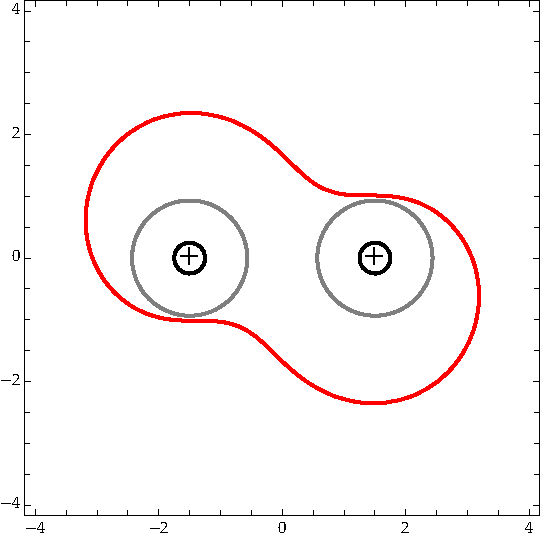
\includegraphics[width=\linewidth]{img/penrose_binaries/sks_regions.pdf}
  \caption{Regions of interest in the $t=0$ \ac{SKS} metric. The red region marks the boundary of the local ergosphere while the gray and black regions mark, respectively, the event horizons and singularities. The black crosshairs mark the centers of the black holes. The spacetimes parameters were chosen to be $M^{(1)} = M^{(2)} = 1/2$, $a^{(1)} = a^{(2)} = 1/4$ and $b = 3$}
  \label{fig:sks_ergo_plot}
\end{figure}

\subsubsection{Example 1}
\label{ch:sks_example_1}

For our first example, we have chosen the system parameters as $M^{(1)} = M^{(2)} = 1/2$, $a^{(1)} = a^{(2)} = 0.49$ and $b = 10$. The break-up point was chosen at coordinates $X^i = (6.3, 0, 0)$ and the background sphere radius was chosen to be $1.0 \times 10^6$. Following the same template of Table~\ref{tab:arbitrary_penrose_kerr_example_energy_mass}, Table~\ref{tab:arbitrary_penrose_sks_example_energy_mass} summarizes the initial energy and mass of the participating particles.

Once again, the first, second and third rows contain data relative to the entry, Penrose and exit orbits, respectively. The parameters for the entry and Penrose orbits are chosen explicitly, while the parameters of the exit orbit are computed via the conservation of 4-momentum at the break-point. The masses are explicitly chosen in order to satisfy Eq.~\eqref{eq:mass_constraint} and to provide a way of computing initial velocities via Eqs.~\eqref{eq:arbitrary_penrose_ellipse_parametric_1}-\eqref{eq:arbitrary_penrose_ellipse_parametric_2}
%
\begin{table}[]
  \centering
  \begin{tabular}{cc}
    \hline\hline
    $E(0)$                              & $m$                                 \\
    $1.0$                               & $1.0 \times 10^{-1}$                \\
    $8.0 \times 10^{-3}$                & $1.0 \times 10^{-4}$                \\
    $9.9199999999999999 \times 10^{-1}$ & $9.5800493929022838 \times 10^{-3}$ \\ \hline\hline
  \end{tabular}
  \caption{Initial energy and masses for the particles participating in the \ac{PP} example in the \ac{SKS} background.}
  \label{tab:arbitrary_penrose_sks_example_energy_mass}
\end{table}

Once more, following Table~\ref{tab:arbitrary_penrose_kerr_example_velocities}, Table~\ref{tab:arbitrary_penrose_sks_example_velocities} summarizes the initial velocities of the participating particles. Here, the values of the first two rows (representing the ingoing and Penrose trajectories, respectively), were computed via the parametrization described in the previous section together with data from Tab.~\ref{tab:arbitrary_penrose_kerr_example_energy_mass} while data on the third row, representing the outgoing particle, was computed via conservation of 4-momentum. The third column in this table shows the value of the ellipse parameter chosen for each orbit (except the exit orbit).
%
\begin{table}[]
  \centering
  \begin{tabular}{ccc}
    \hline\hline
    $V^x(0)$              & $V^y(0)$              & $\Theta$       \\
    $0.6769503786998466$  & $0.6740022058848380$  & $-25/200 \pi$  \\
    $0.5948571400034293$  & $-0.3343724878526367$ & $-100/200 \pi$ \\
    $0.66011565390809868$ & $0.68380243736284951$ & ---            \\ \hline\hline
  \end{tabular}
  \caption{Initial velocities for the particles participating in the \ac{PP} example in the \ac{SKS} background.}
  \label{tab:arbitrary_penrose_sks_example_velocities}
\end{table}

As Table~\ref{tab:arbitrary_penrose_kerr_example_results}, Table~\ref{tab:arbitrary_penrose_sks_example_results} summarizes the two energy measures (local and global on the first and second column, respectively) at the time when they hit the background sphere. The first row contains data relative to the ingoing orbit while the second contains data relative to the outgoing orbit. Note that $t_f$ does not necessarily coincide for the two orbits, since they might take arbitrarily long paths before escaping to infinity. The third column shows the absolute difference between global and local energies at the background sphere.
%
\begin{table}[]
  \centering
  \resizebox{\textwidth}{!}{
    \begin{tabular}{ccc}
      \hline\hline
      $E(t_f)$                            & $\varepsilon(t_f)$                  & $|E(t_f) - \varepsilon(t_f)|$       \\
      $2.4452985315377770 \times 10^{-1}$ & $2.4453006741751246 \times 10^{-1}$ & $2.1426373481014949 \times 10^{-7}$ \\
      $3.4638508542318119 \times 10^{-1}$ & $3.4638400572434974 \times 10^{-1}$ & $1.0796988314520917 \times 10^{-6}$ \\ \hline\hline
    \end{tabular}
  }
  \caption{Energy measures at the time of collision with the background sphere in the \ac{SKS} background}
  \label{tab:arbitrary_penrose_sks_example_results}
\end{table}

Finally, following Table~\ref{tab:arbitrary_penrose_kerr_example_efficiency}, Table~\ref{tab:arbitrary_penrose_sks_example_efficiency} summarizes the amount of energy extracted from the process in different forms. The first and second rows compute the difference between the energy of the outgoing and ingoing particles using different energy measures (local and global respectively). Since this difference is positive, we can conclude that energy was indeed extracted from the black hole. The last two rows compute the efficiency of the process for the two available energy measures, given by Eq~\eqref{eq:arbitrary_penrose_kerr_example_efficiency_formula}.
\begin{table}[]
  \centering
  \begin{tabular}{cc}
    \hline\hline
    $E_\text{out}(t_f)-E_\text{in}(t_f)$                     & $0.10185523226940352$ \\
    $\varepsilon_\text{out}(t_f)-\varepsilon_\text{in}(t_f)$ & $0.10185393830683726$ \\
    $\eta_E$                                                 & $0.41653495863897544$ \\
    $\eta_\varepsilon$                                       & $0.41652966700464295$ \\ \hline\hline
  \end{tabular}
  \caption{Energy difference and extraction efficiency of the process given different energy measures in the \ac{SKS} background.}
  \label{tab:arbitrary_penrose_sks_example_efficiency}
\end{table}

\subsubsection{Example 2}
\label{ch:sks_example_2}

In this example, we repeat the run detailed in Sec.~\ref{ch:sks_example_1} while changing the distance parameter from $b=10.0$ to $b = 7.21$. We have also changed the break-up point coordinates in each run so that it remains at $1.3$ coordinate distance units to the right of the right-most black hole. The results of this variation are summarized in Table~\ref{tab:arbitrary_penrose_sks_example_results_d_variation} where it is possible to see that the efficiency decreases as the black wholes get more distant from each other.

\begin{table}[]
  \centering
  \begin{tabular}{ccc}
    \hline\hline
    $d$  & $\eta_E$             & $\eta_\varepsilon$   \\
    10.0 & $0.4165349586389754$ & $0.4165293020302941$ \\
    9.69 & $0.4099912589653710$ & $0.4099855399919209$ \\
    9.38 & $0.4042822480170929$ & $0.4042767439403118$ \\
    9.07 & $0.3994849072973370$ & $0.3994792027270561$ \\
    8.76 & $0.3954568832639254$ & $0.3954513766173146$ \\
    8.45 & $0.3915618006432178$ & $0.3915564144708418$ \\
    8.14 & $0.3857189791093659$ & $0.3857135001267253$ \\
    7.83 & $0.3709406424619314$ & $0.3709350873643125$ \\
    7.52 & $0.3205512719659607$ & $0.3205458837844264$ \\
    7.21 & $0.1207168410527975$ & $0.1207122709189437$ \\ \hline\hline
  \end{tabular}
  \caption{Energy extraction efficiency for the configuration detailed in Sec~\ref{ch:sks_example_1} while varying the distance parameter $b$ and keeping the break-up point at $1.3$ coordinate distance unites to the right of the rightmost black hole in the \ac{SKS} background.}
  \label{tab:arbitrary_penrose_sks_example_results_d_variation}
\end{table}

\subsubsection{Example 3}
\label{ch:sks_example_3}

In this example we vary the mass of the left-most black hole $M^{(2)}$ from $0.5$ to $0.275$ while also changing the spin parameter according to $a^{(2)} = 0.98 M^{(2)}$. We keep fixed the mass $M^{(1)} = 0.5$, the spin parameter $a^{(1)} = 0.49$, the distance parameter $b=20.0$ and the break-up point $(11.0, 0.0, 0.0)$. This configuration is analogue to that of the single Kerr black hole example of Sec.~\ref{ch:kerr_example}. The results are summarized in Table~\ref{tab:arbitrary_penrose_sks_example_results_M2_variation}, where it is possible to see that as the mass of the companion black hole decreases, the extraction efficiency decreases.

\begin{table}[]
  \centering
  \begin{tabular}{ccc}
    \hline\hline
    $M2$  & $\eta_E$             & $\eta_\varepsilon$   \\
    0.500 & $0.1057279994029897$ & $0.1057236710602922$ \\
    0.475 & $0.0870377969920106$ & $0.0870336429442202$ \\
    0.450 & $0.0712047949044382$ & $0.0712008663973118$ \\
    0.425 & $0.0578255784926676$ & $0.0578218053066227$ \\
    0.400 & $0.0465203386664686$ & $0.0465166569217887$ \\
    0.375 & $0.0369572283763885$ & $0.0369537431441037$ \\
    0.350 & $0.0288551456052595$ & $0.0288518045002344$ \\
    0.325 & $0.0219792546154663$ & $0.0219759777138235$ \\
    0.300 & $0.0161341223097530$ & $0.0161310745614111$ \\
    0.275 & $0.0111575173287062$ & $0.0111545996429916$ \\ \hline\hline
  \end{tabular}
  \caption{Energy extraction efficiency for fixed mass $M^{(1)} = 0.5$, spin parameter $a^{(1)} = 0.49$, distance parameter $b=20.0$ and break-up point $(11.0, 0.0, 0.0)$ and varying Mass $M^{(2)}$ and spin parameter $a^{(2)} = 0.98 M^{(2)}$.}
  \label{tab:arbitrary_penrose_sks_example_results_M2_variation}
\end{table}


\myclearpage
\par

\chapter{Numerical Scalar Wave Scattering in GW150914}
\label{ch:wave_scattering}
\section{Chapter Introduction}
\label{ch:wave_scattering:sec:intro}
In this chapter, we will focus on the numerical simulation of a scalar wave scattering off a black hole binary that mirrors the first event detected by LIGO, know as GW150914. Due to the challenges imposed by the strong gravity regime and the highly dynamic nature of astrophysical binary systems already discussed in Chapter \ref{ch:introduction}, to accurately simulate wave scattering around black hole binaries, it is necessary to solve Einstein's field equations numerically. In recent years, significant progress has been made in the numerical simulation of black hole binaries thanks to state-of-the-art strongly hyperbolic reformulations of the field equations, such as the BSSN formulation~\cite{PhysRevD.52.5428,PhysRevD.59.024007} and advancements in the understanding of stability criteria in partial differential equation discretization schemes employing techniques such as summation by parts~\cite{Diener2007}. These techniques have enabled us to simulate the dynamics of black hole binaries and their gravitational wave emission with unprecedented accuracy, stability and reliability.

Numerical evolution through self-coding can be a daunting task. This is where the employment of pre-existing tools, such as the \texttt{EinsteinToolkit}~\cite{EinsteinToolkit:2022_11}, becomes beneficial. The \texttt{EinsteinToolkit} is, according to its home page, ``a community-driven software platform of core computational tools to advance and support research in relativistic astrophysics and gravitational physics.''. The \texttt{EinsteinToolkit} is composed of a variety of software modules, referred to as \texttt{Thorns}, that are integrated into the \texttt{Cactus}~\cite{Cactuscode:web,Cactusprize:web,Goodale:2002a} computational framework. Each \texttt{Thorn} has the ability to perform a range of tasks, including infrastructure tasks such as file input/output, adaptive mesh refinement (AMR), as well as physics-related tasks such as the evolution of binary systems, the extraction of gravitational waves, and the multipole decomposition of a signal.

In the following sections, I will introduce the equations utilized for the evolution of a scalar wave atop a numerically metric without back-reaction, where the spacetime evolution disregards the scalar field's contribution to its stress-energy-momentum tensor. Subsequently, I will provide a detailed description of the \texttt{EinsteinToolkit Thorn KleinGordon} responsible for this evolution, and present the results that have been obtained thus far. The scalar field evolution code was developed by the author and its available, together with useful resources, in the \texttt{GitHub} repository~\cite{FieldPerturbationsRepo}. It is hoped that these results will offer valuable insights into the dynamics of the relaxation of astrophysical binary systems when perturbed.

\section{Mathematical formulation}
\label{ch:wave_scattering:sec:math}
\subsection{Evolution System}

The formulation employed in this chapter was initially developed and published in Ref.~\cite{PhysRevD.96.104040}. Although the primary focus of that publication differs from the subject matter of this chapter, Appendix A of the paper contains the 3+1 decomposed Klein-Gordon equation for a massive scalar field, as presented in equations A3c and A3d. For the sake of completeness, these equations are
%
\begin{align}
  \partial_t \Phi =   & -2 \alpha K_\phi + \mathcal{L}_\beta \Phi \label{eq:wave_scattering_a3c}                                                                                                                                                     \\
  \partial_t K_\Phi = & \alpha \left( K K_\Phi - \frac{1}{2} \gamma^{ij} D_i \partial_j \Phi + \frac{1}{2} \mu^2 \Phi \right) - \frac{1}{2} \gamma^{ij} \partial_i \alpha \partial_j \Phi + \mathcal{L}_\beta K_\Phi, \label{eq:wave_scattering_a3d}
\end{align}
%
where $\Phi$ is the scalar field being evolved, $K_\Phi$ its ``canonical momentum'', given by
%
\begin{equation}
  K_\Phi = -\frac{1}{2\alpha} \left( \partial_t - \mathcal{L}_\beta \right)\Phi,
  \label{eq:wave_scattering_a2}
\end{equation}
%
$\alpha$ is the spacetime lapse, $\beta^i$ its shift vector, $\gamma^{ij}$ its induced 3-metric, $K$ the trace of its extrinsic curvature tensor, $D_i$ the covariant derivative associated with $\gamma^{ij}$, $\mu$ the spacetime mass parameter and $\mathcal{L}_\beta$ is the Lie derivative along the shift vector $\beta^i$, given explicitly by
%
\begin{equation}
  \mathcal{L}_\beta\Phi = \beta^i \partial_i \Phi.
  \label{eq:wave_scattering_lie_derivative}
\end{equation}

To expand each component of these equations, we utilized the mathematical software package \texttt{Wolfram Mathematica}. The resulting expansion was subsequently implemented into the \texttt{Thorn} by automatically generating corresponding \texttt{C} code from within \texttt{Mathematica}. The code used in this process can be found in \texttt{Notebooks/equations.nb} of the \texttt{Thorn}'s repository.

\subsection{Initial data}

The implementation supports three distinct initial conditions for the scalar field and its canonical momentum. These include a plane wave, an exact Gaussian, and a multipolar Gaussian function. The plane wave and exact Gaussian initial data were developed for the purpose of testing multipatch derivatives in flat spacetime, which will be elaborated on further in subsequent sections. The exact Gaussian initial data is named as such to reflect the fact that it is an exact solution of the Klein-Gordon equation in flat spacetime.

The multipolar Gaussian function is a basic Gaussian function that is multiplied by a linear combination of real spherical harmonics. This particular function was the one chosen during our ``production'' runs as it has the ability to excite specific modes in the system based on the chosen parameters for the linear combination. The development of this initial data is based on the methodology presented in Ref.~\cite{PhysRevD.87.043513}. In order to construct it, let us first introduce its components. We start with the Gaussian function $G(r, \sigma)$, given by
%
\begin{equation}
  G(r, \sigma) = \exp\left( -\frac{1}{2} \left( \frac{r}{\sigma} \right)^2  \right).
  \label{eq:wave_scattering_gaussian}
\end{equation}
%
where $\sigma$ is the Gaussian width parameter. Next, we introduce the real spherical harmonics $Y_{lm}(x,y,z)$, given by
%
\begin{equation}
  Y_{lm}(x, y, z) =
  \begin{cases}
    A_{lm} P_{lm}\left( \frac{z}{\sqrt{x^2 + y^2 + z^2}} \right) \cos(m \arctan(y,x)) \text{ if } m \geq 0  \\
    A_{lm} P_{l|m|}\left( \frac{z}{\sqrt{x^2 + y^2 + z^2}} \right) \sin(|m| \arctan(y,x)) \text{ if } m < 0 \\
  \end{cases}
  ,
  \label{eq:wave_scattering_real_spherical_harmonics}
\end{equation}
%
where $P_{lm}(x)$ are the associated Legendre polynomials and the $A_{lm}$ coefficients are given by
%
\begin{equation}
  A_{lm} = (-1)^m \sqrt{\frac{2 l + 1}{4\pi} \frac{(l-m)!}{(l+m)!}}.
  \label{eq:wave_scattering_real_spherical_harmonics_coeffs}
\end{equation}
%
By introducing ``shifted coordinates''
%
\begin{align}
  X & \equiv x - x_0 \label{eq:wave_scattering_real_spherical_harmonics_shifted_x}                \\
  Y & \equiv y - y_0 \label{eq:wave_scattering_real_spherical_harmonics_shifted_y}                \\
  Z & \equiv z - z_0 \label{eq:wave_scattering_real_spherical_harmonics_shifted_z}                \\
  R & \equiv \sqrt{X^2 + Y^2 + Z^2} \label{eq:wave_scattering_real_spherical_harmonics_shifted_r} \\
\end{align}
%
it is possible to shift the location of the center of the function to $(x_0,y_0,z_0)$. Combining these pieces, the multipolar Gaussian function $M_G(x,y,z)$ is written as
%
\begin{equation}
  M_G(x, y, z) = \sum_{l=0}^{N}\sum_{m = -l}^{l} c_{l m} Y_{l m}(X,Y,Z) G(R-R_0,\sigma)
  \label{eq:wave_scattering_multipolar_gaussian}
\end{equation}
%
where $R_0$ is the radius of the Gaussian function. Once again, code generation routines for the initial data can be found in \texttt{Notebooks/equation.nb}. It is important to note that in the implemented code, the series is expanded up to $N = 2$, and higher multipole orders are not supported.

Figure~\ref{fig:multipolar_gaussian_id_demo} showcases three distinct configurations of the multipolar Gaussian function. For all panels, the parameters $x_0$, $y_0$, and $z_0$ were assigned a value of zero, while $R_0$ was set to 5. Panel \textbf{A} displays a plot where $c_{00}$ is assigned a value of $1/A_{00}$, and all other coefficients are set to zero. In Panel \textbf{B}, $c_{11}$ is set to $1/A_{11}$, and all other coefficients are set to zero. Finally, in Panel \textbf{C}, $c_{22}$ is assigned a value of $1/(3A_{22})$, and all other coefficients are set to zero.

\begin{figure}[!ht]
  \centering
  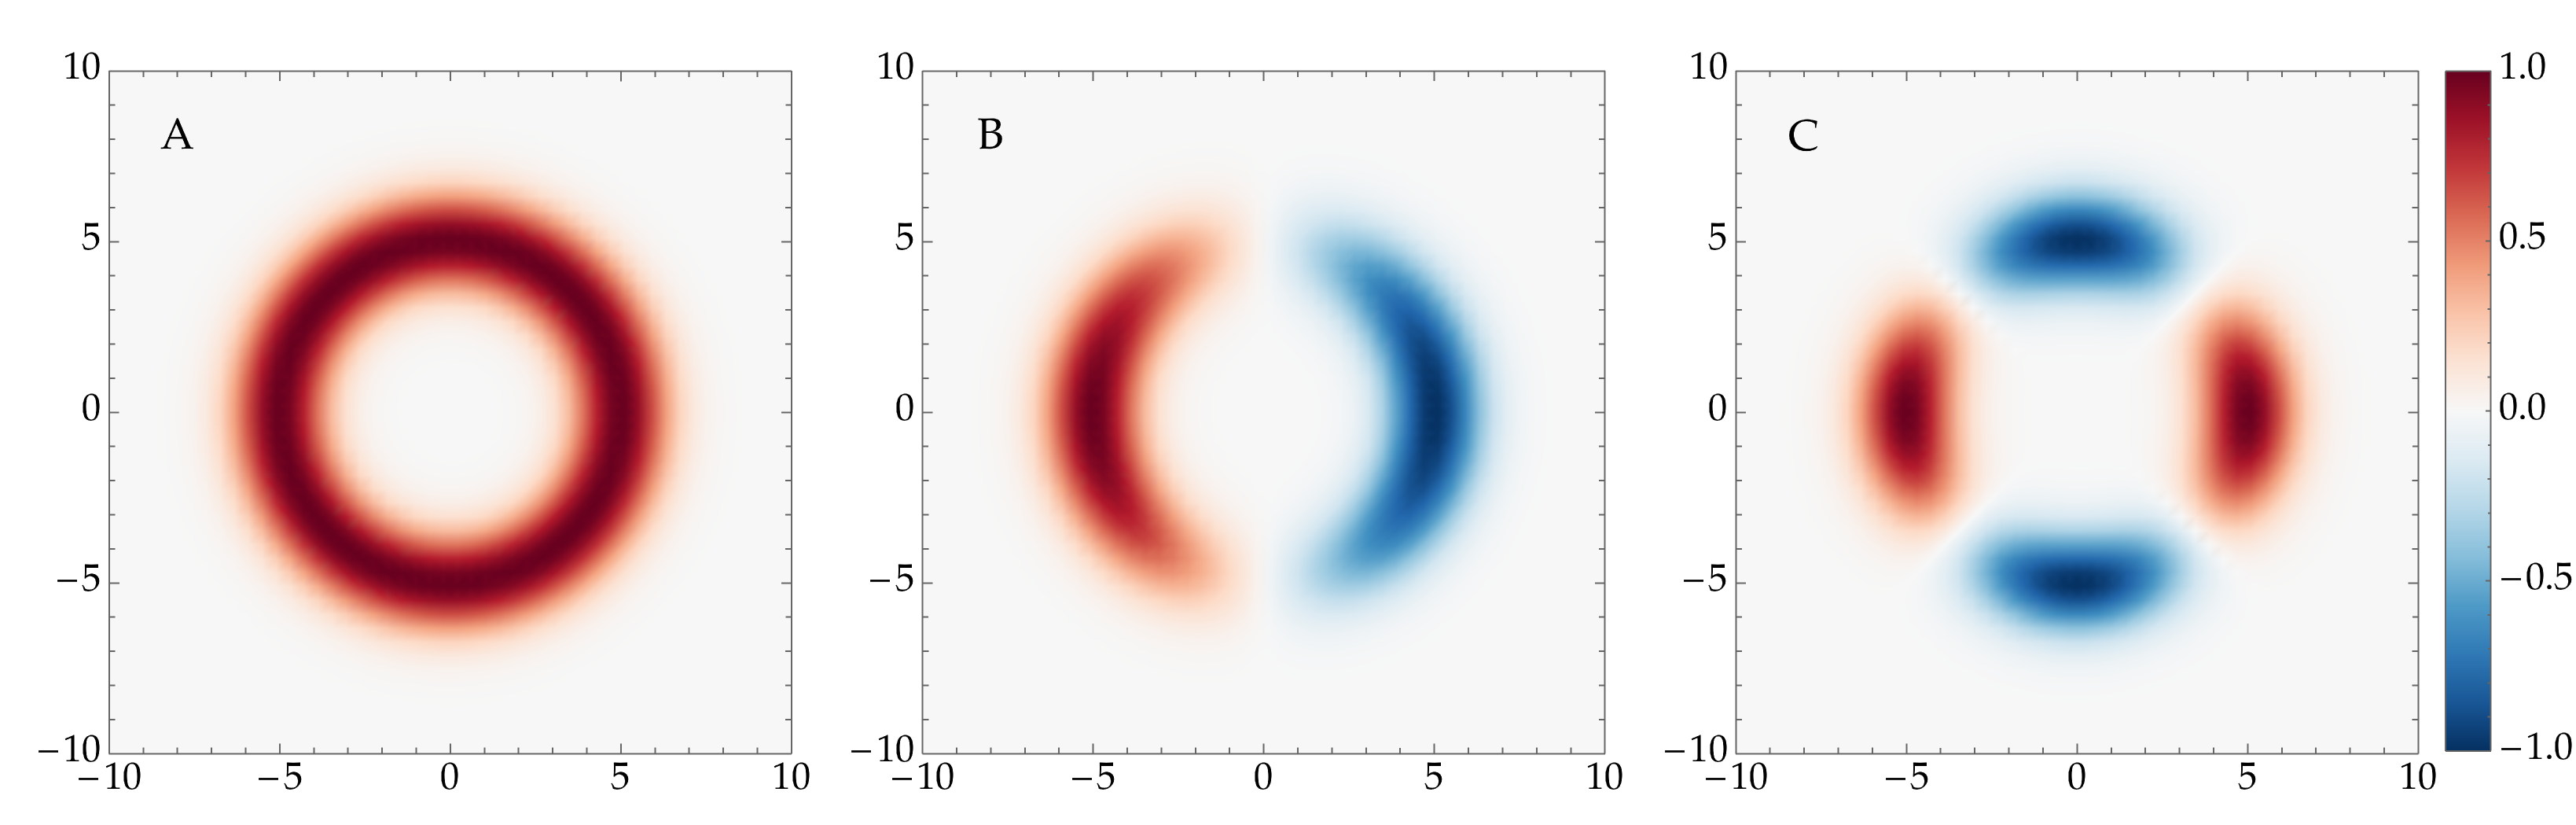
\includegraphics[width=\linewidth]{img/wave_scattering/multipolar_gaussian_id_examples.png}
  \caption{Demonstration of the multipolar Gaussian function with different parameters. For all panels, $x_0 = y_0 = z_0 = 0$ and $R_0 = 5$. In Panel \textbf{A} displays the only nonzero coefficient is $c_{00} = 1/A_{00}$, in Panel \textbf{B}, $c_{11} = 1/A_{11}$, and in Panel \textbf{C}, $c_{22} = 1/(3A_{22})$.}
  \label{fig:multipolar_gaussian_id_demo}
\end{figure}

\subsection{Evolution Code}

The coordinate system used in our grid setup was the \texttt{Thornburg04} coordinates, implemented through the \texttt{Llama}~\cite{PhysRevD.83.044045} infrastructure. This coordinate system comprises spherical wedges, each covering 90 degrees in all three dimensions, and centered on the $+x$, $-x$, $+y$, $-y$, $+z$, and $-z$ axes. These wedges provide complete coverage of a region between $r_\text{min}$ and $r_\text{max}$, with smooth inner and outer boundaries, and a cubical patch enclosing $r < r_\text{min}$ where standard \texttt{Carpet}~\cite{Schnetter:2003rb} box-in-box mesh refinement can be applied.

To set up the gravitational initial data, we used \texttt{TwoPunctures}~\cite{Ansorg:2004ds} with parameters that emulate the GW150914 merger. Gravitational evolution was performed using \texttt{ML\_BSSN}~\cite{Brown:2008sb,Kranc:web,McLachlan:web} with a $1+\log$ slicing condition and a $\Gamma$-driver shift. We employed 7 levels of mesh refinement boxes via \texttt{Carpet}, centered around each of the punctures and tracking their motion via \texttt{PunctureTracker}. We developed the \texttt{KleinGordon Thorn}, which we describe in this section, to evolve a massless scalar field with initial data provided by a multipolar Gaussian function, centered around the origin with $R_0 = 15.0$, width $\sigma = 1.0$, and the only non-zero multipolar coefficient being $c_{00} = 1 / A_{00}$. This spherically symmetric initial data allowed us to activate reflection symmetry around the $+z$ plane in the code, which saved computational time, memory, and storage space.

In the gravitational evolution code, spatial derivatives were provided by \texttt{SummationByParts}~\cite{Diener:2005tn}, which provides finite difference stencils satisfying the summation-by-parts property with embedded Kreiss-Oliger type artificial dissipation. In \texttt{KleinGordon}, we utilized handcrafted central finite difference stencils and added artificial Kreiss-Oliger dissipation to the evolved Klein-Gordon fields via \texttt{Dissipation}. The gravitational evolution code projected its derivative operators into the global coordinate system utilized by \texttt{Llama} via \texttt{GlobalDerivative}, but in \texttt{KleinGordon}, this projection was also handcrafted via the Jacobian and Jacobian derivative components provided by \texttt{Llama}. Code generation for these projections can be found in the \texttt{Notebooks/equations.nb} notebook. Both evolutions utilized 8th order finite difference stencils, and radiating boundary conditions were employed in the outer boundaries via \texttt{NewRad}.

The time integration method utilized in this study was \texttt{MoL}. A 4th order Runge-Kutta method with fixed time step was employed for the time integration process. It is important to note that \texttt{Carpet} employs different time steps for various refinement levels, thus the time step specified in the parameter files pertains to the coarsest level. The final integration time was selected in conjunction with the outer boundary radius to minimize interference from reflections at the outer boundaries, inter-patch boundaries, and inter-refinement level boundaries on the scalar field signal being measured.

At regular time intervals, data was extracted at $7$ different radii using \texttt{Multipole}, as well as 2D and 3D field data evolved by \texttt{KleinGordon}. Additionally, statistics such as puncture locations were recorded, which enabled the construction of visualizations of the simulated data. These results will be presented shortly. The parameter file used for this evolution can be located in the specified GitHub repository under \texttt{KleinGordon/par/GW150914/GW150914\_Scalar\_field.par}.

\subsection{Results}

\begin{figure}
  \centering
  \animategraphics[autoplay, loop, width=\linewidth]{12}{img/wave_scattering/movie/Phi_xy_00}{00}{75}
  \caption{Example .gif animation}
\end{figure}

%0 7 19 29

\myclearpage
\par

\chapter{Quasinormal Modes and the Asymptotic Iteration Method}
\label{ch:qnm_aim}
When a closed physical system (like a guitar string) is perturbed, it relaxes by emitting certain natural frequencies know as \emph{normal modes}. If, however, the system is open (and therefore energy is being somehow dissipated away), its emitted natural frequencies will decay with time (like for instance sounding a bell in a church). These decaying modes are called \emph{quasinormal modes} (QNMs). Such frequencies can be used to obtain information about the system that produces them and black holes, like church bells, are also subject to these phenomena: Perturbed black holes relax by emitting waves in characteristic frequencies that decay with time, thanks to the dissipative nature of the event horizon. See Refs.~\cite{review1, review2, review3, review4} for an in-depth review of the quasinormal mode problem in the context of general relativity and black holes. Determining these characteristic frequencies quickly and accurately for a large range of models is important for many practical reasons. It has been shown that the gravitational wave signal emitted at the final stage of the coalescence of two compact objects is well described by quasinormal modes~\cite{buonanno,seidel}. This means that if one has access to a database of quasinormal modes and of gravitational wave signals from astrophysical collision events, it is possible to characterize the remnant object using its quasinormal frequencies. Since there are many models that aim to describe remnants, being able to compute the quasinormal frequencies for such models reliably is paramount for confirming or discarding them. Very often, computing quasinormal modes reduces to finding the discrete eigenvalue set of a second order differential equation with appropriate boundary conditions and asymptotic behavior. In this chapter, we will explore a numerical technique recently developed for tackling this problem, known as the \emph{Asymptotic Iteration Method} (AIM). The groundwork of the technique was laid out in Ref.~\cite{aim_original} and in Ref.~\cite{aim_improved} the method was refined and adapted to GR.

Motivated by these developments, we have implemented \texttt{QuasinormalModes.jl} (see the acompanying paper in Ref.~\cite{Sanches2022}), a \texttt{Julia}~\cite{Bezanson2017} software package for finding quasinormal modes using the AIM. Not only that, the package can be used to compute the discrete eigenvalues of \emph{any} second order homogeneous ODE (such as the energy eigenstates of the time independent Schrödinger equation) provided that these eigenvalues actually exist. The package features a flexible and user-friendly API where the user simply needs to provide the coefficients of the problem ODE after incorporating boundary and asymptotic conditions on it. The user can also choose to use machine or arbitrary precision arithmetic for the underlying floating point operations involved and whether to do computations sequentially or in parallel using threads. The API also tries not to force any particular workflow on the users so that they can incorporate and adapt the existing functionality on their research pipelines without unwanted intrusions. Often user-friendliness, flexibility and performance are treated as mutually exclusive, particularly in scientific applications. By using \texttt{Julia} as an implementation language, the package can have all these features simultaneously. Another important motivation for using \texttt{Julia} and writing this package was the lack of generalist, free (both in the financial and license-wise sense) open source tools that serve the same purpose. More precisely, there are tools which are free and open source, but run on top of a proprietary paid and expensive software framework such as the ones developed in Refs.~\cite{qnmspectral,spectralbp}, which are both excellent packages that aim to perform the same task as \texttt{QuasinormalModes.jl} and can be obtained and modified freely but, unfortunately, require the user to own a license of the proprietary \texttt{Wolfram Mathematica} CAS. Furthermore, their implementations are limited to solve problems where the eigenvalues must appear in the ODE as polynomials of order $p$. While this is not prohibitively restrictive to most astrophysics problems, it can be an important limitation in other areas. There are also packages that are free and run on top of \texttt{Mathematica} but are not aimed at being general eigenvalue solvers at all, such as the one in Ref.~\cite{bhpt_quasinormalmodes}, that can only compute modes of Schwarzschild and Kerr black holes. Finally, the \texttt{Python} package in Ref.~\cite{bhpt_qnm} is open source and free but can only compute Kerr quasinormal modes. \texttt{QuasinormalModes.jl} fills the existing gap for free, open source tools that are able to compute discrete eigenvalues (and in particular, quasinormal modes) efficiently for a broad class of models and problems. The package was used in Ref.~\cite{Mamani2022} where non-scalar perturbations were considered. Novel frequencies were obtained and results were compared against literature values, when possible, while also cross-checking results for the same models obtained via the more traditional pseudo-spectral method.


\section{Perturbation equations}
\label{ch:qnm_aim:sec:equations}
The spacetime metric for a spherically symmetric Schwarzschild black hole, is given by \cite{Schwarzschild:1916uq}
%
\begin{equation}\label{eq:Metric}
  ds^2=-f(r)\,dt^2+\frac{1}{f(r)}dr^2+r^2d\theta^2+
  r^2\sin^2{\theta}\,d\varphi^2,
\end{equation}
%
where the horizon function is given by
%
\begin{equation}\label{EqHoriFuncHayward}
  f(r)=1-\frac{2M}{r},
\end{equation}
%
where $M$ is the mass of the black hole, and $r$ is the radial coordinate which, in principle, belongs to the interval $r\in [0,\, \infty)$.

The coordinates employed in the metric described by Eq.~\eqref{eq:Metric} are commonly known as Schwarzschild coordinates. This metric features an event horizon located at $r=2M$ and a physical singularity at $r=0$. In the asymptotic region, namely as $r$ approaches infinity, the metric reduces to a flat metric. For the purposes of examining quasinormal modes in this black hole spacetime, the relevant region of the spacetime is the range of the radial coordinate $r$ between $2M$ and infinity.

Our analysis of linear perturbations in the Schwarzschild black hole spacetime described by \eqref{eq:Metric} follows the standard procedure. After selecting a specific perturbation field, we reduce the corresponding partial differential equations to a unique Schrödinger-like ordinary differential equation using a series of transformations. In this approach, the perturbation functions were decomposed into Fourier modes of the form $e^{i\omega t}=e^{i(\omega_{Re}-i \omega_{Im})t}=e^{\omega_{Im} t}\cos{\left(\omega_{Re} t\right)}$. This eliminated the time derivatives from the differential equations, while the angular dependence was handled through expansion in spherical harmonics.

It is important to be reminded at this point that ordinary \acp{QNM} are characterized by frequencies with both non-zero real and imaginary components and represent oscillatory solutions that are exponentially suppressed by the imaginary component of the frequency. In contrast, modes with purely imaginary frequencies, where the real part of the frequency is zero, correspond to purely damping solutions since the respective perturbation functions decay as $ e^{i\omega t}=e^{\omega_{Im} t}$.

\subsection{Spin $0$, $1$ and $2$ perturbations}

The computation of perturbations of integer spin, including scalar, vector, and gravitational perturbations in the Schwarzschild black hole spacetime, is a well understood and solved problem with a significant body of literature dedicated to it. This literature is of great interest for our purposes, which involve comparisons and calibrations. In fact, it has been shown that the equations of motion can be expressed in a concise form known as Schrödinger-like differential equations (see, for instance, \cite{review3}). Thus, for massless scalar ($s=0$), electromagnetic ($s=1$), and vector-type gravitational perturbations ($s=2$), the Schrödinger-like equations take the following form:
%
\begin{equation}\label{Eq:IntegerSpin}
  \frac{d^2 \psi_{{s}}(r)}{d r_*^2}
  +\left[\omega^2-V_{{s}}(r)\right]\psi_{{s}}(r)=0,
\end{equation}
%
where the potential function $V_{s}(r)$ is given by
%
\begin{equation}\label{Eq:IntegerSpinPot}
  V_{s}(r)=f(r)\left[\frac{\ell\left(\ell+1\right)}{r^2}
    +\left(1-s^2\right)\frac{2M}{r^3}\right],
\end{equation}
%
and the tortoise coordinate $r_*$ is defined in terms of the areal coordinate $r$ by $dr_*=dr/f(r)$. The problem of calculating quasinormal frequencies is therefore reduced to an eigenvalue problem, which can be solved by either expanding the function $\psi$ in a base composed of special functions or solving the second-order differential equation directly once appropriate asymptotic boundary conditions have been specified.

It is important to note that the potential function in Eq.~\eqref{Eq:IntegerSpinPot} is zero at the horizon because $f(r_h)=0$. Thus, the Schr\"odinger-like equation reduces to a single harmonic oscillator problem, whose solutions are given by
%
\begin{equation}
  \psi_{s}(r)=c_1\, e^{-i\omega r_*}+c_2\, e^{i\omega r_*}, \quad r\to r_h.
  \label{eq:sol1}
\end{equation}
%
The first term in Eq.~\eqref{eq:sol1} is interpreted as an ingoing wave, i.e., a wave that travels inward and eventually falls into the black hole event horizon. The second term is interpreted as an outgoing wave, i.e., a wave that travels outward with respect to the black hole and can escape to spatial infinity. Considering that perturbation theory is implemented using classical assumptions, nothing is expected to come out from the black hole interior, thus, in the following analysis we impose ingoing solutions as boundary conditions at the horizon and discarding outgoing solutions altogether. This is accomplished by setting  $c_2=0$.

At spatial infinity, however, one has $f(r)\to 1$ and the effective potential of Eq.~\eqref{Eq:IntegerSpinPot} also vanishes. Thus, in such a limit the general solutions to the wave equation \eqref{Eq:IntegerSpin} have the same form as the function given in Eq.~\ref{eq:sol1}, i.e.,
%
\begin{equation}
  \psi_{s}(r_*)=c_3\, e^{-i\omega r_*}+c_4\, e^{i\omega r_*}, \quad r\to \infty.
\end{equation}
%
The first solution can be interpreted as waves that originate sufficiently far away from the black hole and can be avoided by setting $c_3=0$. Conversely, the second solution can be interpreted as waves that leave the universe, serving as the boundary condition at spatial infinity. It is important to note that neither the angular momentum $\ell$ nor the perturbing field's spin have an explicit influence on the boundary conditions.

It is interesting to note that close to the event horizon, the tortoise coordinate becomes
%
\begin{equation}
  r_*=\int \frac{dr}{f'(r_h)(r-r_h)}\approx \frac{\ln{(r-r_h)}}{ f'(r_h)},\quad r\to r_h
\end{equation}
where $r_h=2M$.
Thus, when written in terms of the radial coordinate, the boundary condition at the horizon becomes ($f'(r_h)=1/r_h$)
%
\begin{equation}
  \psi_s(r)\sim e^{-i\omega \frac{\ln{(r-r_h)}}{f'(r_h)}}\sim \left(r-r_h\right)^{-i\frac{\omega}{f'(r_h)}}.
\end{equation}
%
In turn, the tortoise coordinate at the spatial infinity becomes
%
\begin{equation}
  r_*=\int \frac{dr}{f(r)}\approx r+r_h\,\ln{r},\quad r\to \infty
\end{equation}
%
while the asymptotic solution at spatial infinity becomes
%
\begin{equation}
  \psi_s(r)\sim e^{i\omega(r+ r_h \ln{r})}\sim r^{i\, r_h\omega}e^{i\omega r}.
\end{equation}

We shall now work in terms of new coordinates defined by $u\equiv2M/r$. This is equivalent to choosing $u=1/r$ and then normalizing the mass $M$ to $2M=1$. The relation between the tortoise coordinate $r_*$ and the new coordinate $u$  becomes $du/dr_*=-u^2f(u)$. We shall also constrain our analysis to the outer region of the black hole, such that $r_h\leq r<\infty$. Hence, in terms of the new coordinate, this region is bounded to the interval $u\in [0,\, 1]$, and the potential becomes
%
\begin{equation}
  V_{s}(u)=f(u)\,u^2\left[\ell\left(1+\ell\right)+\left(1-s^2\right)\,u\right],
\end{equation}
%
where $f(u) = 1- \,u$.

In numerical codes, it is frequently necessary to represent background quantities using horizon-penetrating Eddington-Finkelstein coordinates, as elaborated in Ref.~\cite{qnmspectral}. This is true despite the fact that we exclusively address perturbations outside the event horizon, as the coordinate singularity at the horizons can impede convergence and complicate the numerical solution of perturbation ODEs. We have developed a shortcut for writing the equations directly from the Schrödinger-like equation by implementing certain transformations. These transformations result in a differential equation that is equivalent to the one obtained from the Eddington-Finkelstein metric coordinates. In order to express the perturbation equations in terms of Eddington-Finkelstein coordinates, we utilize the transformation $\psi_{s}\to \Phi_s$, which is given by
%
\begin{equation}\label{Eq:TransN1}
  \psi_{s}= \frac{\Phi_{s}(u)}{u}e^{-i\omega\,r_*(u)}.
\end{equation}
%
Thus, Eq.~\eqref{Eq:IntegerSpin} becomes
%
%\begin{widetext}
\begin{equation}\label{Eq:IntegerSpin2}
  \begin{split}
    &\left[s^2u^2-\ell\left(\ell+1\right)u-2\,i\,\omega\right]\Phi_{s}(u)\\
    &-u\left(u^2-2\,i\,\omega\right)\Phi_{s}'(u)+\left(1-u\right)\,u^3\,\Phi_{s}''(u)=0,\end{split}
\end{equation}
%\end{widetext}
%
where we have set $M=1/2$ so that $r_h=1$. The asymptotic solutions close to the horizon may be calculated using the ansatz $\Phi_{s}(u)=(1-u)^{\alpha}$. By substituting this ansatz into Eq.~\eqref{Eq:IntegerSpin2} we get two solutions,
%
\begin{equation}\label{Eq:AsympHorion}
  \alpha=0,\qquad\qquad \alpha=2\,i\,\omega.
\end{equation}
%
The solution for $\alpha =0$ is interpreted physically as the ingoing waves at the horizon, while the other is interpreted as a wave coming out from the black hole interior, and thus, is neglected in the following analysis. In the same way, we consider the ansatz $\Phi_{s}=u^{\beta}$ to get the asymptotic solution close to the spatial infinity. Plugging this ansatz in Eq.~\eqref{Eq:IntegerSpin2} we get
%
\begin{equation}\label{Eq:AsymInfinite}
  \Phi_{s}(u)=c_5\,e^{2\,i\,\omega/u}u^{-2\,i\,\omega}+c_6\,u.
\end{equation}
%
We are interested in the divergent solution thus setting $c_6=0$. We then implement the final transformation, which takes into consideration the boundary conditions,
%
\begin{equation}\label{Eq:FinalTrans}
  \Phi_{s}(u)=e^{2\,i\,\omega/u}u^{-2\,i\,\omega}\phi_{s}(u),
\end{equation}
%
where $\phi_{s}(u)$ is a regular function in the interval $u\in[0,\,1]$ by definition. Finally, the equation of motion describing spin $0$, $1$, and $2$ perturbations is given by
%
\begin{equation}\label{Eq:IntegerSpin3}
  \begin{split}
    &\!\!\Big[\ell\left(\ell+1\right) u -s^2u^2-4\,i\lambda-16\,u\left(1+u\right)\lambda^2\Big]\phi_{s}(u)+\\
    & \!\!\Big[u^3+4i\,u\left(1-2u^2\right)\lambda\Big]\phi_{s}'(u)-(1-u)u^3\phi_{s}''(u)=0,
  \end{split}
\end{equation}
%
where we have used $\lambda=\omega M=\omega/2$. The final differential equation is then a quadratic eigenvalue problem in $\lambda$. It is also worth mentioning that in the limit of zero spin $s\to 0$, Eq.~\eqref{Eq:IntegerSpin3} reduces to Eq.~(4.8) of Ref.~\cite{qnmspectral}. These results just prove that the alternative way for getting the equations for the integer spin perturbations presented here is consistent with other approaches in the literature.

\subsection{Spin $1/2$ perturbations}

The differential equations for half-integer spin perturbations are quite distinct from Eq.~\eqref{Eq:IntegerSpin3}. See Ref.~\cite{Chandrasekhar1998-le} and references therein the mathematical foundations of black hole perturbation theory for higher spin fields. The equation for the spin $1/2$ Dirac field as a perturbation on the Schwarzschild background was derived in Ref.~\cite{Cho:2003qe} by using the Newman-Penrose formalism. The analysis was generalized for arbitrary half-integer spin in Ref.~\cite{Shu:2005fw}. The resulting equation of motion for the perturbations may be written in the Schr\"odinger-like form of Eq.~\eqref{Eq:IntegerSpin}, where the potential for the massless spin 1/2 field is given by
%
\begin{equation}\label{eq:pot-s12}
  V_{\scriptscriptstyle{1/2}}= \frac{\left(1+\ell\right)\sqrt{f(r)}}{r^{2}} \left[\left(1+\ell\right)\sqrt{f(r)}+\frac{3M}{r}-1\right].
\end{equation}

It is worth mentioning that we have found a typo in the definition of $\Delta$ in \cite{Cho:2003qe}, which must read $\Delta=r(r-2M)$.

We then implement the same transformations applied in the integer spin cases. First, we change the radial coordinate to $u=2M/r$, which is defined in the interval $u\in[0,1]$. Then by setting $2M=1$ the effective potential in Eq.~\eqref{eq:pot-s12} becomes
%
\begin{equation}
  \!\!V_{\scriptscriptstyle{1/2}}=\left(1+\ell\right)u^2\sqrt{f(u)} \left[\left(1+\ell\right)\sqrt{f(u)}+\frac{3u}{2} -1\right].
\end{equation}

It is interesting to point out that the asymptotic solutions do not depend on the spin of the field, and therefore the asymptotic solutions for this problem are the same as those obtained in Eqs.~\eqref{Eq:AsympHorion} and \eqref{Eq:AsymInfinite}. Similar transformations as those given in Eqs.~\eqref{Eq:TransN1} and~\eqref{Eq:FinalTrans} can then also be applied. Thus, the differential equation to be solved is given by
%
\begin{equation}\label{eq:onda-s12}
  \begin{split}
    &R(u)\phi_{\scriptscriptstyle{1/2}}(u) + Q(u)\phi_{\scriptscriptstyle{1/2}}'(u) + P(u) \,\phi_{\scriptscriptstyle{1/2}}''(u)=0,
  \end{split}
\end{equation}
%
in which the coefficients $R(u)$, $Q(u)$, and $P(u)$ are given by
%
\begin{eqnarray}
  R(u)=\,&& u^3+u(1+\ell)\left(1+\ell-\sqrt{1-u}\, \right) \nonumber \\
  && +\frac{u^2}{2}\left[(1+\ell)\left(3\sqrt{1-u}-4\right)-2\ell^2\right]\nonumber \\
  &&-4\,i\,(1-u)\lambda-16u(1-u^2)\lambda^2,\\
  Q(u) = && u^3(1-u)+4\,i\,u\, \lambda\left(1-u-2u^2+2u^3\right), \\
  P(u)  =&& -u^3(1-u)^2,
\end{eqnarray}
%
respectively, and with $\lambda$ standing for $\lambda=M\omega=\omega/2$.

The square root terms present in Eq.~\eqref{eq:onda-s12} may difficult the convergence of the numerical methods. To avoid them, we perform an additional change of variables given by $\chi^2=1-u$. Note that the new coordinate also belongs to the interval $\chi \in [0,\,1]$. The differential equation of Eq.~\eqref{eq:onda-s12} thus becomes
%
\begin{equation}\label{eq:onda-s12a}
  \begin{split}
    &R(\chi)\phi_{\scriptscriptstyle{1/2}}(\chi) + Q(\chi)\phi_{\scriptscriptstyle{1/2}}'(\chi) + P(\chi) \,\phi_{\scriptscriptstyle{1/2}}''(\chi)=0,
  \end{split}
\end{equation}
%
in which the coefficients $R(\chi)$, $Q(\chi)$, and $P(\chi)$ are given by
%
\begin{eqnarray}
  R(\chi)=
  \,&&2(1-\chi^2)\left[\left(\ell+1\right) \left(1+ 2\ell\,\chi-3\chi^2\right) + 2\ell\, \chi +2\chi^3\right] \nonumber \\
  && - 8\,i\,\chi \,\lambda-32\,\chi\left(2-3\chi^2+\chi^4\right)\lambda^2,\\
  Q(\chi) = && (\chi^2-1\big)\left[\big(1-\chi^2\big)^2-8\,i\big(1-4\chi^2+2\chi^4\big)\lambda\right],\\
  P(\chi)  =&& -\chi\big(1-\chi^2\big)^3.
\end{eqnarray}

\subsection{Spin $3/2$ perturbations}

As is the case for spin $1/2$ perturbations, the perturbation equation for spin the $3/2$ field is quite different from that of integer spin fields. The relevant equation is obtained by making use of Ref.~\cite{Shu:2005fw}, specifically Eq.~(37) of that reference, and by setting $s=3/2$ on such an equation we then get the effective potential of the Schr\"odinger-like equation Eq.~\eqref{Eq:IntegerSpin},
%
\begin{equation} \begin{split}
    V_{\scriptscriptstyle{3/2}} &=\frac{(1+\ell)(2+\ell)(3+\ell)\sqrt{f(r)}}{\left[2M+r(1+\ell)(3+\ell)\right]^2} \bigg(\frac{2M^2}{r^2}\\ &+(1+\ell)(3+\ell)\left[(2+\ell)\sqrt{f(r)}+\frac{3M}{r}-1\right]\bigg).
  \end{split}
\end{equation}
%
As before, we change the radial coordinate to $u=1/r$ and rescale the mass as $2M=1$. Thus, the potential becomes
%
\begin{equation}\begin{split}
    V_{\scriptscriptstyle{3/2}}&=\frac{u^2(1+\ell)(2+\ell)(3+\ell)\sqrt{1-u}}{2\big[u+(1+\ell)(3+\ell)\big]^2} \bigg(\frac{u^2}{2}\\ &+(1+\ell)(3+\ell)\left[(2+\ell)\sqrt{1-u}+\frac{3u}{2}-1\right]\bigg).
  \end{split}
\end{equation}

Following the procedure implemented in the transition of Eq.~\eqref{Eq:TransN1} to Eq.~\eqref{Eq:AsymInfinite}, the differential equation Eq.~\eqref{eq:onda-s12} becomes
%
\begin{equation}\label{eq:onda-s32a}
  \begin{split}
    &R(\chi)\phi_{\scriptscriptstyle{3/2}}(\chi) + Q(\chi)\phi_{\scriptscriptstyle{3/2}}'(\chi) + P(\chi) \,\phi_{\scriptscriptstyle{3/2}}''(\chi)=0,
  \end{split}
\end{equation}
%
where the coefficients $R(\chi)$, $Q(\chi)$, and $P(\chi)$ are given by
%
\begin{eqnarray}
  R(\chi)=
  \,&& 2\big(1-\chi^2\big)\Big[6+11\ell+6\ell^2+\ell^3 +2\chi^5+  \nonumber\\
    &&4\chi^4(2+\ell) +2\chi^3\left(3+4\ell+\ell^2\right)- \nonumber\\
    &&\!\!\chi^2\left(2-7\ell-6\ell^2-\ell^3\right)  + 2\chi(2+\ell)^2\left(2+4\ell+\ell^2\right)\Big] \nonumber \\
  &&\! -16\chi(2+\chi+\ell)^2\lambda\Big[i + 4 \left(2-\chi^2\right)\left(1-\chi^2\right)\lambda\Big],\nonumber\\
  Q(\chi) = && -\left(1-\chi^2\right)\left(2+\chi+\ell\right)^2\nonumber\\
  && \times \left[\left(1-\chi^2\right)^2-8\,i\,(1-4\chi^2+2\chi^4)\lambda\right],\nonumber\\
  P(\chi)  =&&
  -\chi\left(1-\chi^2\right)^3\left(2+\chi+\ell\right)^2,\nonumber
\end{eqnarray}
%
where we have used the new coordinate $\chi^2=1-u$ to avoid square roots. Once again, we obtain a quadratic eigenvalue problem, and the function $\phi_{\scriptscriptstyle{3/2}}(\chi)$ is regular in the interval $\chi\in [0,\,1]$.

\subsection{Spin $5/2$ perturbations}

Exploring higher spin fields is considered a promising approach to obtaining a better understanding of fundamental physics, including the exploration of new unifying theories for fundamental interactions or novel phenomenology that extends beyond the standard model, as demonstrated by the authors of Ref.~\cite{Shklyar:2009cx}. In their work, physical observables for the spin $5/2$ field were computed. In our work, we utilize the generic equation derived in Ref.\cite{Shu:2005fw}, specifically Eq.~(37), to determine the quasinormal frequencies of this perturbation field on the Schwarzschild black hole. However, due to the size of the resulting differential equation for this perturbation field, we refer the reader to Appendix A of Ref.\cite{Mamani2022} for details.

\section{The asymptotic iteration method and \texttt{QuasinormalModes.jl}}
\label{ch:qnm_aim:sec:aim}
Here we shall briefly review the mathematical foundations of the \ac{AIM} following closely Ref.~\cite{aim_original}. Let us suppose that exists a variable $x \in [a,b]$ where $a,b \in \mathbb{R}$ and functions $\lambda_i = \lambda_i(x) \in \mathbb{R}$ and $s_j = s_i(x) \in \mathbb{R}$ with integer indexes $i$ and $j$ that are $C_\infty(a,b)$. Let us also suppose that there is a function $y=y(x)\in\mathbb{R}$ that satisfies
%
\begin{equation}
  y^{(2)}(x) - \lambda_0(x) y^{(1)}(x) - s_0(x)y(x) = 0
  \label{eq:aim_general_ode}
\end{equation}
%
where the parenthesized superscript denotes $n$ derivatives with respect to the variable $x$. These equations can be found in many areas of physics, such as the time-independent Schr\"odinger equation in Quantum Mechanics, or the differential equations governing the perturbations of a Schwarzschild black hole. The \ac{AIM} is based upon the following theorem:

\begin{theorem}
  The differential equation~\eqref{eq:aim_general_ode} has a general solution of the form
  %
  \begin{equation}
    y(x) = \exp\left( -\int^x\alpha\ud t \right) \left\{ C_2 + C_1 \int^{x} \exp \left[ \int^{t} ( \lambda_0(\tau) + 2\alpha(\tau) )\ud \tau \right] \ud t \right\}
    \label{eq:aim_general_solution}
  \end{equation}
  %
  if for some $n>0$ the condition
  %
  \begin{equation}
    \alpha(x) \equiv \frac{s_n(x)}{\lambda_n(x)} = \frac{s_{n-1}(x)}{\lambda_{n-1}(x)}
    \label{eq:aim_alpha_definition}
  \end{equation}
  %
  or equivalently
  %
  \begin{equation}
    \delta(x) \equiv s_n(x)\lambda_{n-1}(x) - \lambda_{n}(x)s_{n-1}(x) = 0
    \label{eq:aim_delta_definition}
  \end{equation}
  %
  is satisfied, where
  %
  \begin{align}
    \lambda_k(x) & \equiv \lambda^{(1)}_{k-1}(x) + s_{k-1}(x) + \lambda_0(x)\lambda_{k-1}(x) \label{eq:aim_lambda_k} \\
    s_k(x)       & \equiv       s^{(1)}_{k-1}(x) + s_0(x)\lambda_{k-1}(x) \label{eq:aim_sk}
  \end{align}
  %
  with $k \in [1, n]$
  \label{theo:aim_theorem}
\end{theorem}
%
From now on, we shall refer to the condition expressed by Eq.~\eqref{eq:aim_delta_definition} as the \emph{\ac{AIM} quantization condition}. Provided that Theo.~\ref{theo:aim_theorem} is satisfied we can find both the eigenvalues and eigenvectors of Eq.~\eqref{eq:aim_general_ode} using, respectively, Eq.~\eqref{eq:aim_delta_definition} and Eq.~\eqref{eq:aim_general_solution}. More specifically, the quasinormal modes of a perturbed black hole will be the complex frequency values $\omega$ that satisfy Eq.~\eqref{eq:aim_delta_definition} for any value of $x$. Recently, it was shown in Ref.~\cite{Ismail2020} that for the method to converge, one must have
%
\begin{equation}
  \lim_{n \rightarrow \infty} \frac{\delta_n(x)}{\lambda_{n-1}^2(x)} = 0
  \label{eq:aim_convergence_criteria}
\end{equation}

Despite being quite general, the method presents a computational difficulty hidden in Eq.~\eqref{eq:aim_lambda_k} and Eq.~\eqref{eq:aim_sk}. The definitions of the $n$-th coefficients are coupled, recursive and involve the derivatives of previous entries. This means that to compute the quantization condition, Eq.~\eqref{eq:aim_delta_definition}, using $n$ iterations we end up computing the $n$-th derivatives of $\lambda_0$ and $s_0$ multiple times. Depending on the size of the original functions, the size and complexity of each coefficient can quickly spiral out of control as $n$ is increased. To address these issues, Cho et al. have proposed in Ref.~\cite{aim_improved} to instead of computing these coefficients directly, use a Taylor expansion of both $\lambda_n(x)$ and $s_n(x)$ around an arbitrary point $\xi$ where the \ac{AIM} is to be performed, thus introducing a new free parameter to the method. We, however, remind the reader that the results must be independent of the choice of $\xi$. Mathematically, we have
%
\begin{align}
  \lambda_n(\xi) = & \sum_{i=0}^{\infty}c^{i}_n(x - \xi)^i, \label{eq:taylor_lambda0} \\
  s_n(\xi) =       & \sum_{i=0}^{\infty}d^{i}_n(x - \xi)^i, \label{eq:taylor_s0}
\end{align}
%
where $c^i_n$ and $d^i_n$ are the Taylor coefficients of the expansions of $\lambda_n$ and $s_n$ around $\xi$, respectively. By plugging Eqs.~\eqref{eq:taylor_lambda0} and \eqref{eq:taylor_s0} into Eqs.~\eqref{eq:aim_lambda_k} and Eq.~\eqref{eq:aim_sk} one gets

\begin{align}
  c^i_n = & (i+1)c^{i+1}_{n-1} + d^i_{n-1} + \sum_{k=0}^{i}c^k_0c^{i-k}_{n-1}, \label{eq:cin_def} \\
  d^i_n = & (i+1)d^{i+1}_{n-1} + \sum_{k=0}^{i}d^k_0c^{i-k}_{n-1}. \label{eq:din_def}
\end{align}
%
Finally, using Eqs.~\eqref{eq:cin_def} and \eqref{eq:din_def} the quantization condition, Eq.~\eqref{eq:aim_delta_definition}, becomes
%
\begin{equation}
  \delta \equiv d^0_n c^0_{n-1} - d^0_{n-1}c^0_n = 0.
  \label{eq:improved_delta}
\end{equation}

In order to better visualize and understand the improved algorithm, it is useful to arrange the $c^i_n$ (or $d^i_n$) coefficients as elements of a matrix $C$ (or $D$), where the index $i$ indicates the matrix row and the index $n$ represents the matrix column. To aid in our visualization, let us also assume, without loss of generality, that we have chosen to perform the \ac{AIM} with $n=2$. According to Eq.~\eqref{eq:improved_delta}, the largest $n$ coefficients that need to be computed  are $d^0_2$ and $c^0_2$. These coefficients need, in turn, to be computed recursively via Eqs.~\eqref{eq:cin_def} and \eqref{eq:din_def}. This process was represented in Fig.~\ref{fig:aim_coeffs_c} for $c^0_2$. Each row in the figure represents a step in the algorithm. A red circle marks the coefficient that is being calculated at the given step and a blue circle with arrows mark the coefficients that are necessary for the calculation. We remind that the first column of the matrices, that is, $c^i_0$ and $d^i_0$, are computed directly from $\lambda_0(x)$ and $s_0(x)$ from their Taylor expansions. Note that the lower right coefficients of the $c^i_n$ matrix, that is, $c^1_1$, $c^2_2$ and $c^2_1$ are never used in any step. Since these coefficients are not required, they need not be computed, saving time in the algorithm.

\begin{figure}[!ht]
  \centering
  \includesvg[width=\linewidth]{img/aim_qnm/aim_coeffs.svg}
  \caption{Schematic representation of the \ac{AIM} for computing the $c^i_n$ matrix. Each row of matrices represent an \ac{AIM} step. Coefficients circled in red are currently being computed, while coefficients marked in blue withe arrows are the coefficients required for that computation. Notice how the lower-right triangle of coefficients is never used.}
  \label{fig:aim_coeffs_c}
\end{figure}

In  Fig.~\ref{fig:aim_coeffs_d}, we see a similar representation, but now for the $d^i_n$ coefficients. The first two rows of the image represent the steps required for computing $d^0_2$. Notice however, that $d^0_1$ (see the third row in Fig.~\ref{aim_coeffs_d}) is not explicitly required for the computation of the target coefficients, but it is required for the computation of $c^0_2$ and can be readily calculated since it depends only on the initial Taylor expansion of the \ac{ODE} coefficients. Similarly, coefficients $d^1_2$, $d^2_2$ and $d^2_1$ are never used and thus do not need to be computed.

\begin{figure}[!ht]
  \centering
  \includesvg[width=\linewidth]{img/aim_qnm/aim_coeffs_d.svg}
  \caption{Schematic representation of the \ac{AIM} for computing the $d^i_n$ matrix. The first two row of matrices represent \ac{AIM} steps and the third row represents the computation of $d^o_1$, which is required in computing $c^0_2$. Coefficients circled in red are currently being computed, while coefficients marked in blue withe arrows are the coefficients required for that computation. Notice how the lower-right triangle of coefficients is never used.}
  \label{fig:aim_coeffs_d}
\end{figure}

These observations motivate us to see the \ac{AIM} algorithm as an ``evolution'' of the initial coefficient sets $c^i_0$ and $d^i_0$ by rewriting Eqs.~\eqref{eq:cin_def} and \eqref{eq:din_def} as
%
\begin{align}
  c^i_{n+1} = & (i+1)c^{i+1}_n + d^i_n + \sum_{k=0}^{i}c^k_0c^{i-k}_n, \label{eq:cin_iterative} \\
  d^i_{n+1} = & (i+1)d^{i+1}_n + \sum_{k=0}^{i}d^k_0c^{i-k}_n, \label{eq:din_iterative}
  .
\end{align}
%
We can now devise an algorithm that performs $n$ iterations of the \ac{AIM}:
%
\begin{enumerate}
  \item Construct two arrays of size $n$ where the $i$-th element is $c^i_0$ (or $d^i_0$) where $i$ ranges from zero to $n$. We shall call these \texttt{icda} (initial $c$ data array) and \texttt{idda} (initial $d$ data array).

  \item Construct two arrays of size $n$ to contain the current column of $c$ (or $d$) indexes. We shall call these \texttt{ccda} (current $c$ data array) and \texttt{cdda} (current $d$ data array)

  \item Construct two arrays of size $n$ to contain the previous column of $c$ (or $d$) indexes. We shall call these \texttt{pcda} (previous $c$ data array) and \texttt{pdda} (previous $d$ data array).

  \item Initialize \texttt{ccda} with data from \texttt{icda} and \texttt{cdda} with data from \texttt{idda}.

  \item Perform $n$ \ac{AIM} steps using the evolution Eqs.~\eqref{eq:cin_iterative} and \eqref{eq:din_iterative}. That is, repeat the following $n$ times:
        \begin{enumerate}
          \item Copy the content from \texttt{ccda} into \texttt{pcda}
          \item Copy the content from \texttt{cdda} into \texttt{pdda}
          \item Rewrite each element of \texttt{ccda} and \texttt{cdda} using Eqs. \eqref{eq:cin_iterative} and \eqref{eq:din_iterative}, respectively.
        \end{enumerate}

  \item Compute the quantization condition, Eq.~\eqref{eq:improved_delta}, using the first indexes of each array. Explicitly, perform \texttt{cdda[1]*pcda[1] - pdda[1]*ccda[1]}\footnote{We assume 1-base array indexing, the same scheme adopted by the \texttt{Julia}.}.

  \item If the coefficients are analytic, determine the roots of the resulting expression, otherwise use steps 1-6 to build a function that returns $\delta$ numerically with a given parameter set and use a numerical root finding method to find the roots of this function.
\end{enumerate}
%
The algorithm steps are depicted in Fig.~\ref{fig:arrays_steps} for the $n=2$ example. Each array is depicted as a sequence of blue (for storing $c^i_n$ coefficient) and red (for storing $d^i_n$ coefficients) squares, wherein each square is an array element. There are three columns of arrays, each representing, respectively, initial, current and previous data at various points in the algorithm. Each row indicates the algorithmic step that it represents to the left of the data arrays and which \ac{AIM} step ($n$ value) a set of steps corresponds to. On step 5 (c), colored arrows indicate the data dependency of each index in the current arrays (similarly to what is depicted in Figs.~\ref{fig:aim_coeffs_c} and \ref{fig:aim_coeffs_d}). Hatches in array indexes represent data that is not evolved/computed.
%
\begin{figure}[!ht]
  \centering
  \fontsize{9}{10}\selectfont
  \includesvg[width=\linewidth]{img/aim_qnm/arrays.svg}
  \caption{Representation of \ac{AIM} steps for an $n=2$ sized example. Arrays are represented by a sequence of blue (for storing $c^i_n$ coefficient) and red (for storing $d^i_n$ coefficients) squares, wherein each square is an array element. Each column represents, respectively, initial, current and previous data. Colored arrows indicate index dependencies. Hatches indicate ignored data.}
  \label{fig:arrays_steps}
\end{figure}

The implementation in \texttt{QuasinormalModes.jl} closely follows the description provided thus far, using additional coefficient arrays to enable multi-threading in the \ac{AIM} core loop in a thread-safe manner. The online documentation for the package includes extensive tutorials, usage examples, and package documentation, which are available at Ref.~\cite{QuasinormalModesDocs}. The code for the package is hosted on GitHub and can be found in Ref.~\cite{QuasinormalModesRepo}. The package is registered on the \texttt{Julia} package index and can be easily installed by following the instructions provided in the \texttt{README} of the GitHub repository.

We have developed a script to evaluate the performance and convergence characteristics of the QuasinormalModes.jl package. The script conducts a fundamental $s=l=0$ mode computation of a Schwarzschild black hole while sweeping the number of \ac{AIM} iterations from $n=1$ to $n=100$. The error of the computation, the time taken to compute the result, and the number of iterations performed are measured 20 times and stored in distinct text files to enhance the statistical significance of the time measurements. The error is defined as the discrepancy between the \ac{AIM}-computed value and values acquired in Ref.\cite{BertiQNMData}, which were obtained via Leaver's continued fraction method. We present the error convergence outcomes in Fig.\ref{fig:package_error} using a logarithmic scale in the $y$ axis for both the real (black dots) and imaginary (red crosses) components of the mode as a function of the number of \ac{AIM} iterations performed. Convergence towards the reference values can be observed. We depict the average time taken for 20 repetitions as a function of the number of iterations in Fig.~\ref{fig:package_perf} using a log-log plot. It is possible to observe that the time taken increases with a power law trend as the number of \ac{AIM} iterations increases.

\begin{figure}[!ht]
  \centering
  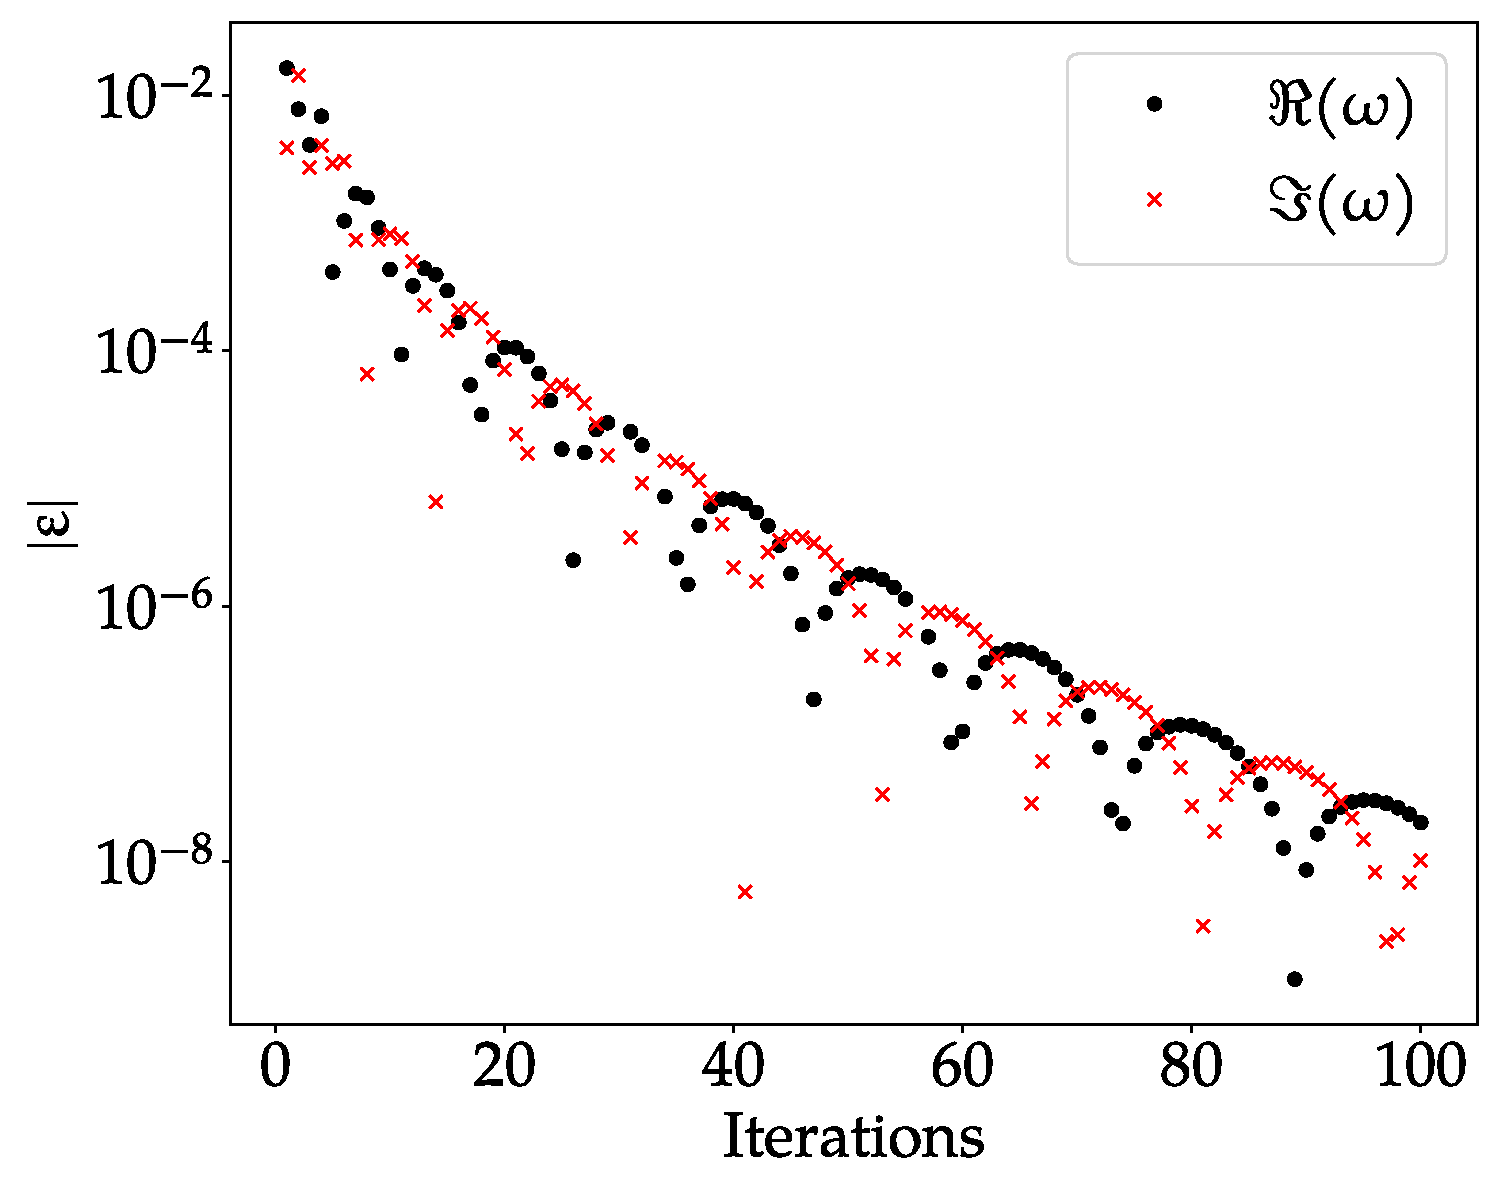
\includegraphics[width=\linewidth]{img/aim_qnm/err.pdf}
  \caption{Error of the fundamental $s=l=0$ Schwarzschild \ac{QNM} vs. the number of \ac{AIM} iterations. Reference values obtained in Ref.~\cite{BertiQNMData}. The y-axis of the plot is in logarithmic scale.}
  \label{fig:package_error}
\end{figure}

\begin{figure}[!ht]
  \centering
  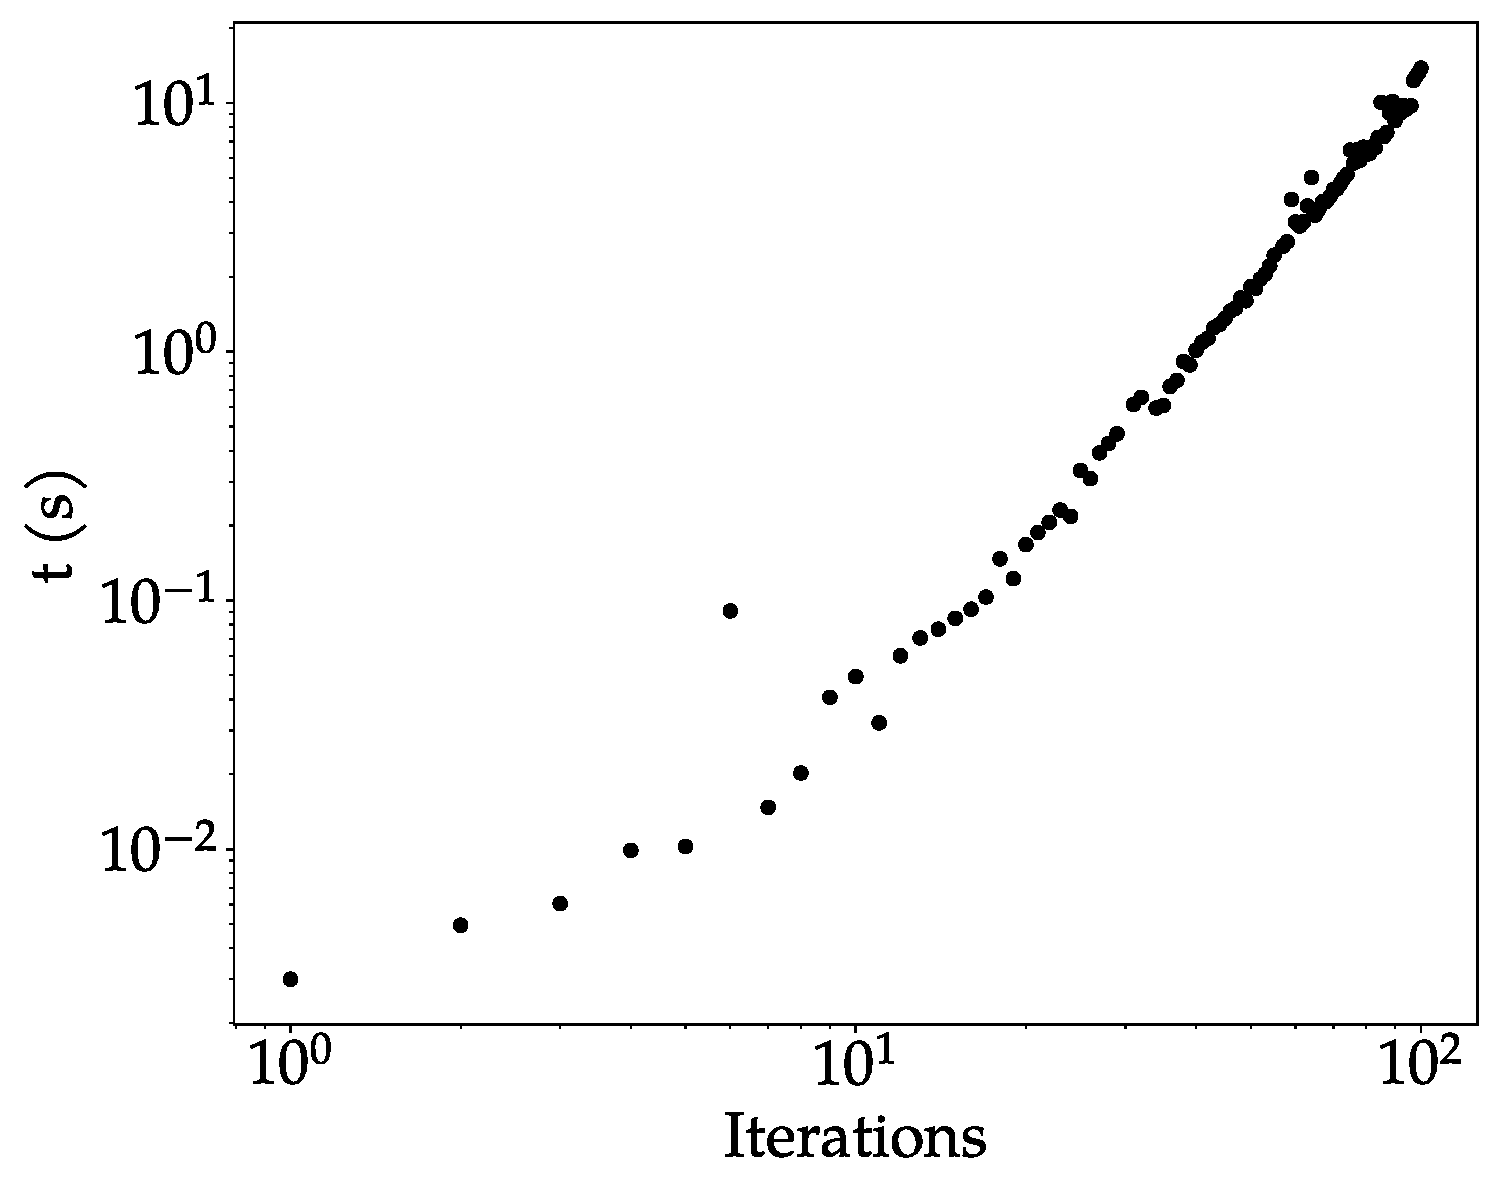
\includegraphics[width=\linewidth]{img/aim_qnm/perf.pdf}
  \caption{Time taken (average of 20 repetitions) vs. the number of \ac{AIM} iterations taken to compute the fundamental Schwarzschild \ac{QNM}. The plot is in a log-log scale.}
  \label{fig:package_perf}
\end{figure}

\section{Results}
\label{ch:qnm_aim:sec:results}
Utilizing \texttt{QuasinormalModes.jl}, we have investigated in Ref.~\cite{Mamani2022} the quasinormal frequencies of asymptotically flat Schwarzschild black holes with spin values of $2$, $1$, $3/2$, $2$, and $5/2$, using both the \ac{AIM} and the pseudo-spectral method. Our goal was to compare and contrast the numerical results obtained with available literature data (when possible). We computed higher overtones quasinormal frequencies for all perturbation fields considered, and found purely imaginary frequencies for the spin $1/2$ and $3/2$ fields, which agree with previous analytical results in the literature. Moreover, we observed that the purely imaginary frequencies for the spin $1/2$ perturbation field are identical to those for the spin $3/2$ perturbation field. In addition, we determined the quasinormal frequencies for the spin $5/2$ perturbation field for the first time, and similarly found purely imaginary frequencies in this case.

This section presents our numerical findings for the quasinormal frequencies of various spin perturbation fields, as shown in Tables \ref{Tab:Spin0}-\ref{Tab:Spin5/2}. Each table includes four columns: the first two display data acquired through the pseudo-spectral method using different numbers of interpolating polynomials, the third column shows results obtained from the \ac{AIM} method using \texttt{QuasinormalModes.jl}, and the fourth and fifth columns are reproductions of literature results, when available. As observed in all data tables, pseudo-spectral method I (computed with $60$ polynomials) and pseudo-spectral method II (computed with $40$ polynomials) produce practically identical results to those generated by \texttt{QuasinormalModes.jl}, with a precision of six decimal places. The numerical methods utilized in this study yield more precise outcomes than those attained previously using the WKB approximation and enable us to compute additional frequencies that have not been reported in previous literature.

We also found purely imaginary frequencies for the spin $1/2$, $3/2$ and $5/2$ fields, reported in Tables \ref{Tab:PurelyImSpin1/2}-\ref{Tab:PurelyImSpin5/2}, respectively. Such frequencies arise when investigating the quasinormal modes in the limit of large $\ell$. Notice that these results are also in agreement with the analytic solutions obtained in the literature but for spin $5/2$ fields, the discrepancy between both methods increases as the imaginary frequency gets more negative. We do not have a concrete explanation for this fact.

\begin{table}[ht]
  \centering
  \resizebox{\linewidth}{!}{%
    \begin{tabular}{l|c|c|c|c|c|c}
      \hline
      $l$ & $n$ & \tlt{Pseudo-spectral}{I (60 Polynomials)} & \tlt{Pseudo-spectral}{II (40 polynomials)} & \tlt{\ac{AIM}}{100 Iterations} & Ref.~\cite{Shu:2005fw} & Ref.~\cite{Konoplya:2004ip} \\ \hline\hline
      0   & $0$ & $\pm 0.110455 -0.104896 i$                & $\pm 0.110455 -0.104896 i$                 & $\pm 0.110455 -0.104896 i$     & $0.1046-0.1152 i$      & $\pm 0.1105-0.1008i$        \\ \hline
      1   & $0$ & $\pm 0.292936 -0.097660 i$                & $\pm 0.292936 -0.097660 i$                 & $\pm 0.292936 -0.097660 i$     & $0.2911-0.0980 i$      & $\pm 0.2929-0.0978i$        \\
          & $1$ & $\pm 0.264449 -0.306257 i$                & $\pm 0.264449 -0.306257 i$                 & $\pm 0.264449 -0.306257 i$     & ---                    & $\pm 0.2645-0.3065i$        \\ \hline
      2   & $0$ & $\pm 0.483644 -0.096759 i$                & $\pm 0.483644 -0.096759 i$                 & $\pm 0.483644 -0.096759 i$     & $0.4832-0.0968 i$      & $\pm 0.4836-0.0968i$        \\
          & $1$ & $\pm 0.463851 -0.295604 i$                & $\pm 0.463851 -0.295604 i$                 & $\pm 0.463851 -0.295604 i$     & $0.4632-0.2958 i$      & $\pm 0.4638-0.2956i$        \\
          & $2$ & $\pm 0.430544 -0.508558 i$                & $\pm 0.430544 -0.508558 i$                 & $\pm 0.430544 -0.508558 i$     & ---                    & $\pm 0.4304-0.5087i$        \\ \hline
      3   & $0$ & $\pm 0.675366 -0.096500 i$                & $\pm 0.675366 -0.096500 i$                 & $\pm 0.675366 -0.096500 i$     & $0.6752-0.0965 i$      & ---                         \\
          & $1$ & $\pm 0.660671 -0.292285 i$                & $\pm 0.660671 -0.292285 i$                 & $\pm 0.660671 -0.292285 i$     & $0.6604-0.2923 i$      & ---                         \\
          & $2$ & $\pm 0.633626 -0.496008 i$                & $\pm 0.633626 -0.496008 i$                 & $\pm 0.633626 -0.496008 i$     & $0.6348-0.4941 i$      & ---                         \\
          & $3$ & $\pm 0.598773 -0.711221 i$                & $\pm 0.598773 -0.711221 i$                 & $\pm 0.598773 -0.711221 i$     & ---                    & ---                         \\ \hline
      4   & $0$ & $\pm 0.867416 -0.096392 i$                & $\pm 0.867416 -0.096392 i$                 & $\pm 0.867416 -0.096392 i$     & $0.8673-0.0964 i$      & ---                         \\
          & $1$ & $\pm 0.855808 -0.290876 i$                & $\pm 0.855808 -0.290876 i$                 & $\pm 0.855808 -0.290876 i$     & $0.8557-0.2909 i$      & ---                         \\
          & $2$ & $\pm 0.833692 -0.490325 i$                & $\pm 0.833692 -0.490325 i$                 & $\pm 0.833692 -0.490325 i$     & $0.8345-0.4895 i$      & ---                         \\
          & $3$ & $\pm 0.803288 -0.697482 i$                & $\pm 0.803288 -0.697482 i$                 & $\pm 0.803288 -0.697482 i$     & $0.8064-0.6926 i$      & ---                         \\
          & $4$ & $\pm 0.767733 -0.914019 i$                & $\pm 0.767733 -0.914019 i$                 & $\pm 0.767733 -0.914019 i$     & ---                    & ---                         \\
      \hline\hline
    \end{tabular}%
  }
  \caption{
    Quasinormal frequencies of the spin $0$ perturbations normalized by the mass $(M\omega)$ compared against the results of Refs.~\cite{Shu:2005fw, Konoplya:2004ip}.
  }
  \label{Tab:Spin0}
\end{table}

\begin{table}[ht]
  \centering
  \resizebox{\linewidth}{!}{%
    \begin{tabular}{l |c|c|c|c|c|c}
      \hline
      $l$ & $n$ & \tlt{Pseudo-spectral}{I (60 Polynomials)} & \tlt{Pseudo-spectral}{II (40 polynomials)} & \tlt{\ac{AIM}}{100 Iterations} & Ref.~\cite{Shu:2005fw} & Ref.~\cite{Konoplya:2004ip} \\ \hline\hline
      1   & $0$ & $\pm 0.248263-0.092488 i$                 & $\pm 0.248263 -0.092488 i$                 & $\pm 0.248263 -0.092488 i$     & $0.2459-0.0931i$       & $\pm 0.2482-0.0926i$        \\
          & $1$ & $\pm 0.214515-0.293668 i$                 & $\pm 0.214515 -0.293667 i$                 & $\pm 0.214515 -0.293668 i$     & ---                    & $\pm 0.2143-0.2941i$        \\ \hline
      2   & $0$ & $\pm 0.457596-0.095004 i$                 & $\pm 0.457595 -0.095004 i$                 & $\pm 0.457596 -0.095004 i$     & $0.4571-0.0951i$       & $\pm 0.4576-0.0950i$        \\
          & $1$ & $\pm 0.436542-0.290710 i$                 & $\pm 0.436542 -0.290710 i$                 & $\pm 0.436542 -0.290710 i$     & $0.4358-0.2910i$       & $\pm 0.4365-0.2907i$        \\
          & $2$ & $\pm 0.401187-0.501587 i$                 & $\pm 0.401187 -0.501587 i$                 & $\pm 0.401187 -0.501587 i$     & ---                    & $\pm 0.4009-0.5017i$        \\ \hline
      3   & $0$ & $\pm 0.656899-0.095616 i$                 & $\pm 0.656899 -0.095616 i$                 & $\pm 0.656899 -0.095616 i$     & $0.6567-0.0956i$       & $\pm 0.6569-0.0956i$        \\
          & $1$ & $\pm 0.641737-0.289728 i$                 & $\pm 0.641737 -0.289728 i$                 & $\pm 0.641737 -0.289728 i$     & $0.6415-0.2898i$       & $\pm 0.6417-0.2897i$        \\
          & $2$ & $\pm 0.613832-0.492066 i$                 & $\pm 0.613832 -0.492066 i$                 & $\pm 0.613832 -0.492066 i$     & $0.6151-0.4901i$       & $\pm 0.6138-0.4921i$        \\
          & $3$ & $\pm 0.577919-0.706331 i$                 & $\pm 0.577919 -0.706331 i$                 & $\pm 0.577919 -0.706330 i$     & ---                    & $\pm 0.5775-0.7065i$        \\ \hline
      4   & $0$ & $\pm 0.853095-0.095860 i$                 & $\pm 0.853095 -0.095860 i$                 & $\pm 0.853095 -0.095810 i$     & $0.8530-0.0959i$       & ---                         \\
          & $1$ & $\pm 0.841267-0.289315 i$                 & $\pm 0.841267 -0.289315 i$                 & $\pm 0.841267 -0.289315 i$     & $0.8411-0.2893i$       & ---                         \\
          & $2$ & $\pm 0.818728-0.487838 i$                 & $\pm 0.818728 -0.487838 i$                 & $\pm 0.818728 -0.487838 i$     & $0.8196-0.4870i$       & ---                         \\
          & $3$ & $\pm 0.787748-0.694242 i$                 & $\pm 0.787748 -0.694242 i$                 & $\pm 0.787748 -0.694242 i$     & $0.7909-0.6892i$       & ---                         \\
          & $4$ & $\pm 0.751549-0.910242 i$                 & $\pm 0.751549 -0.910242 i$                 & $\pm 0.751549 -0.910242 i$     & ---                    & ---                         \\
      \hline\hline
    \end{tabular}%
  }
  \caption{
    Quasinormal frequencies of the spin $1$ perturbations normalized by the mass $(M\omega)$ compared against the results of Refs.~\cite{Shu:2005fw, Konoplya:2004ip}.
  }
  \label{Tab:Spin1}
\end{table}

\begin{table}[ht]
  \centering
  \resizebox{\linewidth}{!}{%
    \begin{tabular}{l |c|c|c|c|c|c}
      \hline
      $l$ & $n$ & \tlt{Pseudo-spectral}{I (60 Polynomials)} & \tlt{Pseudo-spectral}{II (40 polynomials)} & \tlt{\ac{AIM}}{100 Iterations} & Ref.~\cite{Shu:2005fw} & Ref.~\cite{Konoplya:2004ip} \\ \hline\hline
      2   & $0$ & $\pm 0.373672-0.088962i$                  & $\pm 0.373672 -0.088962 i$                 & $\pm 0.373672 -0.088962 i$     & $0.3730-0.0891i$       & $\pm 0.3736-0.0890i$        \\
          & $1$ & $\pm 0.346711-0.273915i$                  & $\pm 0.346711 -0.273915 i$                 & $\pm 0.346711 -0.273915 i$     & $0.3452-0.2746i$       & $\pm 0.3463-0.2735i$        \\
          & $2$ & $\pm 0.301053-0.478277i$                  & $\pm 0.301053 -0.478277 i$                 & $\pm 0.301053 -0.478277 i$     & ---                    & $\pm 0.2985-0.4776i$        \\ \hline
      3   & $0$ & $\pm 0.599443-0.092703i$                  & $\pm 0.599443 -0.092703 i$                 & $\pm 0.599443 -0.092703 i$     & $0.5993-0.0927i$       & $\pm 0.5994-0.0927i$        \\
          & $1$ & $\pm 0.582644-0.281298i$                  & $\pm 0.582644 -0.281298 i$                 & $\pm 0.582644 -0.281298 i$     & $0.5824-0.2814i$       & $\pm 0.5826-0.2813i$        \\
          & $2$ & $\pm 0.551685-0.479093i$                  & $\pm 0.551685 -0.479093 i$                 & $\pm 0.551685 -0.479027 i$     & $0.5532-0.4767i$       & $\pm 0.5516-0.4790i$        \\
          & $3$ & $\pm 0.511962-0.690337i$                  & $\pm 0.511962 -0.690337 i$                 & $\pm 0.511962 -0.690337 i$     & ---                    & $\pm 0.5111-0.6905i$        \\ \hline
      4   & $0$ & $\pm 0.809178-0.094164i$                  & $\pm 0.809178 -0.094164 i$                 & $\pm 0.809178 -0.094164 i$     & $0.8091-0.0942i$       & $\pm 0.8092-0.0942i$        \\
          & $1$ & $\pm 0.796632-0.284334i$                  & $\pm 0.796632 -0.284334 i$                 & $\pm 0.796632 -0.284334 i$     & $0.7965-0.2844i$       & $\pm 0.7966-0.2843i$        \\
          & $2$ & $\pm 0.772710-0.479908i$                  & $\pm 0.772710 -0.479908 i$                 & $\pm 0.772710 -0.479908 i$     & $0.7736-0.4790i$       & $\pm 0.7727-0.4799i$        \\
          & $3$ & $\pm 0.739837-0.683924i$                  & $\pm 0.739837 -0.683924 i$                 & $\pm 0.739837 -0.683924 i$     & $0.7433-0.6783i$       & $\pm 0.7397-0.6839i$        \\
          & $4$ & $\pm 0.701516-0.898239i$                  & $\pm 0.701516 -0.898239 i$                 & $\pm 0.701516 -0.898239 i$     & ---                    & $\pm 0.7006-0.8985i$        \\
      \hline\hline
    \end{tabular}%
  }
  \caption{
    Quasinormal frequencies of spin $2$ perturbations normalized by the mass $(M\omega)$ compared against the results of Refs.~\cite{Shu:2005fw, Konoplya:2004ip}.
  }
  \label{Tab:Spin2}
\end{table}

\begin{table}[ht]
  \centering
  \resizebox{\linewidth}{!}{%
    \begin{tabular}{l |c|c|c|c|c|c}
      \hline
      $l$ & $n$ & \tlt{Pseudo-spectral}{I (60 Polynomials)} & \tlt{Pseudo-spectral}{II (40 polynomials)} & \tlt{\ac{AIM}}{100 Iterations} & Ref.~\cite{Shu:2005fw} & Ref.~\cite{Cho:2003qe} \\ \hline\hline
      0   & $0$ & $\pm 0.182963 -0.096982 i$                & $\pm 0.182963 -0.096982 i$                 & $\pm 0.182963 -0.096824 i$     & ---                    & ---                    \\ \hline
      1   & $0$ & $\pm 0.380037 -0.096405 i$                & $\pm 0.380037 -0.096405 i$                 & $\pm 0.380037 -0.096405 i$     & $0.3786-0.0965 i$      & $0.379 -0.097i$        \\
          & $1$ & $\pm 0.355833 -0.297497 i$                & $\pm 0.355833 -0.297497 i$                 & $\pm 0.355833 -0.297497 i$     & ---                    & ---                    \\ \hline
      2   & $0$ & $\pm 0.574094 -0.096305 i$                & $\pm 0.574094 -0.096305 i$                 & $\pm 0.574094 -0.096305 i$     & $0.5737-0.0963 i$      & $0.574 -0.096i$        \\
          & $1$ & $\pm 0.557015 -0.292715 i$                & $\pm 0.557015 -0.292715 i$                 & $\pm 0.557015 -0.292715 i$     & $0.5562-0.2930 i$      & $0.556 -0.293i$        \\
          & $2$ & $\pm 0.526607 -0.499695 i$                & $\pm 0.526607 -0.499695 i$                 & $\pm 0.526607 -0.499695 i$     & ---                    & ---                    \\ \hline
      3   & $0$ & $\pm 0.767355 -0.096270 i$                & $\pm 0.767355 -0.096270 i$                 & $\pm 0.767355 -0.096270 i$     & $0.7672-0.0963 i$      & $0.767 -0.096i$        \\
          & $1$ & $\pm 0.754300 -0.290968 i$                & $\pm 0.754300 -0.290968 i$                 & $\pm 0.754300 -0.290968 i$     & $0.7540-0.2910 i$      & $0.754 -0.291i$        \\
          & $2$ & $\pm 0.729770 -0.491910 i$                & $\pm 0.729770 -0.491910 i$                 & $\pm 0.729770 -0.491910 i$     & $0.7304-0.4909 i$      & $0.730 -0.491i$        \\
          & $3$ & $\pm 0.696913 -0.702293 i$                & $\pm 0.696913 -0.702293 i$                 & $\pm 0.696913 -0.702293 i$     & ---                    & ---                    \\ \hline
      4   & $0$ & $\pm 0.960293 -0.096254 i$                & $\pm 0.960293 -0.096254 i$                 & $\pm 0.960293 -0.096254 i$     & $0.9602-0.0963 i$      & $0.960 -0.096i$        \\
          & $1$ & $\pm 0.949759 -0.290148 i$                & $\pm 0.949759 -0.290148 i$                 & $\pm 0.949759 -0.290148 i$     & $0.9496-0.2902 i$      & $0.950 -0.290i$        \\
          & $2$ & $\pm 0.929494 -0.488116 i$                & $\pm 0.929494 -0.488116 i$                 & $\pm 0.929494 -0.488116 i$     & $0.9300-0.4876 i$      & $0.930 -0.488i$        \\
          & $3$ & $\pm 0.901129 -0.692520 i$                & $\pm 0.901129 -0.692520 i$                 & $\pm 0.901129 -0.692520 i$     & $0.9036-0.6892 i$      & $0.904 -0.689i$        \\
          & $4$ & $\pm 0.867043 -0.905047 i$                & $\pm 0.867008 -0.905066 i$                 & $\pm 0.867043 -0.905047 i$     & ---                    & ---                    \\
      \hline\hline
    \end{tabular}%
  }
  \caption{
    Quasinormal frequencies of the spin $1/2$ perturbations normalized by the mass $(M\omega)$ compared against the results of Refs.~\cite{Cho:2003qe, Shu:2005fw}.
  }
  \label{Tab:Spin1/2}
\end{table}

\begin{table}[ht]
  \centering
  \resizebox{\linewidth}{!}{%
    \begin{tabular}{l |c|c|c|c|c|c}
      \hline
      $l$ & $n$ & \tlt{Pseudo-spectral}{I (60 Polynomials)} & \tlt{Pseudo-spectral}{II (40 polynomials)} & \tlt{\ac{AIM}}{100 Iterations} & Ref.~\cite{Shu:2005fw} & Ref.~\cite{Chen:2016qii} \\ \hline\hline
      0   & $0$ & $\pm 0.311292 -0.090087 i$                & $\pm 0.311292 -0.090087 i$                 & $\pm 0.311292 -0.090087 i$     & ---                    & $0.3112 -0.0902 i$       \\ \hline
      1   & $0$ & $\pm 0.530048 -0.093751 i$                & $\pm 0.530048 -0.093751 i$                 & $\pm 0.530048 -0.093751 i$     & ---                    & $0.5300 -0.0937 i$       \\
          & $1$ & $\pm 0.511392 -0.285423 i$                & $\pm 0.511392 -0.285423 i$                 & $\pm 0.511392 -0.285423 i$     & ---                    & $0.5113 -0.2854 i$       \\ \hline
      2   & $0$ & $\pm 0.734750 -0.094878 i$                & $\pm 0.734750 -0.094878 i$                 & $\pm 0.734750 -0.094878 i$     & $\pm 0.7346 -0.0949 i$ & $0.7347 -0.0948 i$       \\
          & $1$ & $\pm 0.721047 -0.286906 i$                & $\pm 0.721047 -0.286906 i$                 & $\pm 0.721047 -0.286906 i$     & $\pm 0.7206 -0.2870 i$ & $0.7210 -0.2869 i$       \\
          & $2$ & $\pm 0.695287 -0.485524 i$                & $\pm 0.695287 -0.485524 i$                 & $\pm 0.695287 -0.485524 i$     & ---                    & $0.6952 -0.4855 i$       \\ \hline
      3   & $0$ & $\pm 0.934364 -0.095376 i$                & $\pm 0.934364 -0.095376 i$                 & $\pm 0.934364 -0.095376 i$     & $\pm 0.9343 -0.0954 i$ & $0.9343 -0.0953 i$       \\
          & $1$ & $\pm 0.923502 -0.287560 i$                & $\pm 0.923502 -0.287560 i$                 & $\pm 0.923502 -0.287560 i$     & $\pm 0.9233 -0.2876 i$ & $0.9235 -0.2875 i$       \\
          & $2$ & $\pm 0.902599 -0.483957 i$                & $\pm 0.902599 -0.483957 i$                 & $\pm 0.902599 -0.483957 i$     & $\pm 0.9031 -0.4835 i$ & $0.9025 -0.4839 i$       \\
          & $3$ & $\pm 0.873342 -0.687024 i$                & $\pm 0.873343 -0.687024 i$                 & $\pm 0.873342 -0.687024 i$     & ---                    & $0.8732 -0.6870 i$       \\ \hline
      4   & $0$ & $\pm 1.131530 -0.095640 i$                & $\pm 1.131530 -0.095640 i$                 & $\pm 1.131530 -0.095640 i$     & $\pm 1.1315 -0.0956 i$ & $1.1315 -0.0956 i$       \\
          & $1$ & $\pm 1.122523 -0.287908 i$                & $\pm 1.122523 -0.287908 i$                 & $\pm 1.122523 -0.287908 i$     & $\pm 1.1224 -0.2879 i$ & $1.1225 -0.2879 i$       \\
          & $2$ & $\pm 1.104976 -0.483096 i$                & $\pm 1.104976 -0.483096 i$                 & $\pm 1.104976 -0.483096 i$     & $\pm 1.1053 -0.4828 i$ & $1.1049 -0.4830 i$       \\
          & $3$ & $\pm 1.079852 -0.683000 i$                & $\pm 1.079852 -0.683000 i$                 & $\pm 1.079852 -0.683000 i$     & $\pm 1.0817 -0.6812 i$ & $1.0798 -0.6829 i$       \\
          & $4$ & $\pm 1.048599 -0.889113 i$                & $\pm 1.048596 -0.889115 i$                 & $\pm 1.048599 -0.889113 i$     & ---                    & $1.0484 -0.8890 i$       \\
      \hline\hline
    \end{tabular}%
  }
  \caption{
    Quasinormal frequencies of spin $3/2$ perturbations normalized by the mass $(M\omega)$ compared against the results of Refs.~\cite{Chen:2016qii, Shu:2005fw}.
  }
  \label{Tab:Spin3/2}
\end{table}

\begin{table}[ht]
  \centering
  \resizebox{\linewidth}{!}{%
    \begin{tabular}{l |c|c|c|c}
      \hline
      $l$ & $n$ & \tlt{Pseudo-spectral}{I (60 Polynomials)} & \tlt{Pseudo-spectral}{II (40 polynomials)} & \tlt{\ac{AIM}}{100 Iterations} \\ \hline\hline
      0   & $0$ & $\pm 0.462727-0.092578i$                  & $\pm 0.462727-0.092578i$                   & $0.462727 - 0.092577 i$        \\ \hline
      1   & $0$ & $\pm 0.687103-0.094566i$                  & $\pm 0.687103-0.094566i$                   & $0.687103 - 0.094566 i$        \\
          & $1$ & $\pm 0.670542-0.285767i$                  & $\pm 0.670542-0.285767i$                   & $0.670542 - 0.285767 i$        \\ \hline
      2   & $0$ & $\pm 0.897345-0.095309i$                  & $\pm 0.897345-0.095309i$                   & $0.897345 - 0.095309 i$        \\
          & $1$ & $\pm 0.884980-0.287266i$                  & $\pm 0.884980-0.287266i$                   & $0.884980 - 0.287266 i$        \\
          & $2$ & $\pm 0.861109-0.483113i$                  & $\pm 0.861109-0.483113i$                   & $0.861109 - 0.483113 i$        \\ \hline
      3   & $0$ & $\pm 1.101190-0.095648i$                  & $\pm 1.101190-0.095648i$                   & $1.101190 - 0.095648 i$        \\
          & $1$ & $\pm 1.091300-0.287886i$                  & $\pm 1.091300-0.287886i$                   & $1.091300 - 0.287886 i$        \\
          & $2$ & $\pm 1.071999-0.482895i$                  & $\pm 1.071999-0.482895i$                   & $1.071999 - 0.482895 i$        \\
          & $3$ & $\pm 1.044272-0.682307i$                  & $\pm 1.044272-0.682307i$                   & $1.044272 - 0.682307 i$        \\ \hline
      4   & $0$ & $\pm 1.301587-0.095829i$                  & $\pm 1.301587-0.095829i$                   & $1.301587 - 0.095829 i$        \\
          & $1$ & $\pm 1.293328-0.288184i$                  & $\pm 1.293328-0.288184i$                   & $1.293328 - 0.288184 i$        \\
          & $2$ & $\pm 1.277107-0.482604i$                  & $\pm 1.277107-0.482604i$                   & $1.277107 - 0.482604 i$        \\
          & $3$ & $\pm 1.253526-0.680366i$                  & $\pm 1.253526-0.680366i$                   & $1.253526 - 0.680366 i$        \\
          & $4$ & $\pm 1.223513-0.882554i$                  & $\pm 1.223512-0.882553i$                   & $1.223513 - 0.882554 i$        \\
      \hline\hline
    \end{tabular}%
  }
  \caption{
    Quasinormal frequencies of spin $5/2$ perturbations normalized by the mass $(M\omega)$.
  }
  \label{Tab:Spin5/2}
\end{table}


\begin{table}[t]
  \centering
  \resizebox{\linewidth}{!}{%
    \begin{tabular}{c|c|c}
      \hline
      \tlt{Pseudo-spectral}{I (60 Polynomials)} & \tlt{Pseudo-spectral}{II (40 polynomials)} & \tlt{\ac{AIM}}{100 Iterations} \\ \hline\hline
      $-0.250000i$                              & $-0.250000i$                               & $-0.250000i$                   \\ \hline
      $-0.500000i$                              & $-0.500000i$                               & $-0.500000i$                   \\ \hline
      $-0.750000i$                              & $-0.750000i$                               & $-0.750000i$                   \\ \hline
      $-1.000000i$                              & $-1.000000i$                               & $-1.000031i$                   \\ \hline
      $-1.2499998i$                             & $-1.250000i$                               & $-1.246550i$                   \\
      \hline\hline
    \end{tabular}%
  }
  \caption{
    Purely imaginary frequencies for spin $1/2$ perturbations normalized by the mass $(M\omega)$. The numerical values of such frequencies are exactly the same as for the purely imaginary frequencies arising in the \ac{QNM} of spin $3/2$ perturbations.
  }
  \label{Tab:PurelyImSpin1/2}
\end{table}

\begin{table}[ht]
  \centering
  \resizebox{\linewidth}{!}{%
    \begin{tabular}{c|c|c}
      \hline
      \tlt{Pseudo-spectral}{I (60 Polynomials)} & \tlt{Pseudo-spectral}{II (40 polynomials)} & \tlt{\ac{AIM}}{100 Iterations} \\ \hline\hline
      $-0.250000i$                              & $-0.250000i$                               & $-0.250000i$                   \\ \hline
      $-0.500000i$                              & $-0.500000i$                               & $-0.500000i$                   \\ \hline
      $-0.750000i$                              & $-0.750000i$                               & $-0.750000i$                   \\ \hline
      $-1.000000i$                              & $-1.000000i$                               & $-1.000031i$                   \\ \hline
      $-1.2499998i$                             & $-1.250000i$                               & $-1.246550i$                   \\
      \hline\hline
    \end{tabular}%
  }
  \caption{
    Purely imaginary frequencies for spin $3/2$ perturbations normalized by the mass $(M\omega)$. The numerical values of such frequencies are exactly the same as for the purely imaginary frequencies arising in the \ac{QNM} of spin $1/2$ perturbations.
  }
  \label{Tab:PurelyImSpin3/2}
\end{table}

\begin{table}[ht]
  \centering
  \resizebox{\linewidth}{!}{%
    \begin{tabular}{c|c|c}
      \hline
      \tlt{Pseudo-spectral}{I (60 Polynomials)} & \tlt{Pseudo-spectral}{II (40 polynomials)} & \tlt{\ac{AIM}}{100 Iterations} \\ \hline\hline
      $-0.125000i$                              & $-0.125000i$                               & $-0.125000i$                   \\ \hline
      $-0.375602i$                              & $-0.375602i$                               & $-0.378659i$                   \\ \hline
      $-0.626877i$                              & $-0.626877i$                               & $-0.623931i$                   \\ \hline
      $-0.878946i$                              & $-0.878948i$                               & $-0.907374i$                   \\
      \hline\hline
    \end{tabular}%
  }
  \caption{
    Purely imaginary frequencies of spin $5/2$ perturbations normalized by the mass $(M\omega)$.
  }
  \label{Tab:PurelyImSpin5/2}
\end{table}

\myclearpage
\par

\chapter{Conclusions and perspectives}
\label{ch:conclusion}
In this thesis we have investigated classical phenomena in multiple models of black hole binaries. Specifically, we have analyzed energy extraction, quasinormal modes, and wave scattering around black hole binaries, utilizing numerical, analytical, and semi-analytical techniques. This study has provided the first-ever demonstration of how the phenomena under investigation are altered by the presence of a binary, as compared to their single black hole counterparts.

Regarding the \ac{PP}, we have demonstrated in several comprehensive ways how energy extraction becomes increasingly effective in the presence of charged and rotating binaries. Additionally, we have devised an innovative technique that extends the analysis of energy extraction in a single black hole to arbitrary spacetimes, including numeric ones. We have provided a proof-of-concept example featuring a superimposed Kerr binary, which confirms that the energy extraction efficiency is enhanced by the presence of a secondary object.

Furthermore, a numerical package with broad applicability for computing quasinormal frequencies of black hole spacetimes has been developed. This package employs the recently developed Asymptotic Iteration Method and can easily handle multiple systems, that is, those whose perturbation evolutions can be written as second order ODEs. We have utilized this package to revisit the perturbation problem in the Schwarzschild spacetime, comparing the frequencies computed via the new code with frequencies obtained through traditional pseudospectral methods and values presented in the literature via the WKB approximation or Leaver's continued fraction method. The findings indicate that the results obtained using the \ac{AIM} code are in excellent agreement with available results, thereby enhancing confidence in the method's accuracy and potential to address novel problems. Finally, we have computed new quasinormal frequencies for spin $5/2$ perturbations for the first time, highlighting that these perturbations also possess purely imaginary frequencies.

Lastly, we have elaborated on the creation of a new \texttt{EinsteinToolkit Thorn}, called \texttt{FieldPerturbations}, for the numerical evolution of a scalar field superimposed on a dynamically evolving metric. We have presented preliminary findings concerning the scattering of a massless field over the GW150914 binary collision. Specifically, our results have demonstrated that the field profile displays a damped oscillatory phase following a highly nonlinear scattering, which bears similarities to the behavior observed when perturbing a single black hole. However, distinct differences prohibit direct fitting of a damped sine or cosine to the signal. Given that the run is in its initial stage, and the code remains subject to rigorous testing and development, we must conclude that it is currently impossible to confirm conclusively whether this effect is exclusively attributable to the nonlinear nature of the interaction between the black holes in the binary or to numerical artifacts due to various sources.

We contend that our study has yielded valuable insights and ideas for extending established phenomena to binary systems. We maintain that it is crucial to develop tools and methods capable of extending these analyses to binary black hole spacetime models that lack analytic solutions, given that numerical methods are necessary to capture the full effect of nonlinear interaction in General Relativity. Moreover, we believe that our work represents a crucial step towards this goal and serves to inspire further research in these phenomena.

We propose three potential directions for future research. Firstly, we aim to incorporate our proposed approach for studying the Penrose process in dynamic spacetimes into fully dynamical simulations. We suggest utilizing the \texttt{EinsteinToolkit} infrastructure to compute orbits as a background metric is evolved, or even using tables of a numerically evolved metric as input for the code. Secondly, we contend that it may be possible to separate the perturbation partial differential equations (PDEs) that arise from analytical models of binary spacetimes by employing series approximations to the solutions. This approach would enable the derivation of a system of coupled ordinary differential equations (ODEs) that could, in principle, be solved via the \ac{AIM} or other methods to yield arbitrarily accurate approximations of quasinormal frequencies in these contexts. Finally, we suggest further exploring the numerical simulation of the scalar field on top of the GW150914 binary, searching for potential energy growth via superradiant scattering, analyzing the profile of the field to identify quasinormal frequencies, and investigating other spin perturbations. Additionally, we propose considering the backreaction of the spacetime metric to enhance the realism of the simulations.

\myclearpage
\par

%\appendix

%%%%%%%%%%%%%%%%%%%%%%%%%%%%%
%%% BIBLIOGRAPHY
\bibliographystyle{apsrev4-2}
\bibliography{src/ref_aim.bib,src/ref_books.bib,src/ref_intro.bib,src/ref_owned.bib,src/ref_penrose.bib,src/ref_wave_scattering.bib}

\end{document}
